\documentclass[a4paper,twoside,1pt]{book}


%% === nezbytné balíčky:
\usepackage[T1]{fontenc} % kódování písma
%\usepackage{dsfont} %citace
%\usepackage[nottoc]{tocbibind}      % citace
\usepackage[utf8]{inputenc}     % vstupní znaková sada tohoto dokumentu: UTF-8
\usepackage[nottoc]{tocbibind}
\usepackage{makecell}
\usepackage{nameref}
\usepackage{lmodern}
\usepackage{xargs}
\usepackage[title]{appendix}
\usepackage{import}
\usepackage{pgfplots}
\pgfplotsset{compat=1.18, width=10cm}
\usepackage{subcaption}
\usepackage[font=scriptsize]{caption}
%\usepackage[cp1250]{inputenc}  % vstupní znaková sada tohoto dokumentu: Windows 1250
%\usepackage[latin2]{inputenc}  % vstupní znaková sada tohoto dokumentu: ISO Latin 2

\usepackage[czech]{babel} % česky psaná práce, typografická pravidla. Překládejte pomocí "latex.exe" nebo "pdflatex.exe"
%\usepackage{czech} % česky psaná práce. Překládejte pomocí "pdfCSlatex.exe" ("cslatex.exe" asi bude mít problém s balíkem geometry)

\usepackage[a4paper, hmarginratio=3:2]{geometry} % využití A4 stránky a nastavení okrajů (u vazby bude širší)

\usepackage{pdfpages} % pokud nemáte formulář "Zadání bak./dipl. práce" naskenovaný jako PDF, tak ZAKOMENTUJTE
\usepackage[hidelinks]{hyperref} % v PDF budou klikací odkazy ("hidelinks" je nebude rámovat)

%% === balíčky, které se mohou hodit:
%\usepackage{encxvlna} % postará se o spojky a předložky, které dle českých pravidel nesmí být na konci řádku. Dokumentace: http://texdoc.net/texmf-dist/doc/generic/encxvlna/encxvlna.pdf (chová se správně k "vnitřku" listings?)

\usepackage{graphicx} % balíček pro vkládání rastrových grafických souborů (PNG apod.)
%\usepackage{epsfig} % balíčky pro vkládání grafických souborů typu EPS
\usepackage{float} % rozšířené možnosti umístění obrázků

\usepackage{caption} % pro popisky obrázků, tabulek atd.

\usepackage{tabularx} % rozšířené možnosti tabulek
%\usepackage{tabu} % jiný balík pro rozšířené možnosti tabulek

\usepackage{listings}  % balíček vhodný pro ukázky zdrojového kódu v~textu práce/příloh. Nutno nastavit! http://ftp.cvut.cz/tex-archive/macros/latex/contrib/listings/listings.pdf
\usepackage{amsmath} % balíček pro pokročilou matematickou sazbu
%\usepackage{color} % pro možnost barevného textu
%\usepackage{fancybox} % umožňuje pokročilé rámečkování
\usepackage{fancyhdr} % Tvorba záhlaví a zápatí
\usepackage{adjustbox} %umožnuje upravit velikost tabulek atd.
\usepackage[scientific-notation=true]{siunitx}
\sisetup{exponent-product = \cdot, output-decimal-marker={,}}
%\usepackage{index} % nutno použít v případě tvorby rejstříku balíčkem makeindex
%\usepackage{xcolor} % balíček pro barvy
%\newindex{default}{idx}{ind}{Rejstřík} % zavádí rejstřík v případě použití balíku index


\frenchspacing % za větou bude mezislovní mezera (v anglických textech je mezera za větou delší)
\widowpenalty=1000 % "síla" zákazu vdov (= jeden řádek ze začátku odstavce na konci stránky)
\clubpenalty=1000% "síla" zákazu sirotků (= jeden řádek/slovo z konce odstavce samostatně na začátku stránky)
\brokenpenalty=1000 % "síla" zákazu zlomu stránky za řádkem, který má na konci rozdělené slovo
\raggedbottom         % Nastaví, že místo roztahování textu bude normální hustý text s mezerou
\topmargin=-10mm      % horní okraj trochu menší
\textwidth=150mm      % šířka textu na stránce
\textheight=250mm     % "výška" textu na stránce


\pagenumbering{arabic} % číslování stránek arabskými číslicemi

\fancypagestyle{myheader}{
	\fancyhf{}
	\fancyhead[LE,RO]{\thepage}
	\fancyhead[LO]{\rightmark}
	\fancyhead[RE]{\leftmark}
}

\pagestyle{myheader}      % stránky číslované dole uprostřed

\parindent=2em % odsazení 1. řádku odstavce
\parskip=7pt   % mezera mezi odstavci




%\def\baselinestretch{1.5}\normalsize % nastavím řádkování

\renewcommand{\baselinestretch}{1.1}

\newcommand{\ti}{\textit} % zkrácený příkaz pro kurzívu
\newcommand{\tb}{\textbf} % zkrácený příkaz pro tučné písmo


\captionsetup{font=small, justification=centering} % velikost popisků 


%% --- zde jsou zavedeny některé "konstanty" - některé musíte změnit! --- %%
\newcommand{\cvut}{České vysoké učení technické v~Praze}
\newcommand{\fjfi}{Fakulta jaderná a fyzikálně inženýrská}
\newcommand{\kjr}{Katedra jaderných reaktorů}
\newcommand{\program}{Aplikace přírodních věd} % změňte, pokud máte jiný stud. program
\newcommand{\obor}{Jaderné inženýrství} % změňte, pokud máte jiný obor

\newcommand{\druh}{Výzkumný úkol} % nebo "Diplomová práce"
\newcommand{\woman}{} % pokud jste ŽENA, ZMĚŇTE na: ...{\woman}{a} (je to do Prohlášení)

\newcommand{\logoCVUT}{
\includegraphics{./zadani_logo/symbol_cvut_konturova_verze_cb.pdf}} % logo ČVUT -- podle grafického manuálu ČVUT platného od prosince 2016. Pokud nevyhovuje PDF-verze, tak použijte jinou variantu loga: https://www.cvut.cz/logo-a-graficky-manual -> "Symbol a logo ČVUT v Praze"). Pokud chcete logo úplně vynechat, zadejte místo "\includegraphics{...}" text "\vspace{35mm}"

% přesně podle formuláře "Zadání bak./dipl. práce" VYPLŇTE:
\newcommand{\nazevcz}{Termohydraulický model školního reaktoru VR-1}    % český název práce (přesně podle zadání!)
\newcommand{\nazeven}{Thermohydraulic model of training reactor VR-1}          % anglický název práce (přesně podle zadání!)
\newcommand{\autor}{Bc. Jakub Mátl}   % vyplňte své jméno a příjmení (s akademickým titulem, máte-li jej)
\newcommand{\vedouci}{Ing. Filip Fejt, Ph.D.} % vyplňte jméno a příjmení vedoucího práce, včetně titulů, např.: Doc. Ing. Ivo Malý, Ph.D.
\newcommand{\pracovisteVed}{\kjr, \fjfi, \cvut} % ZMĚŇTE, pokud vedoucí Vaší práce není z KSI
\newcommand{\konzultant}{--} % POKUD MÁTE určeného konzultanta, NAPIŠTE jeho jméno a příjmení
\newcommand{\pracovisteKonz}{--} % POKUD MÁTE konzultanta, NAPIŠTE jeho pracoviště

% podle skutečnosti VYPLŇTE:
\newcommand{\rok}{2023}  % rok odevzdání práce (jen rok odevzdání, nikoli celý akademický rok!)
\newcommand{\kde}{Praze} % studenti z Děčína ZMĚNÍ na: "Děčíně" (doplní se k "prohlášení")

\newcommand{\klicova}{Klíčová slova}   % zde NAPIŠTE česky max. 5 klíčových slov
\newcommand{\keyword}{Key words}       % zde NAPIŠTE anglicky max. 5 klíčových slov (přeložte z češtiny)
\newcommand{\abstrCZ}{Systémové termohydraulické kódy tvoří nedílnou součást analýzy přechodových jevů a nehod na jaderných zařízeních. Prvotní účel těchto kódů byla aplikace na komekční energetické reaktoru, avšak v posledních letech je kladen důraz na validaci těchto kódů pro použití na výzkumných reaktorech. Jedním z problémů systémových kódů je možnost volné nodalizace kontrolních objemů, což může být pro simulaci přirozeného proudění na výzkumných reaktorech zcela zásadní. Cílem práce je aplikace termohydraulického kódu RELAP5/MOD3 k vytvoření termohydraulického modelu školního reaktoru VR-1 a studie vlivu nodalizace na vznik přirozeného proudění.}    % zde NAPIŠTE abstrakt v češtině (cca 7 vět, min. 80 slov)
\newcommand{\abstrEN}{
	System thermohydraulic codes constitute an integral part of the analysis of transients and accidents in nuclear facilities. The initial purpose of these codes was their application to commercial power reactors, but in recent years, emphasis has been placed on validating these codes for use in research reactors. One of the challenges of system-level codes is the free nodalization of control volumes, which can be crucial for simulating natural circulation. The aim of this work is to apply the thermohydraulic code RELAP5/MOD3 to create a thermohydraulic model of the VR-1 research reactor and to study the influence of nodalization on the natural circulation phenomena.} % zde NAPIŠTE abstrakt v angličtině

\newcommand{\prohlaseni}{Prohlašuji, že jsem sůj výzkumný úkol vypracoval\woman{} samostatně a použil\woman{} jsem pouze podklady (literaturu, projekty, SW atd.) uvedené v přiloženém seznamu.} % text prohlášení můžete mírně upravit :-)

\newcommand{\podekovani}{Děkuji Lindě za oběd, měl jsem opravdu hlad.} % NAPIŠTE poděkování, např. svému vedoucímu:
% Děkuji Ing. Eleonoře Krtečkové, Ph.D. za vedení mé bakalářské práce a za podnětné návrhy, které ji obohatily.
% NEBO:
% Děkuji vedoucímu práce doc. Pafnutijovi Snědldítětikaši, Ph.D. za neocenitelné rady a pomoc při tvorbě bakalářské práce.



\begin{document}
%%%%%%%%%%%% TITULNÍ STRANA -- na následujících cca 30 řádků NESAHEJTE!!!  Generuje se AUTOMATICKY %%%%%%%%%%%%
\thispagestyle{empty}

\begin{center}
	{\LARGE
		\cvut\par
		\fjfi
	}
    \vspace{10mm}

    \begin{tabular}{c}
		\tb{\kjr} \\[3pt]   
		\tb{Obor: \obor}\\
    \end{tabular}

   \vspace{10mm} \logoCVUT \vspace{15mm} 

   {\huge \tb{\nazevcz}\par}
   \vspace{5mm}   
   {\huge \tb{\nazeven}\par}
   
   \vspace{15mm}
   {\Large \MakeUppercase{\druh}}

   \vfill
   {\large
    \begin{tabular}{ll}
    Vypracoval: & \autor\\
    Vedoucí práce: & \vedouci\\
    Rok: & \rok
    \end{tabular}
   }
\end{center}

\clearpage{\pagestyle{empty}\cleardoublepage} % prázdná stránka za tou "titulní", bez čísla

%%%%%%%%%%%% ZADÁNÍ PRÁCE %%%%%%%%%%%%
% Zadání (podepsané děkanem!) musíte NASKENOVAT. Ideálně jako 2stránkové PDF (soubor "zadani_cele.pdf"). 
% Před svázáním to v jednom výtisku VYMĚNÍTE ZA ORIGINÁLNÍ ZADÁNÍ (podepsané děkanem fakulty)!
\newpage  % SEM NESAHEJTE!
\thispagestyle{empty} % SEM NESAHEJTE!

%% zde podle toho, jak jste zadání naskenovali, VYBERTE variantu A, B nebo C:
%
% --- varianta A: zadání naskenované jako 2stránkové PDF:
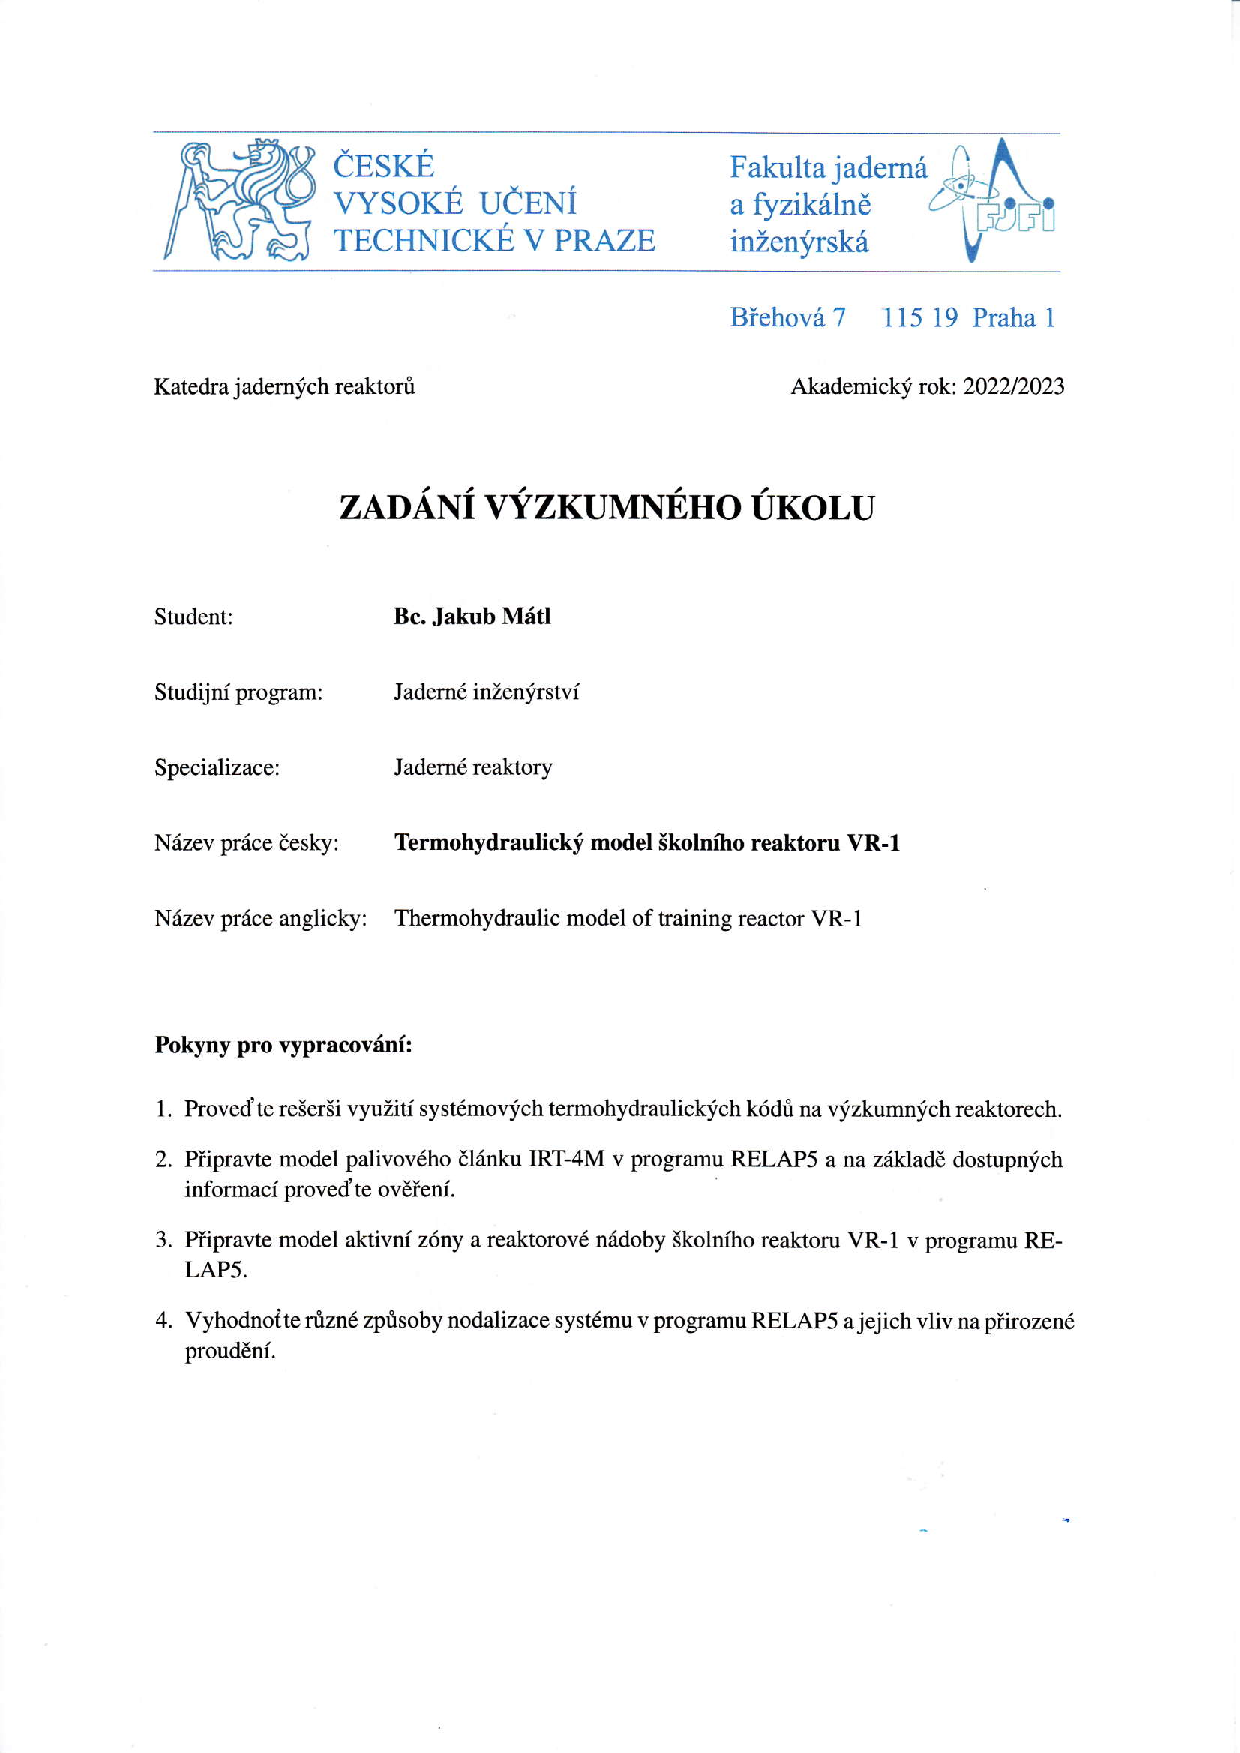
\includepdf[pages={1,2}]{./zadani_logo/zadani_cele.pdf} % NAHRAĎTE správným souborem!
%
%% --- varianta B: zadání naskenované jako jednotlivé stránky:
%\includepdf[pages={1}]{zadani1.pdf} % 1. strana zadání v PDF
%\includepdf[pages={1}]{zadani2.pdf} % 2. strana zadání v PDF
%
%% --- varianta C: zadání naskenované jako 2 samostatné obrázky:
%% 1. strana zadání
%\begin{center}
%     \includegraphics[width=1\textwidth]{zadani1.jpg}
%\end{center}
%% 2. strana zadání
%\newpage  % SEM NESAHEJTE!
%\thispagestyle{empty} % SEM NESAHEJTE!
%\begin{center}
%     \includegraphics[width=1\textwidth]{zadani2.jpg}
%\end{center}


%%%%%%%%%%%% Prohlášení -- SEM NESAHEJTE! Generuje se automaticky z výše nastavených maker \kde{} a \prohlaseni{}. %%%%%%%%%%%%
\newpage % SEM NESAHEJTE!
\thispagestyle{empty}  % SEM NESAHEJTE!

~ % SEM NESAHEJTE!
\vfill % prázdné místo. SEM NESAHEJTE!

\tb{Prohlášení} % SEM NESAHEJTE!

\vspace{1em} % vertikální mezera. SEM NESAHEJTE!
\prohlaseni

\vspace{2em}  % SEM NESAHEJTE!
\hspace{-0.5em}\begin{tabularx}{\textwidth}{X c}  % SEM NESAHEJTE!
V \kde\ dne .................... &........................................ \\	% SEM NESAHEJTE!
	& \autor
\end{tabularx}	% SEM NESAHEJTE!


%%%%%%%%%%%% Poděkování  %%%%%%%%%%%%
\newpage
\thispagestyle{empty}

~
\vfill % prázdné místo


% -- následující kus kódu (do "%%%%%%%%%%%% ABSTRAKT") můžete odstranit, pokud nechcete psát poděkování:
\tb{Poděkování}

\vspace{1em} % vertikální mezera
\podekovani
\begin{flushright}
\autor
\end{flushright}  % <------- tady končí stránka s poděkováním


%%%%%%%%%%%% ABSTRAKT atp. Je generován AUTOMATICKY podle maker nastavených na začátku souboru) %%%%%%%%%%%% 
\newpage   % SEM NESAHEJTE!
\thispagestyle{empty}   % SEM NESAHEJTE!

% příprava:    (na následujících 8 řádků NESAHEJTE!)
\newbox\odstavecbox
\newlength\vyskaodstavce
\newcommand\odstavec[2]{%
    \setbox\odstavecbox=\hbox{%
         \parbox[t]{#1}{#2\vrule width 0pt depth 4pt}}%
    \global\vyskaodstavce=\dp\odstavecbox
    \box\odstavecbox}
\newcommand{\delka}{120mm} % šířka textů ve 2. sloupci tabulky

% použití přípravy:    % dovnitř "tabular" vůbec NESAHEJTE!
\begin{tabular}{ll}
  {\em Název práce:} & ~ \\
  \multicolumn{2}{l}{\odstavec{\textwidth}{\bf \nazevcz}} \\[1em]
  {\em Autor:} & \autor \\[1em]
  {\em Studijní program:} & \program \\
  {\em Obor:} & \obor \\
  {\em Druh práce:} & \druh \\[1em]
  {\em Vedoucí práce:} & \odstavec{\delka}{\vedouci\\ \pracovisteVed} \\
  {\em Konzultant:} & -- %\odstavec{\delka}{\konzultant \\ \pracovisteKonz}  % VYMAŽTE text "-- %" v případě, že jste neměli konzultanta
 \\[1em]  
  \multicolumn{2}{l}{\odstavec{\textwidth}{{\em Abstrakt:} ~ \abstrCZ  }} \\[1em]
  {\em Klíčová slova:} & \odstavec{\delka}{\klicova} \\[2em]

  {\em Title:} & ~\\
  \multicolumn{2}{l}{\odstavec{\textwidth}{\bf \nazeven}}\\[1em]
  {\em Author:} & \autor \\[1em]
  \multicolumn{2}{l}{\odstavec{\textwidth}{{\em Abstract:} ~ \abstrEN  }} \\[1em]
  {\em Key words:} & \odstavec{\delka}{\keyword}
\end{tabular}



%%%%%%%%%%%% Obsah práce ... je generován AUTOMATICKY %%%%%%%%%%%%
\newpage  % SEM NESAHEJTE!
\parskip=0pt
\tableofcontents % SEM NESAHEJTE!
\parskip=7pt
\parskip=0pt
\listoffigures
\parskip=7pt
\parskip=0pt
\listoftables
\parskip=7pt
\newpage % SEM NESAHEJTE!


%--------------------------------------------------------
%|         Zde začíná SAMOTNÁ PRÁCE (text)              |
%--------------------------------------------------------

\chapter*{Úvod} % SEM NESAHEJTE!
\addcontentsline{toc}{chapter}{Úvod} % SEM NESAHEJTE!

\input{./01_uvod/uvod.tex}
\chapter{Termohydraulické systémové kódy}

\section{Úvod}
%Zajištění bezpečnosti jaderného zařízení, resp. jaderného reaktoru je primárním cílem od výstavby, provozu až po vyřazení z provozu. Jedním z mnoha prostředků sloužících k zajištění bezpečnosti jaderného zařízení jsou bezpečnostní analýzy, které se dělí na deterministické analýzy (neutronické, termohydraulické, termomechanické, strukturální a radiační) a pravděpodobnostní hodnocení zařízení. K deterministickému hodnocení bezpečnosti jsou třeba kvalifikované nástroje, čímž jsou mimo jiné také systémové termohydraulické kódy (SYS-TH - system thermal hydraulics). \cite{bestion2017structure, SUJB_zprava}
Systémové termohydraulické kódy (SYS-TH) tvoří nedílnou součást bezpečnostních analýz. Simulace poskytují informace o příslušných parametrech systému, jako jsou tlak, teplota chladiva nebo průtok v kontrolních objemech a teploty materiálů v modelovaných strukturách, to vše v závislosti na čase. SYS TH kódy jsou obvykle založeny na řešení pěti nebo šesti nehomogenních rovnic zachování hmotnosti, energie a hybnosti, obvykle s použitím implicitních nebo poloimplicitních schémat. Prostřednictvím těchto kódů lze simulovat provoz a chování reaktoru, včetně průběhu havárií, a posoudit tak úroveň bezpečnosti jaderné elektrárny \cite{bestion2017structure, petruzzi2008thermal}.

\section{Oblasti aplikace}
Systémové kódy jsou považovány za multifyzikální výpočetní programy schopné simulovat jak základní fyzikální jevy (např. var na stěně trubky), tak i celistvé chování systémů (např. primárního okruhu jaderné elektrárny). Díky tomu je možné pomocí těchto kódů počítat i složité přechodové jevy, které mohou představovat například základní projektové události a nehody na jaderném zařízení. Kromě termohydraulického popisu přenosu hmoty, hybnosti a energie je možné aplikovat SYS-TH kódy na:
\begin{itemize}
	\item popis transportu plynů ($ \text{N}_{2},\,\text{H}_{2},$ vzduch, produkty štěpení...),
	\item transport bórů a těkavých plynů,
	\item kondukce skrze materiály s konvekcí do tekutin,
	\item zjednodušený neutronický popis,
	\item chemický popis reakcí zinku s vodou,
	\item popis chování paliva,
	\item popis chování součástek jaderných elektráren jako rotorů či ventilů,
	\item popis řídících systémů (Instrumentation \& Control).
	
\end{itemize}

V oblasti jaderného inženýrství se používá řada nejmodernějších termohydraulických kódů. Mezi nejpoužívanější kódy patří RELAP5, TRACE, APROS, POLKA-T, CATHARE, ATHLET a RETRAN. Tyto kódy využívají přístup založený na kontrolních objemech s velkou nodalizací a aplikují nejmodernější termohydraulické modely k popisu fyzikálního chování systému \cite{petruzzi2008thermal}.
\section{Hodnocení systémových kódů}
Nedílnou součástí vývoje numerických SYS-TH kódů a jejich interního hodnocení je verifikace a validace. Verifikace i validace se týká procesu zvyšování spolehlivosti kódu a snižování rizika nesprávné aplikace. Interní hodnocení kódu obvykle provádí vývojář kódu.


Verifikace kódu se týká zkoumání zdrojového kódu ve vztahu k jeho popisu v dokumentaci. Tento proces zahrnuje postupy související se zajištěním kvality softwaru a úsilí o odhalení a opravu chyb v modelech a numerických algoritmech využívaných k řešení parciálních diferenciálních rovnic \cite{petruzzi2008thermal}.

Validace kódu zahrnuje vyhodnocení přesnosti předpovídaných hodnot porovnáním s příslušnými experimentálními údaji. Validace kódu se v podstatě zaměřuje na kvantitativní posouzení přesnosti kódu porovnáním s kvalitními validačními experimenty a benchmarkovými úlohami. Tyto experimenty jsou důkladně zdokumentovány a charakterizovány, včetně pečlivých odhadů statistické chyby měření. Díky validačnímu procesu jsou výsledky kódu konzistentní a prokazují, že celý systém může přinášet smysluplné a očekávané výsledky \cite{petruzzi2008thermal}. Proces interního hodnocení kódu je ilustrován na obrázku \ref{fig:v_v_sean_prezentace}.
\begin{figure}[H]
	\centering
	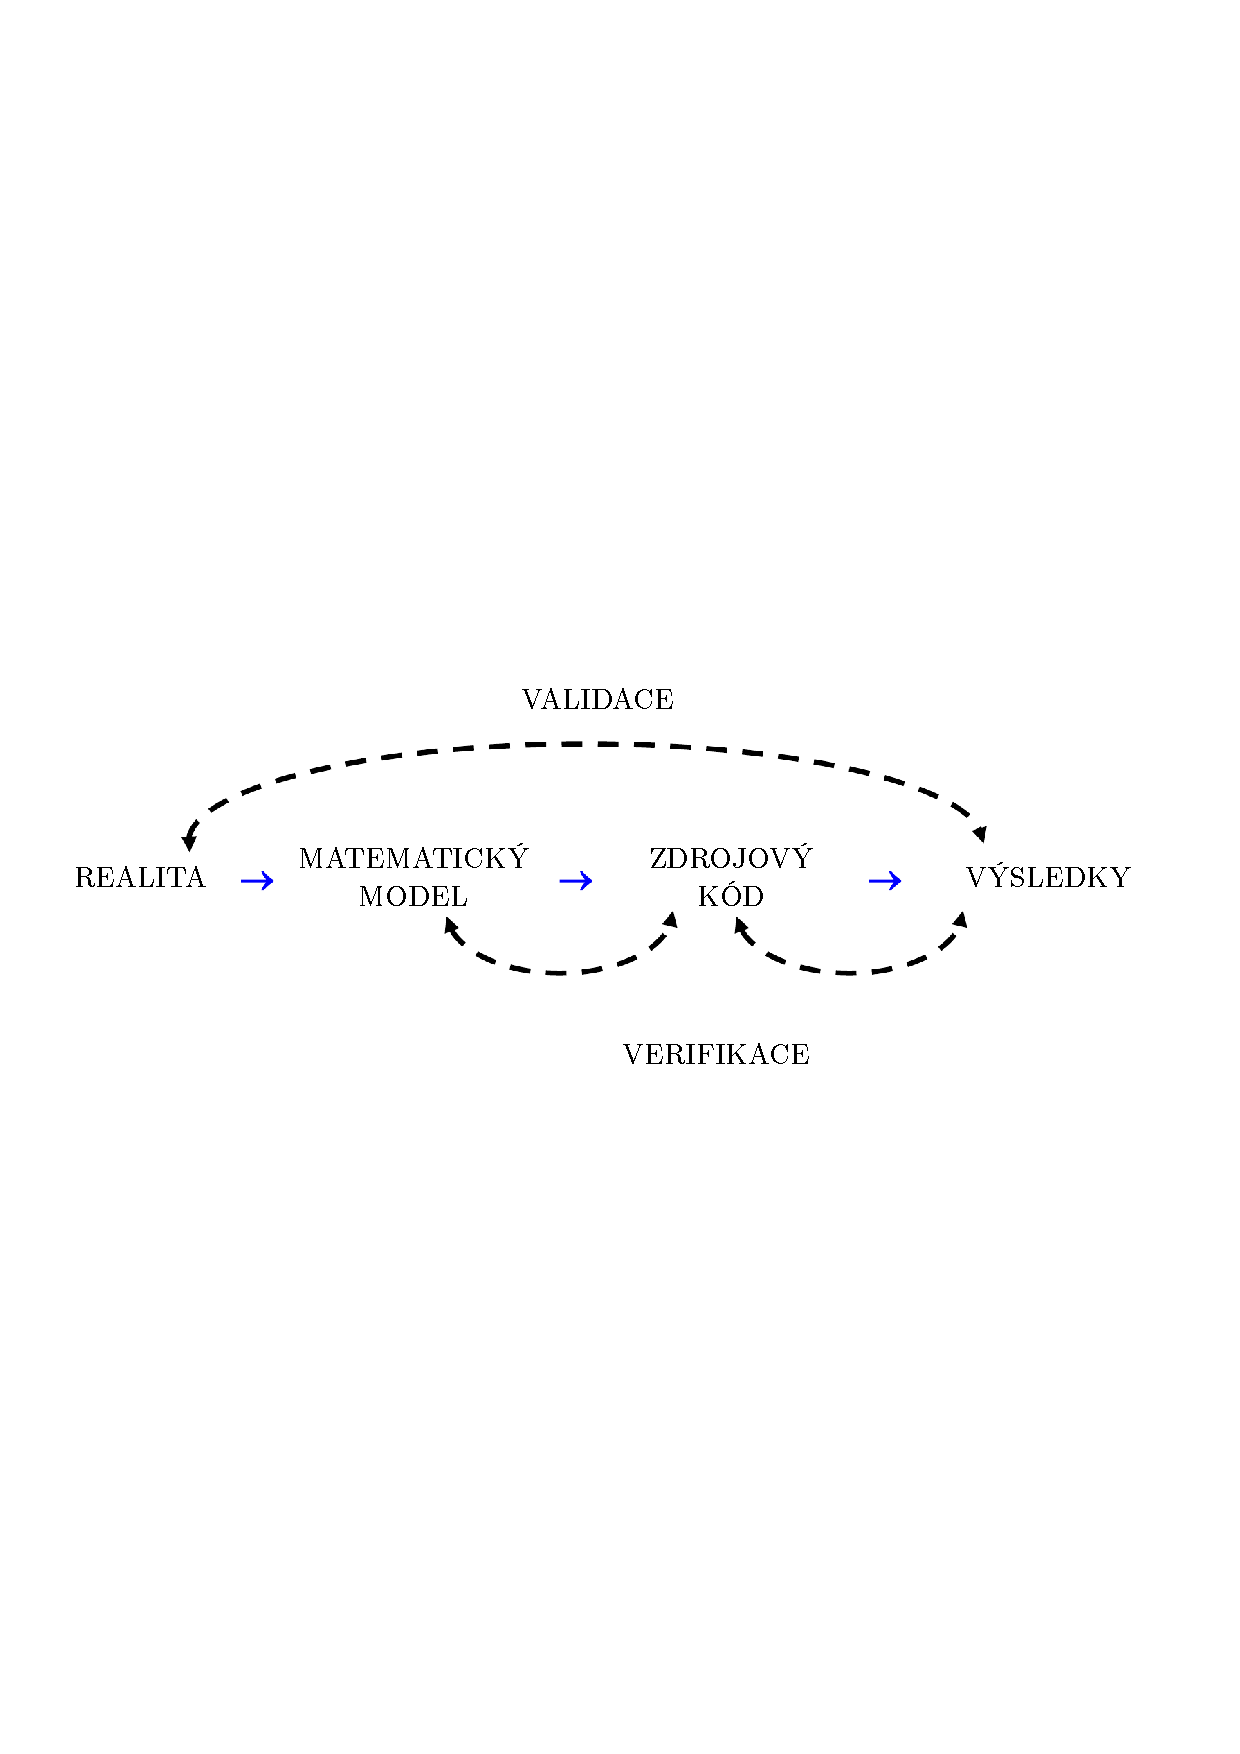
\includegraphics[width=0.8\textwidth, trim={0cm 10cm 0cm 10cm}, clip]{./02_teorie/obrazky/v_v_sean_lectures.pdf}
	\caption{Proces interního hodnocení kódu.}
	\label{fig:v_v_sean_prezentace}
\end{figure}

Interní hodnocení kódu ovšem nemusí vždy identifikovat nepřesnosti kódu při popisu různých fyzikálních jevů. Součástí neustálého vývoje je také externí hodnocení nezávislými institucemi a uživateli. Nezávislé posouzení kódu je proces, kdy třetí strana kvantifikuje přesnost kódu na základě experimentů provedených v integrálním zkušebním zařízení (ITF). Externí posouzení kódu obvykle vyžaduje kvalifikaci uživatele a vhodně zvolenou nodalizaci kontrolních objemů \cite{petruzzi2008thermal}. 

%
%  která je prováděna například srovnáním výsledků s škálovanými experimenty či s daty přímo z jaderné elektrárny. Přestože termohydraulické kódy byly (a stále jsou) za poslední tři dekády neustále vyvíjeny, získávané výsledky jsou stále zatíženy chybami, které mohou být způsobeny nepřesnostmi numerického řešení, nevhodně zvolenými vztahy, nedostatkem znalostí okrajových a počátečních podmínek či efekty nodalizace. 
%\cite{petruzzi2008thermal}


%V závislosti na typu popisované součástky jsou systémové kódy schopné modelovat 0-D, 1-D či 2-D a 3-D geometrie. 0-D model se ve většině případů používá při popisu součástek, ve kterých dochází k velmi nízkým rychlostem proudění, např. kompenzátor objemu. 1-D popis se aplikuje především na součástky s jedním směrem proudění (např. trubky). 2-D a 3-D slouží k analýze součástek náročných na popis (např. AZ reaktoru) \cite{bestion2017structure}. 


\section{Limitace systémových kódů}
Většina užívaných systémových kódů má možnost volné nodalizace jednotlivých termohydraulických komponent. K popisu komplexních problémů se využívají definované komponenty, které jsou děleny na jednotlivé kontrolní objemy. Toto dělení je čistě na uživateli, a neexistuje tedy správný postup, jakou nodalizaci komponent a strukturu studované problematiky použít \cite{petruzzi2008thermal}.

Problematická se může jevit především výše zmíněná nodalizace. Využitím jemnějšího rozdělení je sice možné docílit podrobnějšího popisu, ovšem při nevhodně zvolené nodalizaci, např. přílíš malých kontrolních objemech může docházet k nestabilnímu výpočtu a fyzikálně neodpovídajícím výsledkům. Důvody proč příliš jemná nodalizace může být problematická jsou dva \cite{petruzzi2008thermal}:
\begin{itemize}
	\item velká část empirických vztahů zahrnutých do programu je získána z výpočtu s pevně danou nodalizací, což již z principu vede k rozdílným podmínkám,
	\item numerické simulace využívané v systémových kódech využívají uměle vloženou viskozitu za účelem získání stabilních výsledků.
\end{itemize}

%Dalším aspektem při popisu komplexního problému je propojení jednotlivých součástek, které může mít značný vliv na výsledné proudění. Systémové kódy ve většině případů nabízejí model vytvořit z jednoduchých komponent, a proto je nutné při tvorbě modelu použít "inženýrský odhad" a využít zkušenosti uživatele \cite{petruzzi2008thermal}. 

Důležitá je také široká škála parametrů používaných k popisu fyzikálních jevů. Ne zřídka má uživatel možnost volit mezi dvěma a více vstupními parametry, které k popisu dané problematiky slouží. Příkladem může být například volba mezi různými modely škrcení, nucené proudění podchlazené či nasycené kapaliny nebo nastavení ztrátového součinitele v případě trubek či pístů. Při tvorbě komplexního modelu není neobvyklé, že počet vstupních parametrů se pohybuje v řádu tisíců. Z tohoto důvodu je pravděpodobnost lidské chyby vysoce pravděpodobná a je třeba dbát nesmírné pozornosti při konstrukci modelu. Je vhodné také zmínit často diskutované téma volby časového kroku na řešení a způsobu zadávání okrajových podmínek \cite{petruzzi2008thermal}.

\section{Aplikace na výzkumné reaktory}
Výpočetní kód RELAP5 byl vyvinut jakožto systémový "best-estimate" kód pro popis PIE (postulovaných iniciačních událostí) na konvenčních lehkovodních reaktorech. Množství experimentálně určených vztahů a korelací použitých při vývoji kódu RELAP5 bylo odvozeno a stanoveno právě pro využití na energetických reaktorech, avšak cílem mnohých studií (např. \cite{REIS2012300, CHATZIDAKIS2013341, AZZOUNE2010823}) je aplikace i na výzkumné reaktory \cite{HEDAYAT2017953}. Přestože jsou SYS-TH hojně používány pro bezpečnostní analýzy výzkumných reaktorů, mnohé práce (\cite{international1992iaea, OMAR2010572, CHATZIDAKIS_ASSESMENT_RSG}) upozorňují na nedostatečnou validaci a verifikaci modelů u přechodových jevů a postulovaných iniciačních událostí.  Pro většinu výzkumných reaktorů je kromě jiného také důležitý správný popis odvodu tepla dlouhodobou přirozenou konvekcí. Proto je často kladen důraz na zkušenost uživatele a na \uv{inženýrský odhad} při konstrukci a volbě vstupních parametrů \cite{bestion2017structure}. Z těchto důvodů jsou tvořeny benchmarkové úlohy prováděné právě na výzkumných reaktorech viz např. \cite{international2022iaea_benchmark_database}.

Problém modelování přirozeného proudění se může stát ještě složitějším kvůli přítomnosti dodatečných obtoků a velké redistribuci toku během přechodových jevů. Je na uživateli kódu, aby určil, jak konstruovat takto komplexní proudění v rámci jednorozměrného kódu. K dostatečnému popisu můžou být použity kontrolní objemy, jednoduché a vícenásobné spojovací jednotky či další termohydraulické komponenty. Volba nodalizace a způsobu konstrukce reaktoru by v ideálním případě založena na výsledcích detailních citlivostních analýz. Nicméně v mnoha případech je uživatel nucen učinit ad hoc rozhodnutí kvůli nedostatku času nebo vhodných experimentálních dat \cite{petruzzi2008thermal}.





\chapter{Benchmarková úloha}


Pro model školního reaktoru VR-1 je důležitý přestup tepla v malých rychlostech a nebo při přirozeném proudění. Cílem tvorby benchmarkové úlohy bylo získat praxi v simulaci přestupu tepla při tlacích blízkých atmosférickému tlaku a tyto zkušenosti dále využít při tvorbě modelu VR-1. Proto byl vytvořen jednoduchý model experimentální smyčky vycházející z \cite{zeitoun1994subcooled}. Z \cite{KONCAR2003255} vyplývá, že program RELAP5 je již schopný sdílení tepla při nízkých tlacích simulovat. Proto je možné vytvořený model srovnat s experimentem a ověřit správnost modelu.
\section{Popis experimentu}  
Experimenty popisované v \cite{zeitoun1994subcooled} se týkaly podchlazeného varu a kondenzace ve vertikálním kanálu. Postup zahrnoval cirkulaci vody kanálem, která byla před vstupem do průtočného kanálu v podchlazeném stavu s teplotou pod bodem varu. Poté byla kapalina ohřívána konstantní rychlostí a tepelný tok byl měřen pomocí termočlánku. Jedním z hlavních sledovaných parametrů byl dutinový koeficient, resp. jeho průběh skrze testovací sekci.

Při experimentu byl použit kruhový kanál z nerezové oceli s hladkým vnitřním povrchem a průměrem 5 mm. Kanál byl navržen tak, aby jím mohla protékat voda, a byl vybaven topným systémem, který umožňoval řízený ohřev kapaliny. Voda použitá v experimentu byla zpočátku skladována v nádrži a čerpána kruhovým kanálem s řízeným průtokem. Průtok vody se měřil pomocí průtokoměru umístěného před kanálem. Na vstupu a výstupu kanálu byl rovněž umístěn termočlánek, který měřil teplotu vody před průchodem kanálem a po něm. Kanál byl ohříván pomocí ohříváku, který umožňoval nastavení příkonu. Tepelný tok byl měřen pomocí termočlánku umístěného na vnějším povrchu kanálu. Pro studium varu a kondenzace vody v testovací sekci byl experiment proveden při různých tepelných tocích a průtocích. Tepelný tok se postupně zvyšoval nastavením příkonu topného systému a zaznamenávala se odpovídající teplota vody. Experimentální sestava je ilustrována na Obr. \ref{fig:zeitoun_geometrie} a \ref{fig:zeitoun_circuit}. 


%\begin{figure}
%	\centering
%	\begin{minipage}{.5\textwidth}
%		\centering
%		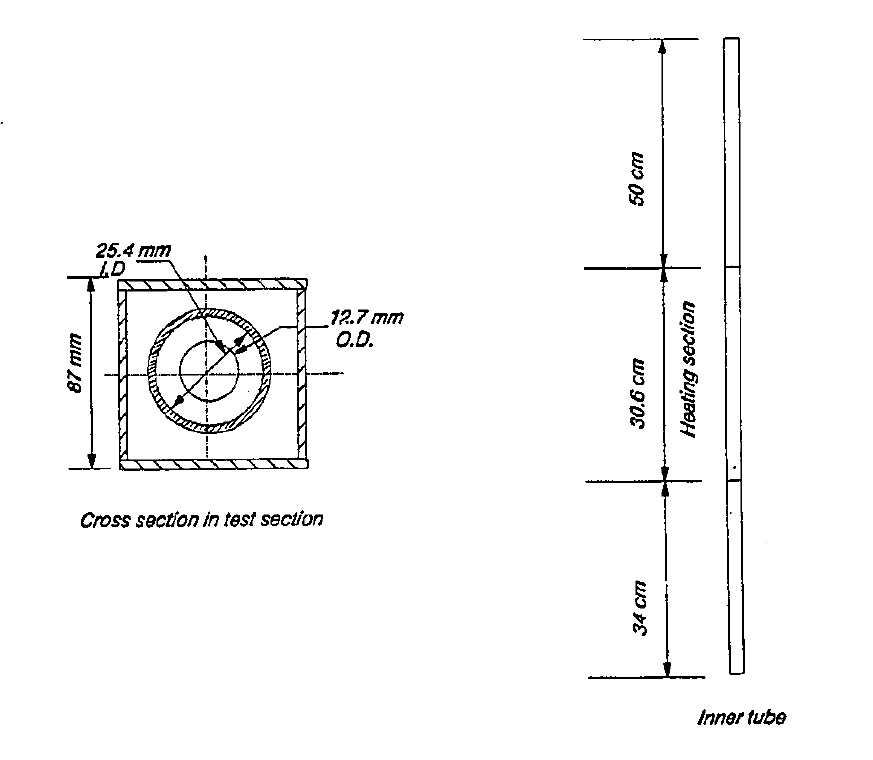
\includegraphics[width=.4\linewidth]{./03_benchmark/obrazky/zeitoun_geometrie.png}
%		\caption{Geometrie testovací trubice \cite{zeitoun1994subcooled}.}
%		\label{fig:zeitoun_geometrie}
%	\end{minipage}%
%	\begin{minipage}{.5\textwidth}
%		\centering
%		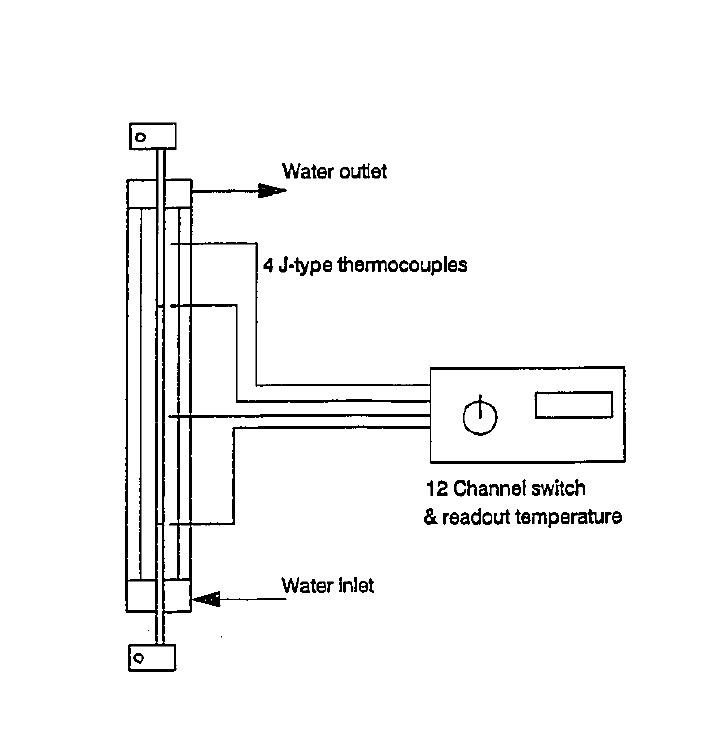
\includegraphics[width=.4\linewidth]{./03_benchmark/obrazky/zeitoun_circuit.png}
%		\caption{Testovací smyčka \cite{zeitoun1994subcooled}.}
%		\label{fig:zeitoun_circuit}
%	\end{minipage}
%\end{figure}
\begin{figure}
	\centering
	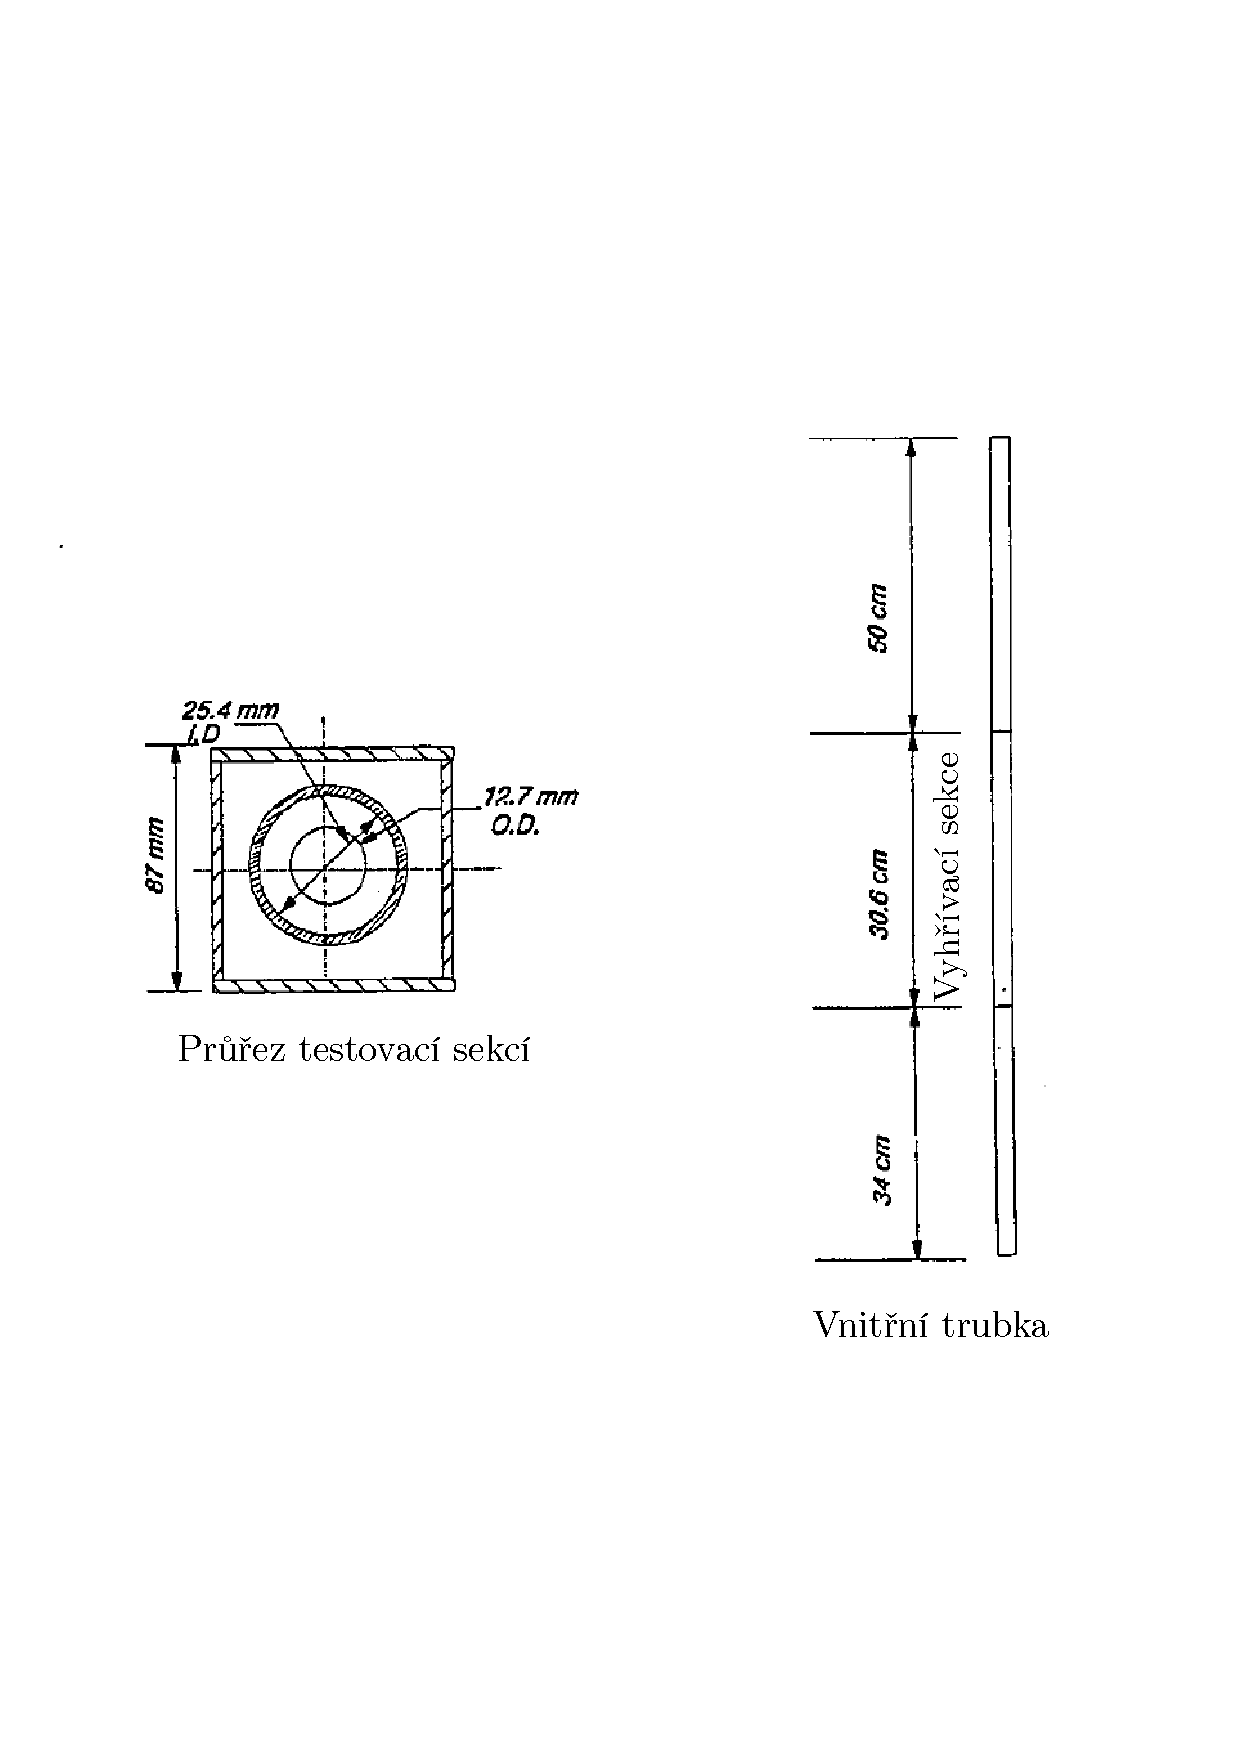
\includegraphics[width=0.8\textwidth, trim={0cm 8cm 0cm 8cm}, clip]{./03_benchmark/obrazky/zeitoun_geometrie_translated.pdf}
	\caption{Geometrie testovací trubice \cite{zeitoun1994subcooled}.}
	\label{fig:zeitoun_geometrie}
\end{figure}

\begin{figure}
	\centering
	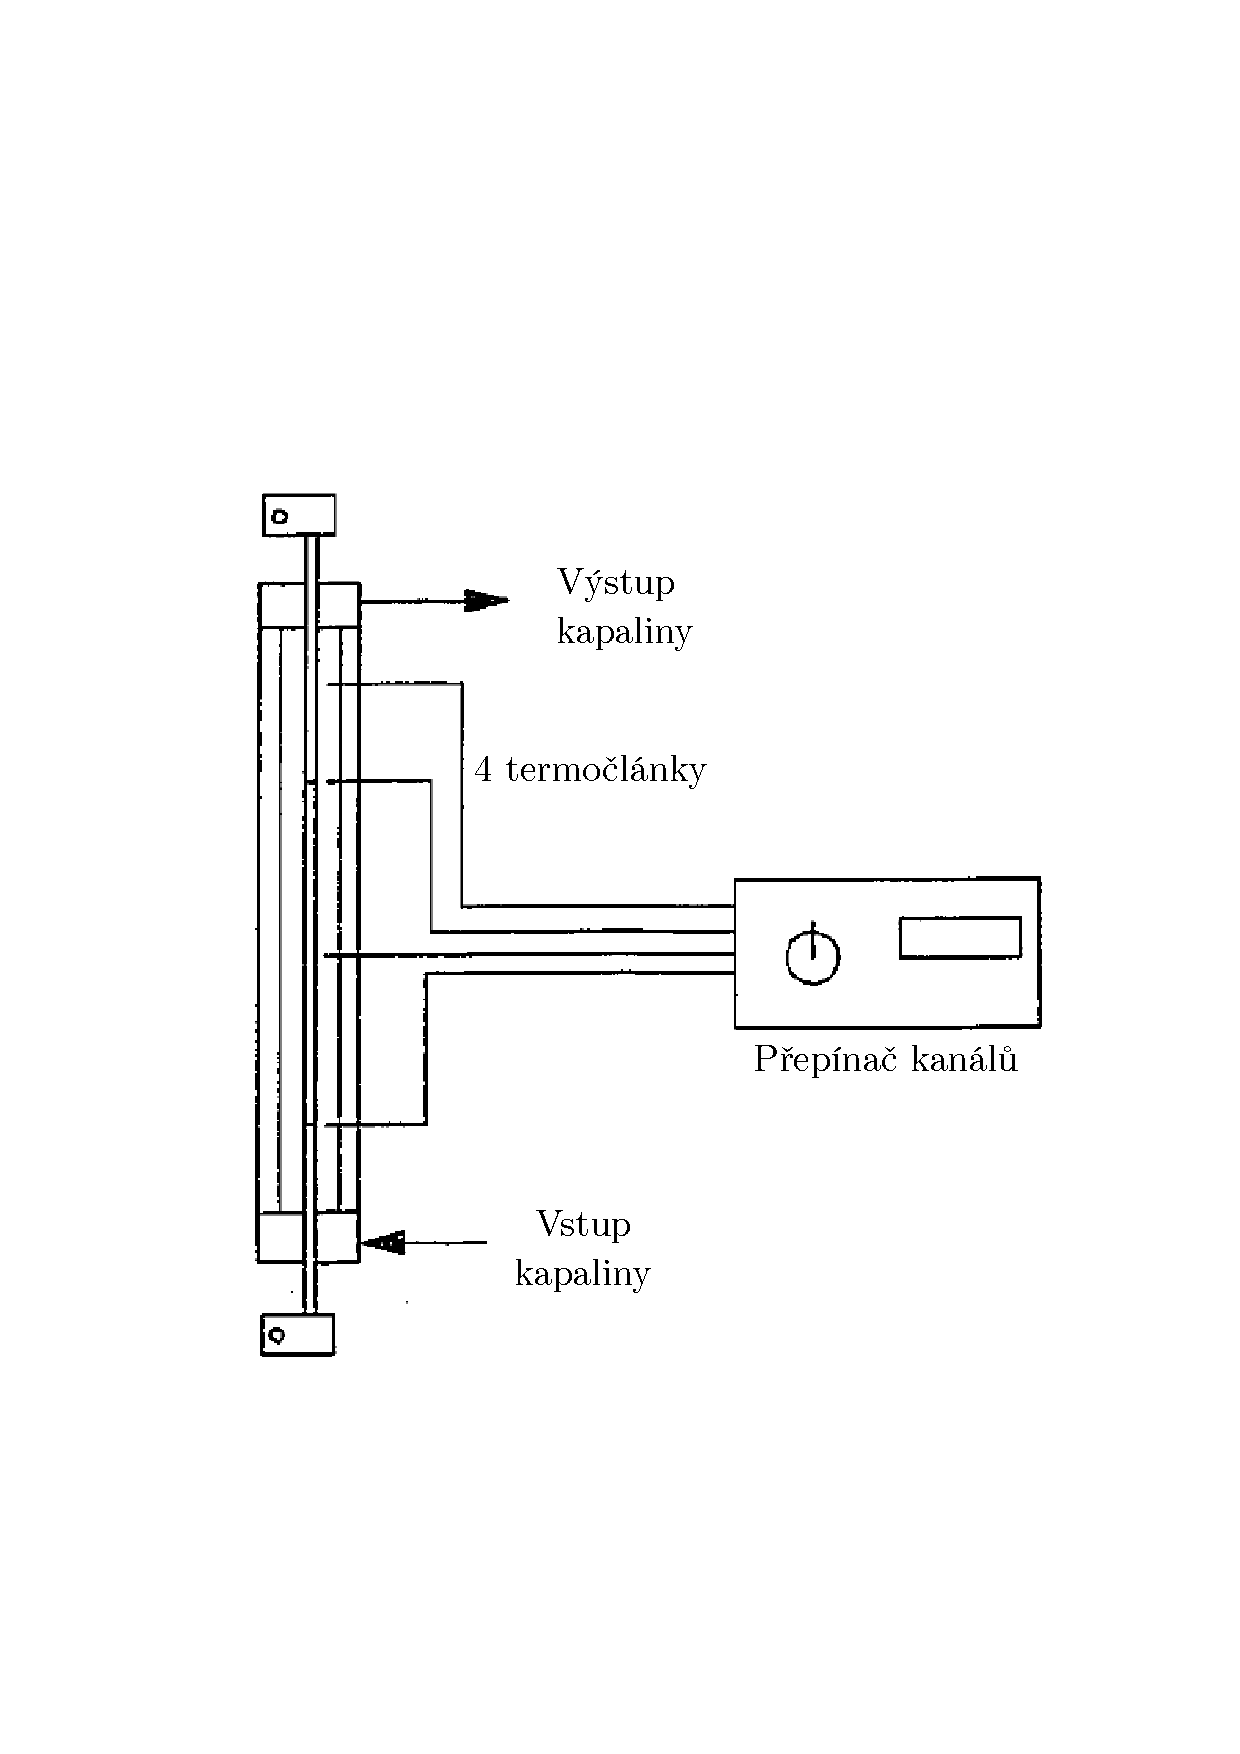
\includegraphics[width=0.8\textwidth, trim={0cm 5cm 0cm 8cm }, clip]{./03_benchmark/obrazky/zeitoun_circuit_translated.pdf}
	\caption{{Testovací smyčka \cite{zeitoun1994subcooled}.}}
	\label{fig:zeitoun_circuit}
\end{figure}


Během experimentu byly rovněž použity vysokorychlostní kamery, které pořizovaly snímky procesů varu a kondenzace uvnitř kanálu. To umožnilo podrobnější analýzu příslušných mechanismů přenosu tepla, jako například průběh dutinového koeficientu.
\section{Základní hydraulické komponenty v kódu RELAP5}
Vzhledem k tomu, že systémový kód RELAP5 využívá konstitutivní rovnice vycházející z teorie podobnosti, tak je uživatel nucen daný problém popsat pomocí přednastavených komponent. Dalším důvodem, proč je těchto komponent využíváno je usnadněná konvergence, která ovšem nemusí být pro komplexní modely nikdy zcela zajištěna. Program RELAP5 obsahuje celkem 17 typů komponent, avšak v této práci bude využito následujících 5 (Obr. \ref{fig:components_relap}). 
\begin{enumerate}
	\item Komponenta 1 - Kontrolní objemy představují konečnou oblast kapalinového systému, například potrubí nebo nádrž, v níž se předpokládají rovnoměrné vlastnosti kapaliny. Pro popis těchto vlastností jsou aplikovány jednorozměrné rovnice proudění.
	\item Komponenta 2 - Trubky slouží k přepravě kapalin z jednoho místa v systému na druhé. V kódu RELAP5 jsou potrubí reprezentována jako řada řídicích. Průtok kapaliny, tlakové ztráty a přenos tepla v potrubí se počítají pomocí jednorozměrných rovnic proudění.
	\item Komponenta 3 - Spojovací jednotky slouží k propojení dvou libovolných komponent. Jsou tvořeny kontrolním objemem, přičemž jsou zde aplikovány rovnice hmotnostní a energetické bilance.
	\item Komponenta 4 - Spojovací jednotky umožňují propojit i více komponent, které mají např. omezené množství výstupních cest. Plní funkci spojovací jednotky pro více komponent.
	\item Komponenta 5 - Objem/zdroj kapaliny sloužící ke stanovení okrajových podmínek (TDV).
	
\end{enumerate}  


Dále jsou v této práci využity tepelné jednotky (Heat structures) představující zdroj tepla. Přenos je popisován jednorozměrnými rovnicemi pro kondukci, konvekci a radiaci pro válcový, deskový či kulový zdroj. V této práci byly využity zdroje pouze válcové popsané výškou a vnějším a vnitřním průměrem \cite{relap_manual}.
\begin{figure}[H]
	\centering
	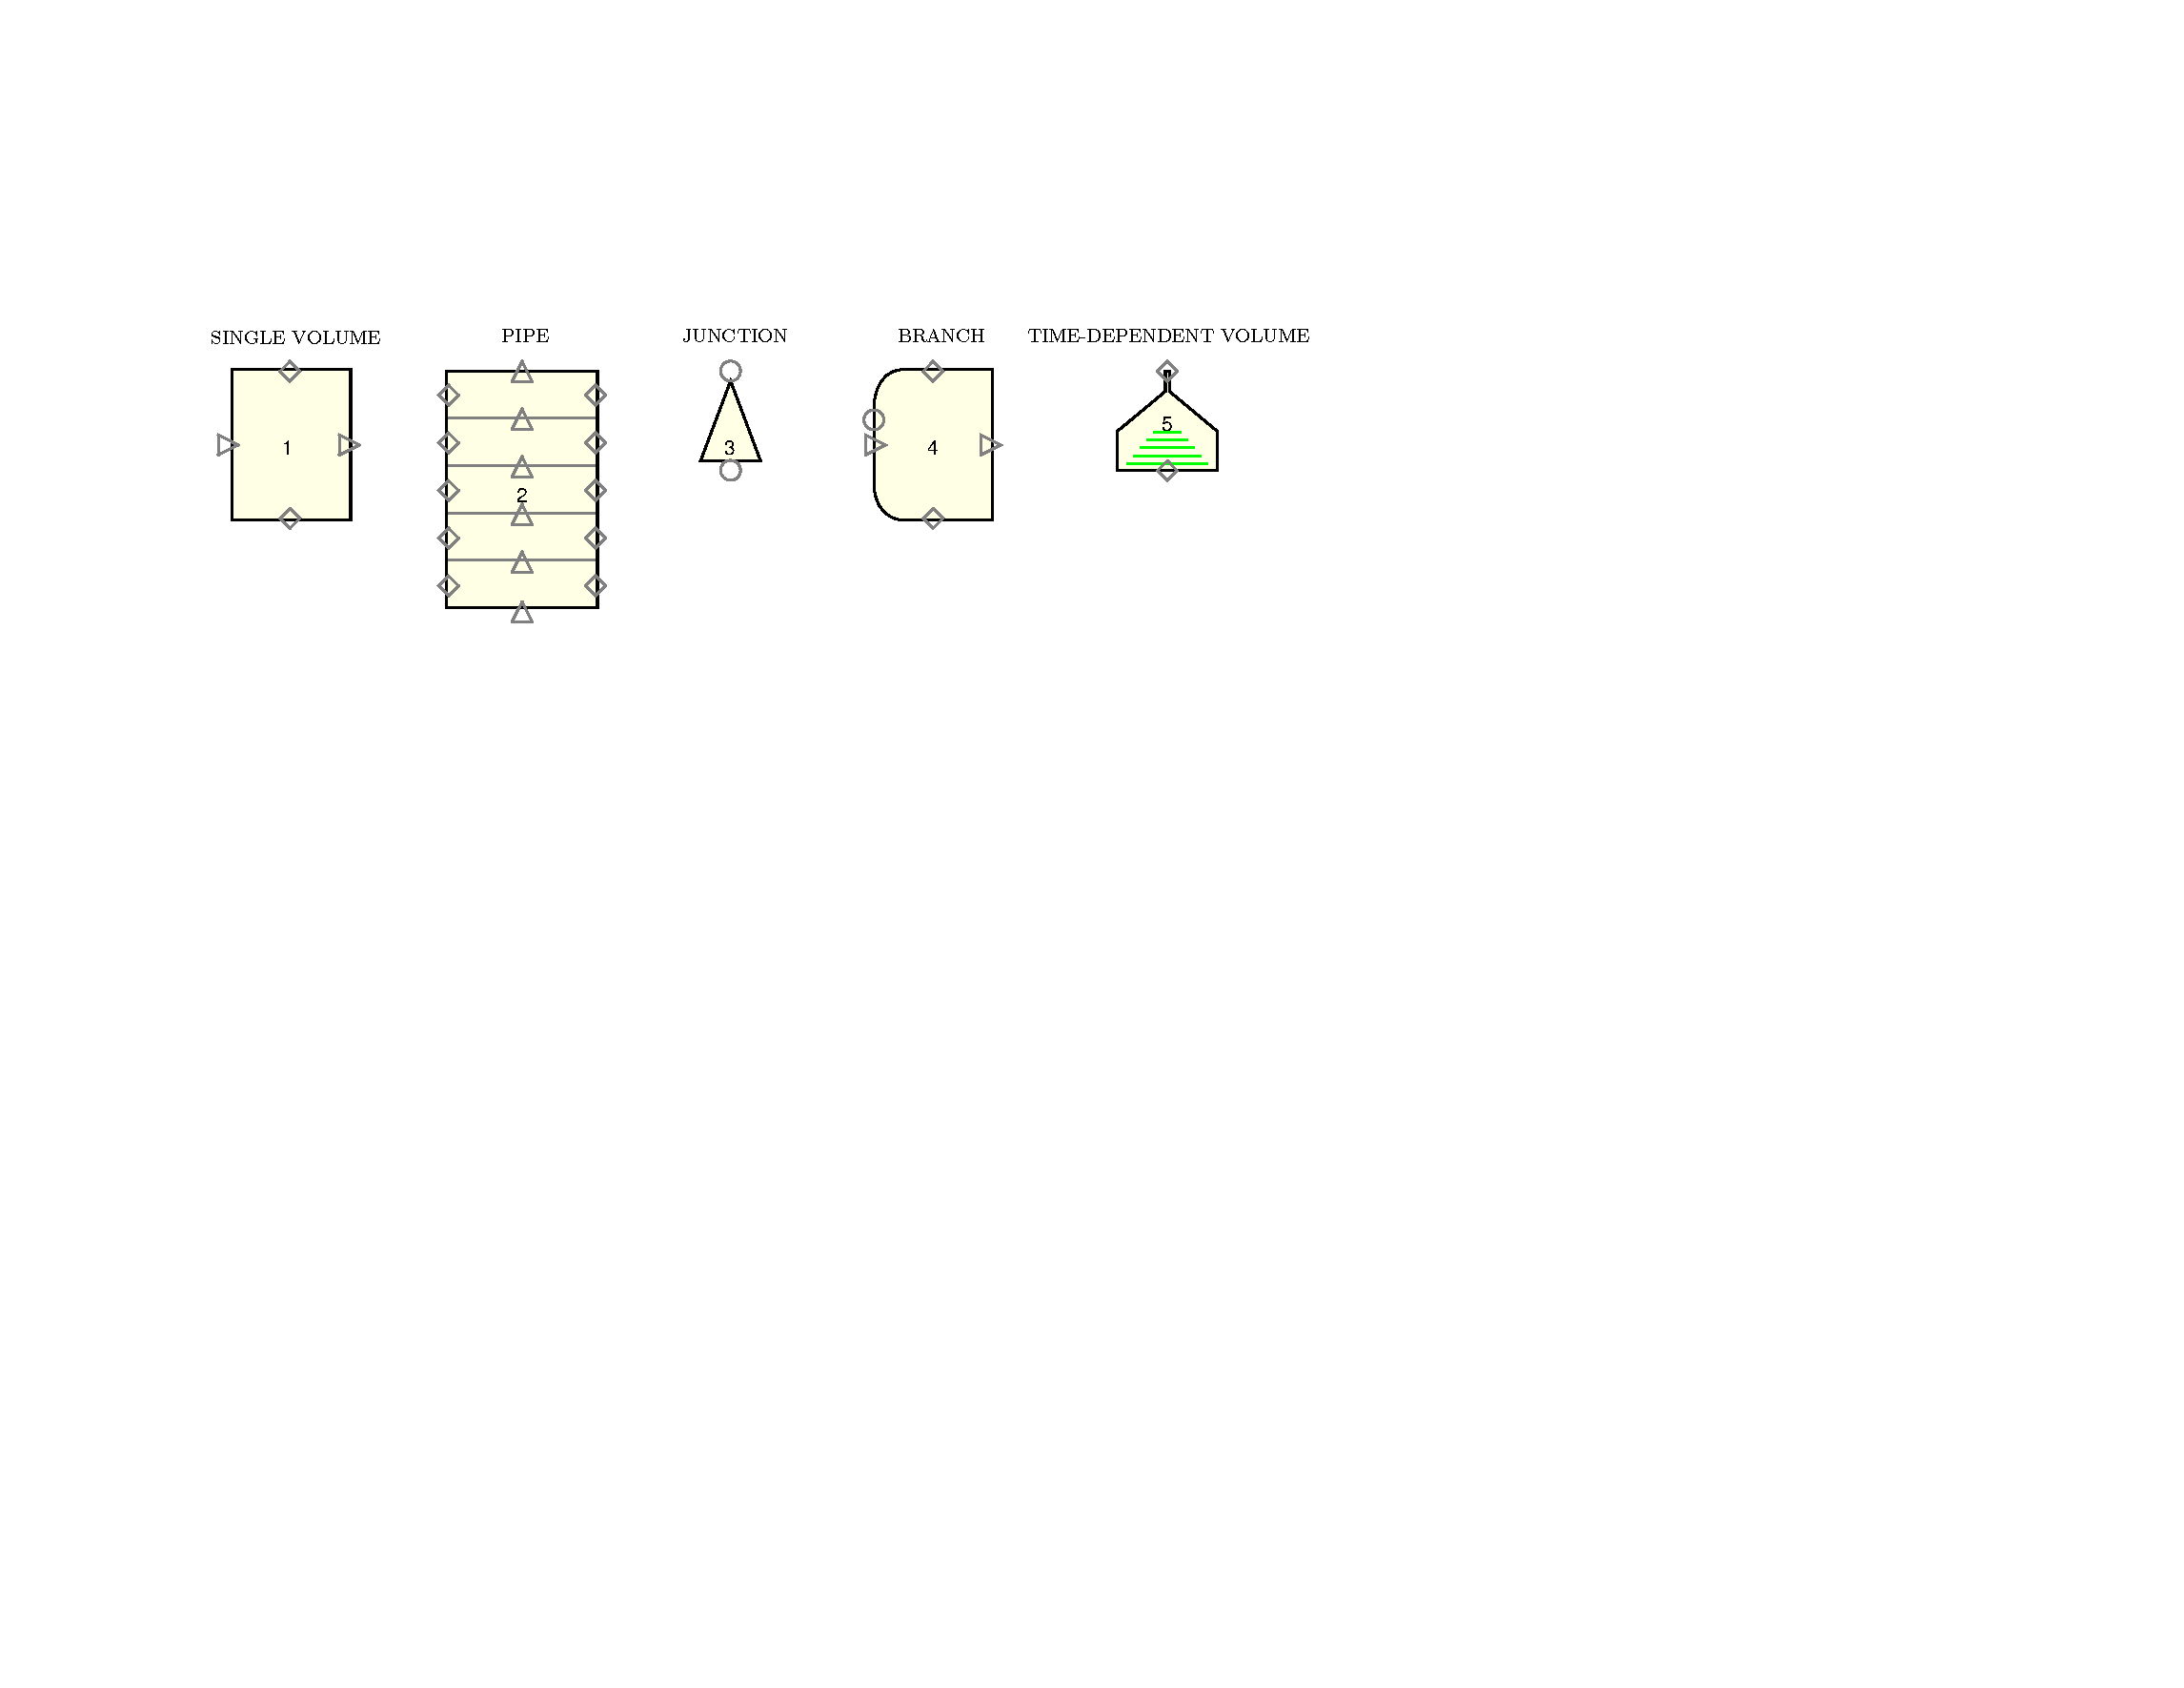
\includegraphics[clip, trim = 2cm 18cm 10cm 5cm, width=1.2\textwidth]{./03_benchmark/obrazky/HydraulicComponentsRELAPFinal.pdf}
	\caption{Hydraulické komponenty v programu RELAP5.}
	\label{fig:components_relap}
\end{figure}
Problematická se může jevit především nodalizace jednotlivých komponent a struktur. Využitím jemnějšího rozdělení je možné dosáhnout podrobnějšího popisu, avšak příliš jemná nodalizace může způsobit nestabilní výpočet a fyzikálně neodpovídající výsledky. Důvody proč příliš jemná nodalizace může být problematická jsou dva \cite{petruzzi2008thermal}:
\begin{itemize}
	\item velká část empirických vztahů zahrnutých do programu je získána z výpočtu s pevně danou nodalizací, což již z principu vede k rozdílným podmínkám,
	\item numerické simulace využívané v systémových kódech využívají uměle vloženou viskozitu za účelem získání stabilních výsledků.
\end{itemize}
Důležitým aspektem při popisu komplexního problému je propojení jednotlivých součástek, které může mít značný vliv na výsledné proudění. Pro nevhodně strukturovaných propojeních může docházet např. k různým obtokům, protiproudům či cirkulacím. Systémové kódy ve většině případů nabízejí model vytvořit z jednoduchých komponent, a proto je nutné při tvorbě modelu použít \uv{inženýrský odhad} a využít zkušenosti uživatele \cite{petruzzi2008thermal}. 

\section{Model v RELAP5}
Cílem této sekce je představit zjednodušený model experimentální sestavy popsané v \cite{zeitoun1994subcooled}.

Pro jednoduchost byly podmínky v testovací sekci experimentální smyčky simulovány rozdílem v tlaku na vstupu a výstupu trubky, konstantním objemovým, výkonem elektrického ohříváku a vstupní, resp. výstupní teplotou vody.  

 Vytvořený model je vyobrazen na Obr. \ref{fig:zeitoun_model},  modelované podmínky vycházející z \cite{zeitoun1994subcooled} jsou uvedeny v Tab. \ref{tab:zeitoun_podminky}. Tlak a teplota na vstupu byly nastaveny pomocí časově závislé objemové komponenty 1 (dále TDV), průtok byl nastaven časově závislou spojovací jednotkou 2 (dále TDJ) a tlak na výstupu komponentou TDV 9. Jelikož geometrie trubek je v programu RELAP5 značně omezená, k aproximaci průtočné trubky byla využita kruhová trubka s odpovídajícím hydraulickým průměrem $ d_h = 0,0127 $ m. Geometrie testovací trubice je vykreslena na Obr. \ref{fig:zeitoun_geometrie}. Průtočná plocha má tvar mezikruží s vnějším průměrem 25,4 mm a el. ohřívák tvar válce s průměrem 12,7 mm.
 \begin{figure}[h]
	\centering
	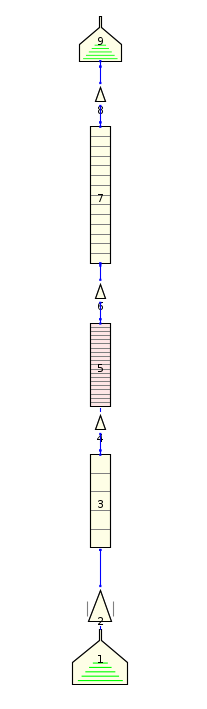
\includegraphics[width=0.3\textwidth]{./03_benchmark/obrazky/zeitoun_model.png}
	\caption{Termohydraulický model testovací trubice - RELAP.}
	\label{fig:zeitoun_model}
\end{figure}
\begin{table}[h]
	\centering
	\caption{Podmínky pro ověření modelu \cite{zeitoun1994subcooled}.}
	\label{tab:zeitoun_podminky}
	\begin{tabular}{cccccc}
		\hline
	experiment & P (W)            & G (kg/m$^2$s) & p$_{\text{in}}$ (kPa) & T$_{\text{in}}$ (K) & p$_{\text{out}}$ (kPa) \\
	\hline \hline
	BC1        & 2607 & 161,2      & 114         & 363,75    & 103,15    \\
	BC7        & 5869 & 208,05     & 114         & 356,65    & 103,15    \\
	BC9        & 5925 & 485,34     & 132         & 361,85    & 121,14   \\
	BC13       & 7366 & 348,94     & 137         & 361,15    & 126,13     \\ \hline
		\end{tabular}

	
\end{table}
\section{Výsledky experimentů a výpočtů}
Na Obr. \ref{fig:zeitoun_bc1}, \ref{fig:zeitoun_bc7}, \ref{fig:zeitoun_bc9} a \ref{fig:zeitoun_bc13} jsou vykresleny průběhy dutinového koeficientu v vyhřívané sekci testovací trubice. Ve všech případech je možné rozdělit oblasti na silně podchlazenou oblast (\uv{Highly subcooled region}) a slabě podchlazenou oblast (\uv{Low subcooling region}). Přechod mezi těmito regiony je nazýván \uv{Onset of significant void} a ve všech případech je situován ve výšce okolo 0,2 m \cite{KONCAR2003255}.  

Z Obr. \ref{fig:zeitoun_bc1}, \ref{fig:zeitoun_bc7}, \ref{fig:zeitoun_bc9} a \ref{fig:zeitoun_bc13} je jasně vidět, že zatímco ve vysoce podchlazené oblasti je dutinový koeficient menší ve srovnání s experimenty, tak v slabě podchlazené oblasti dává program RELAP5 nadhodnocené výsledky. Kvalitativně jsou ovšem výsledky ve shodě s měřením. Ve všech případech je přechod mezi výše zmíněnými oblastmi v okolí bodu 0,2 m, kdy dochází k výraznému nárůstu dutinového koeficientu. Důvodem nesrovnalostí může být jak jednak zjednodušený popis experimentální smyčky, tak extrapolace empirických vztahů odvozených pro vysoké tlaky. 

Při porovnání dutinového koeficientu vycházejícího z modelu \ref{fig:zeitoun_model} a výsledků z \cite{KONCAR2003255} lze pozorovat obdobné odchylky od experimentálních dat. Přestože se jedná o rozdílný model a rozdílnou verzi programu RELAP5, tak lze vytvořený model považovat za dostatečně přesný. 

\begin{figure}[p]
	\centering
	\begin{minipage}{.5\textwidth}
		\centering
		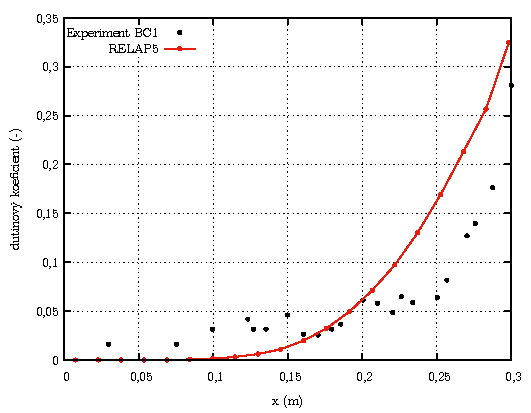
\includegraphics[width=\linewidth]{./03_benchmark/grafy/srovnani_exp1.pdf}
		\caption{Srovnání dutinového koeficientu - exp. BC1.}
		\label{fig:zeitoun_bc1}
	\end{minipage}%
	\begin{minipage}{.5\textwidth}
		\centering
		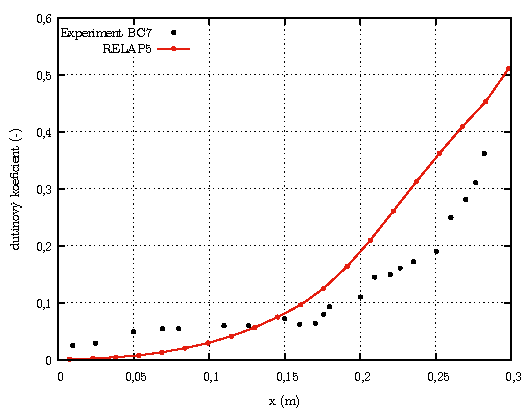
\includegraphics[width=\linewidth]{./03_benchmark/grafy/srovnani_exp2.pdf}
		\caption{Srovnání dutinového koeficientu - exp. BC7.}
		\label{fig:zeitoun_bc7}
	\end{minipage}
\end{figure}

\begin{figure}[p]
	\centering
	\begin{minipage}{.5\textwidth}
		\centering
		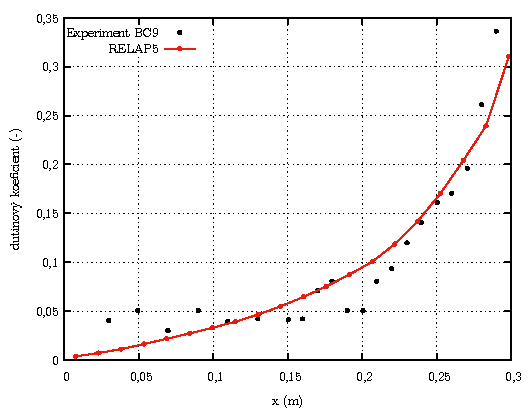
\includegraphics[width=\linewidth]{./03_benchmark/grafy/srovnani_exp3.pdf}
		\caption{Srovnání dutinového koeficientu - exp. BC9.}
		\label{fig:zeitoun_bc9}
	\end{minipage}%
	\begin{minipage}{.5\textwidth}
		\centering
		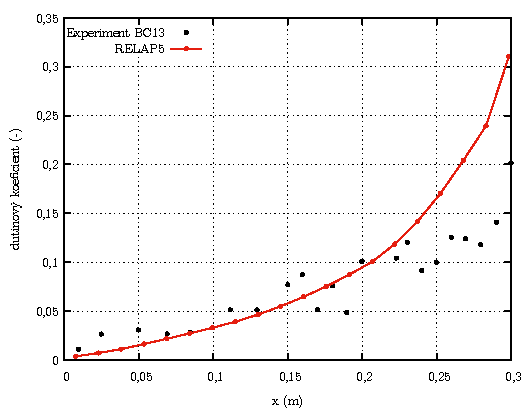
\includegraphics[width=\linewidth]{./03_benchmark/grafy/srovnani_exp4.pdf}
		\caption{Srovnání dutinového koeficientu - exp. BC13.}
		\label{fig:zeitoun_bc13}
	\end{minipage}
\end{figure}
\chapter{Termohydraulický model palivového článku IRT-4M}

Pro vytvoření termohydraulického modelu školního reaktoru VR-1 byl použit program RELAP5, přičemž samotná tvorba byla rozdělena do několika sekcí. Jelikož možnosti modelování různých geometrií jsou v programu RELAP5 značně omezené, pro správnou interpretaci a zachování fyzikálních dějů byl nejdříve vytvořen hydraulický model palivového článku IRT-4M při nuceném proudění, který byl následně zjednodušen do podoby sjednocené trubky. Poté byl vytvořen termohydraulický model, který interpretuje přirozené proudění v palivovém článku. Tento model byl následně opět zjednodušen a byl použit pro sestavení termohydraulického modelu reaktoru VR-1.

\section{Hydraulický model IRT-4M}
\label{sec:hydraulicky_model_irt}
Palivo IRT-4M je tvořeno 8, 6 nebo 4 koncentrickými čtvercovými trubkami se zakulacenými rohy s možností vložení vytěsnitele pro rovnoměrnější průtok. Geometrie a konstrukce použitá pro vytvoření modelu vychází z dokumentu \cite{sedlbauer2019}. Na Obr. \ref{fig:rad_irt_serpent} a \ref{fig:ax_irt_serpent} je vykreslen radiální a axiální průřez 8-trubkovým palivem bez vytěsnitele. Jelikož je geometrie trubek v programu RELAP5 omezená, tak jsou jednotlivé oddělené průtočné plochy aproximovány kruhovými trubkami s odpovídajícím hydraulickým průměrem. Komponenty 1-9 uvedené na Obr. \ref{fig:irt_hydraulic_relap} odpovídají průtočným plochám z \ref{fig:ax_irt_serpent}, plocha 10 pak představuje vytěsnitel (vstupní průměr vytěsnitele je 3 mm). Rozměry palivového článku a jednotlivých průtočných ploch jsou uvedeny v příloze v tab. \ref{tab:prilohy_irt_geometrie}. Nucené proudění bylo vytvořeno pomocí TDV 26 a 36 rozdílem v tlaku rovným 4 m vodního sloupce. Komponenty 22-25 a 32-35 představují koncovky a spojení jednotlivých trubek . Samotný hydraulický je ilustrován na Obr. \ref{fig:irt_hydraulic_relap} (pro lepší přehlednost není model v měřítku). 


\begin{figure}
	\centering
	\begin{minipage}{.5\textwidth}
		\centering{
		
\includegraphics[width=.8\textwidth, trim={40cm 40cm 40cm 40cm},clip]{./04_TH_model_IRT/obrazky/serpent_irt_hor_2.png}
		\caption{Radiální řez palivovým článkem IRT-4M.}
		\label{fig:rad_irt_serpent}
		\vspace{1pt}
		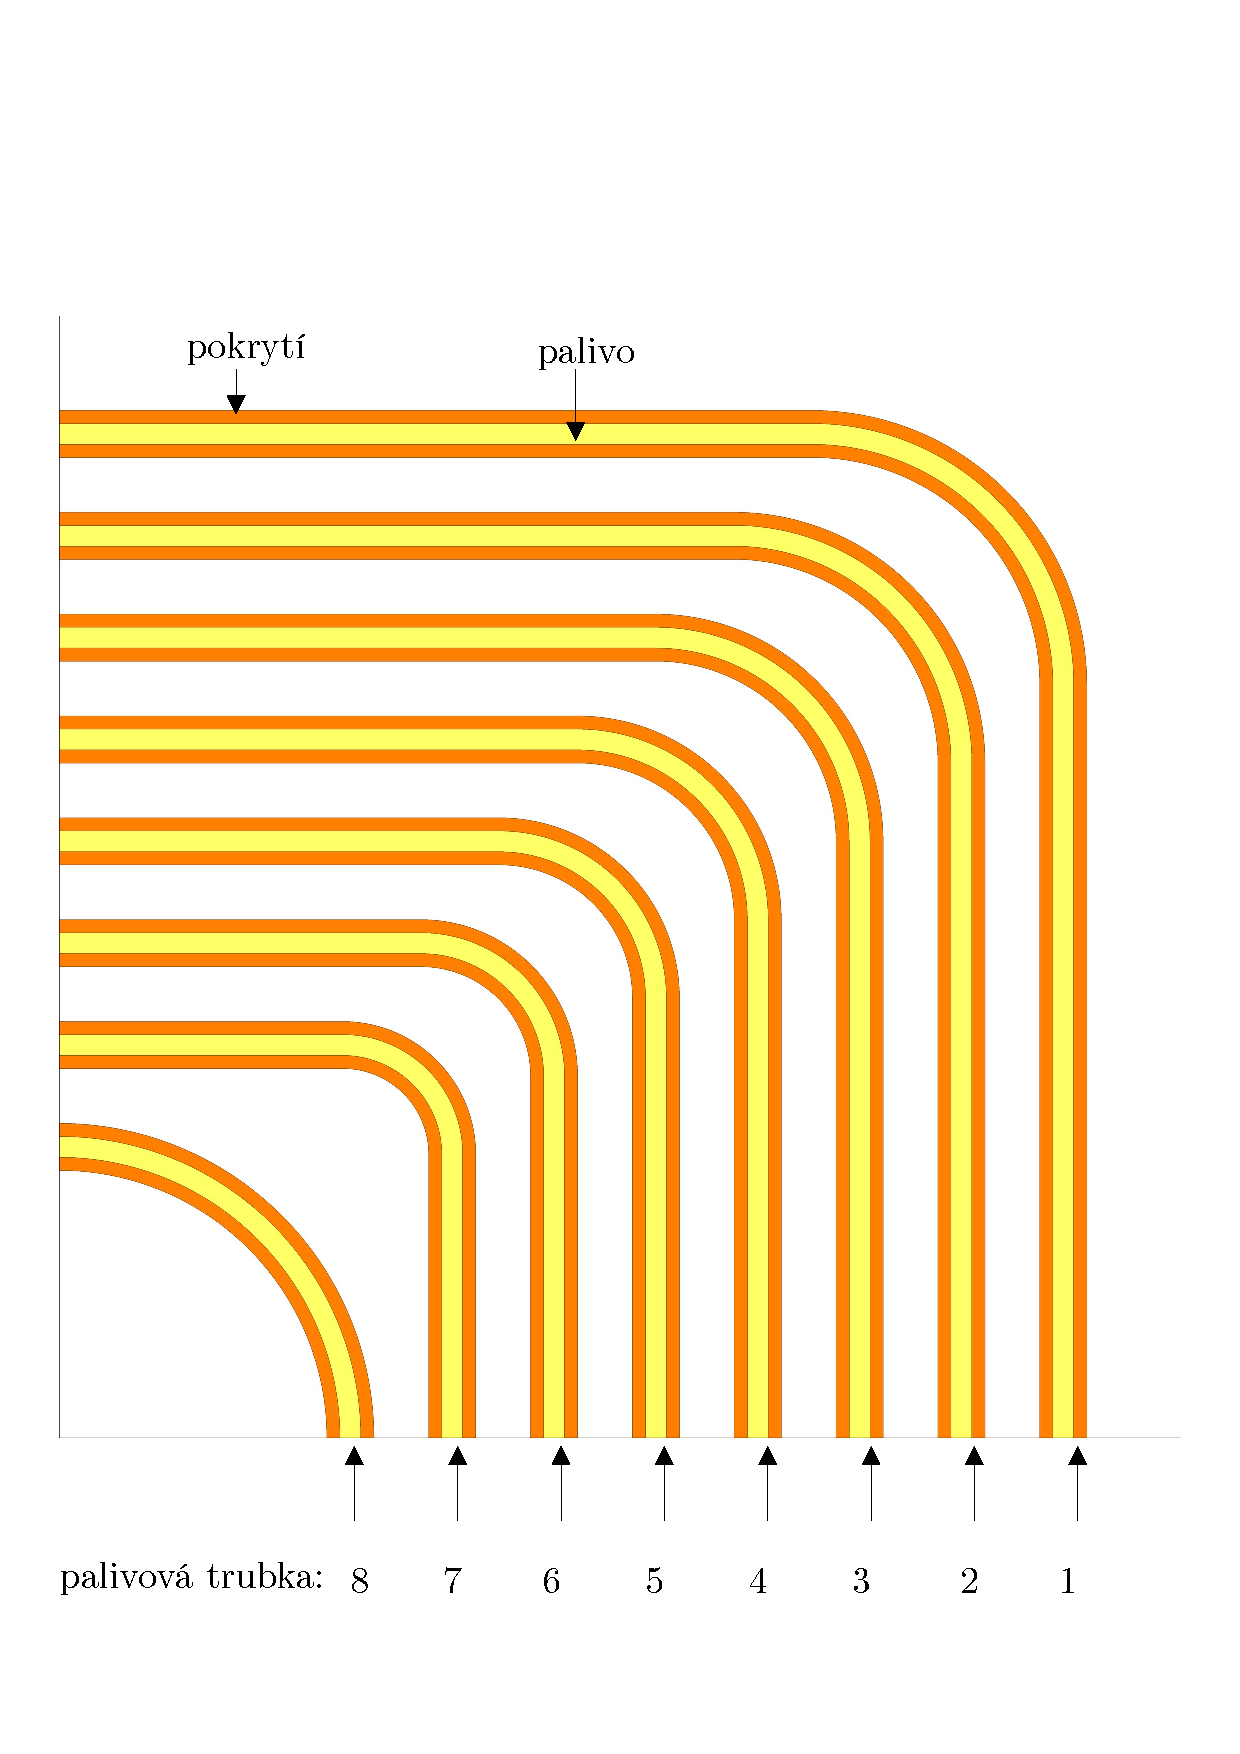
\includegraphics[width=.8\textwidth, trim={1.05cm 0cm 2cm 5.4cm},clip]{./04_TH_model_IRT/obrazky/serpent_irt_detail.pdf}
		\caption{Radiální řez palivovým článkem IRT-4M v detailu.}
		\label{fig:detail_irt_serpent}
	}
	\end{minipage}%
	\begin{minipage}{.5\textwidth}
		\centering
		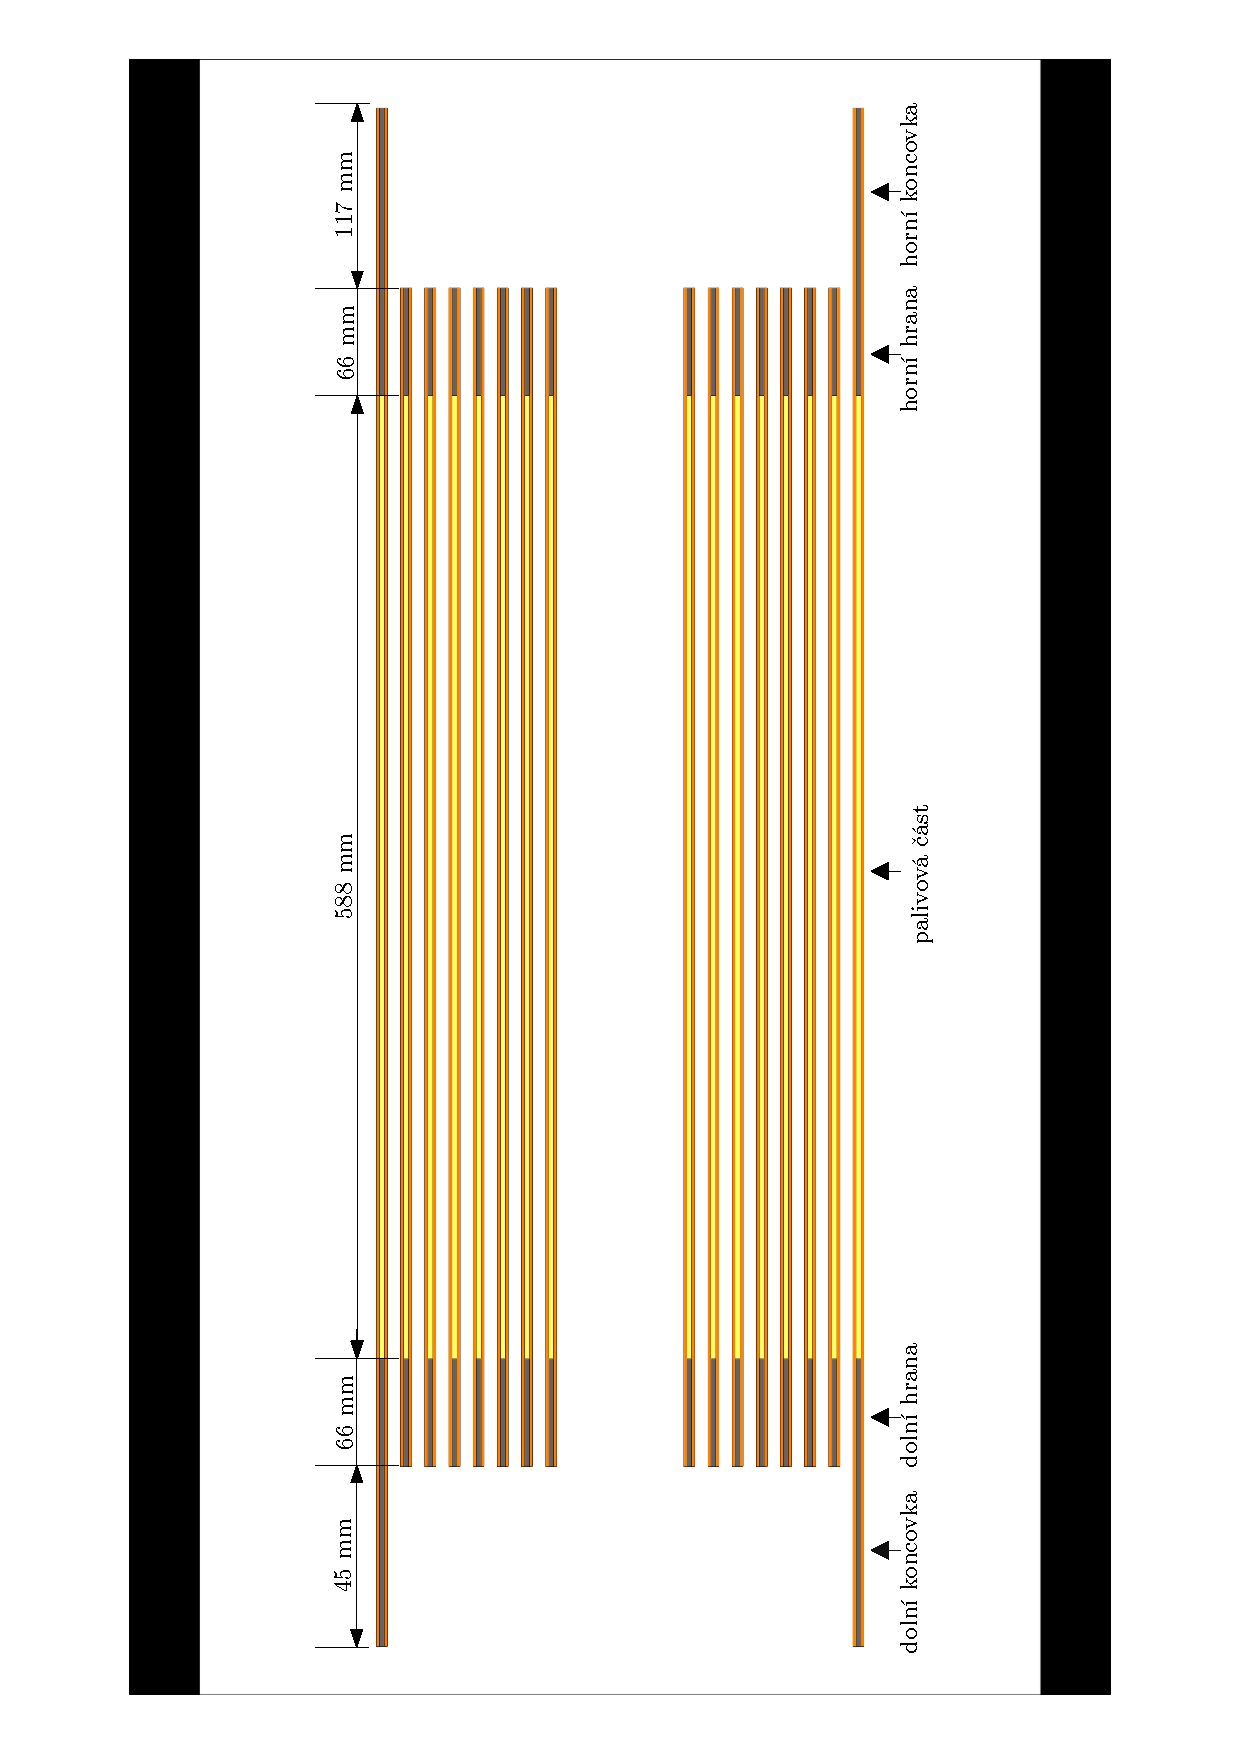
\includegraphics[width=.8\textwidth, trim={5cm 1.5cm 5cm 1.5cm},clip]{./04_TH_model_IRT/obrazky/serpent_irt_ver_2.pdf}
		\caption{Axiální řez palivovým článkem IRT-4M.}
		\label{fig:ax_irt_serpent}
	\end{minipage}
\end{figure}
\begin{figure}
	\centering
	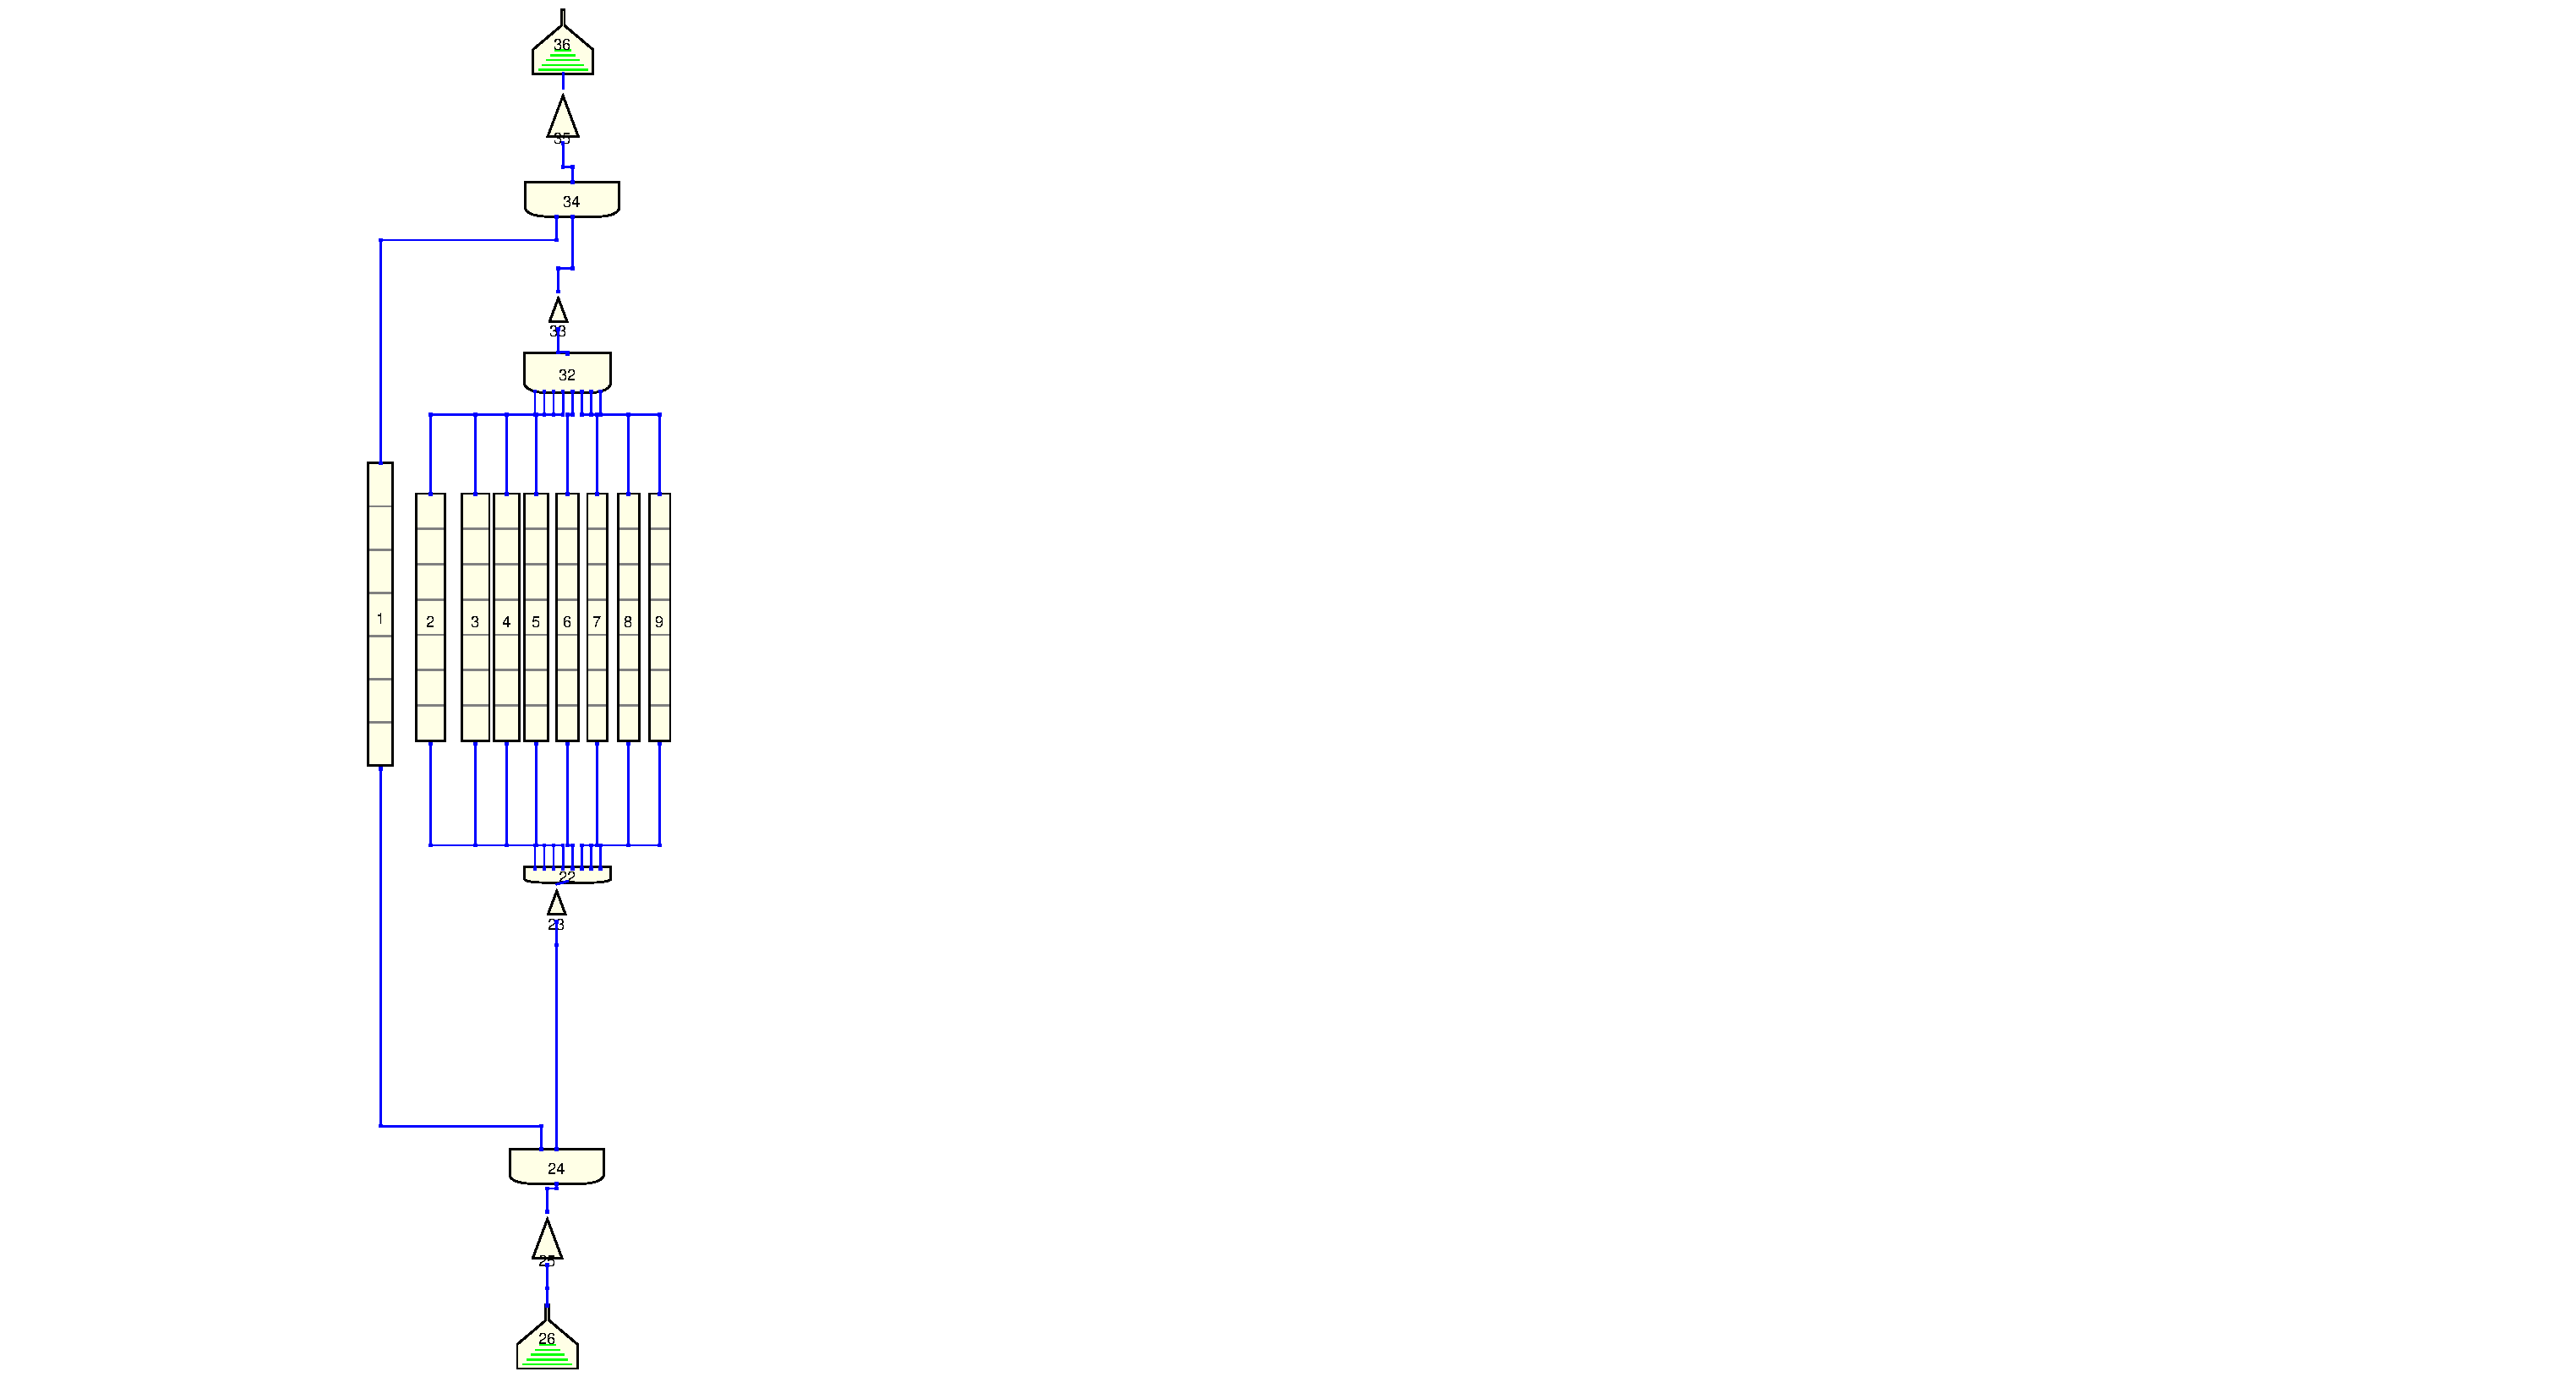
\includegraphics[width=0.6\textwidth, trim={5.5cm 0cm 35cm 0cm},clip]{./04_TH_model_IRT/obrazky/hydraulic_irt_relap.pdf}
	\caption{Hydraulický model palivového článku IRT-4M.}
	\label{fig:irt_hydraulic_relap}
\end{figure}
\newpage
\subsection{Ověření správnosti modelu}
Návrh a ověření modelu vyplývá z \cite{fejt}, kdy výsledné proudění je charakterizováno relativními objemovými průtoky $ G $ (m$ ^3/ $h) skrze průtočné plochy 1-10. Relativní průtoky G$ _i $/G (-) jsou uvedeny v Tab \ref{tab:rel_prutoky}. Celkový objemový průtok 8-trubkovým PČ v závislosti na tlakovém rozdílu vytvořeným odpovídajícím vodním sloupcem je v uveden tab. \ref{tab:celkovy_prutok_vodni_sloupec}. Pro srovnání byly použity výsledky uvedené v \cite{sedlbauer2019} (výsledky jsou označeny jako referenční). 
% Please add the following required packages to your document preamble:
% \usepackage[table,xcdraw]{xcolor}
% If you use beamer only pass "xcolor=table" option, i.e. \documentclass[xcolor=table]{beamer}
\begin{table}[H]
	\centering
	\caption{Relativní objemové průtoky skrze palivový článek (s odpovídajícím vytěsnitelem).}
	\label{tab:rel_prutoky}
	\resizebox{\textwidth}{!}{
		\begin{tabular}{ccccccc}
			\hline
			& \multicolumn{6}{c}{\textbf{G$_i$/G (-)}}   \\ \hline                                      
			Průtočná plocha & \multicolumn{2}{c}{\textbf{8-trubkový PČ}}                             & \multicolumn{2}{l}{\textbf{6-trubkový PČ}}                             & \multicolumn{2}{l}{\textbf{4-trubkový PČ}}                             \\ \hline \hline
			& RELAP5 & Referenční & RELAP5 & Referenční & RELAP5 & Referenční \\ \hline
			1               & 0,122 & 0,114 & 0,145 &0,130 & 0,182 & 0,173 \\
			2               & 0,165                         & 0,151                         & 0,194                         & 0,173                         & 0,243                         & 0,229                         \\
			3               & 0,147                         & 0,148                         & 0,174                         & 0,170                         & 0,218                         & 0,224                         \\
			4               & 0,130                         & 0,135                         & 0,153                         & 0,155                         & 0,192                         & 0,205                         \\
			5               & 0,112                         & 0,112                         & 0,132                         & 0,128                         & 0,166                         & 0,170                         \\
			6               & 0,095                         & 0,111                         & 0,112                         & 0,127                         &                               &                               \\
			7               & 0,077                         & 0,088                         & 0,091                         & 0,117                         &                               &                               \\
			8               & 0,115                         & 0,093                         & 0,000                         & 0,000                         &                               &                               \\
			9               & 0,035                         & 0,040                         &                               &                               &                               &                               \\
			10              & 0,003                         & 0,008                         &                               &                               &                               &                              \\ \hline
		\end{tabular}
	}
	
\end{table}



\begin{table}[H]
	\centering
	\caption{Celkový objemový průtok 8-trubkovým PČ (s vytěsnitelem).}
	\label{tab:celkovy_prutok_vodni_sloupec}
	\begin{tabular}{ccc}
		\hline
		$ \Delta  $p (m) & \multicolumn{2}{c}{\textbf{G} (m$ ^3 $/h)} \\ \hline
		& RELAP5 & Referenční \\ 
		\hline \hline
		2,45 & 22,7 & 25,6 \\
		3 & 27,5 & 28,4 \\
		3,5 & 31,3 & 30,7 \\
		4 & 34,8 & 32,8 \\ \hline
		
	\end{tabular}
	
\end{table}
\begin{table}[H]
	\centering
	\caption{Rozložení rychlostí v kanálech 8-trubkového PČ (s vytěsnitelem).}
	\label{tab:rel_rychlosti}
	\begin{tabular}{ccc}
		\hline
		& \multicolumn{2}{c}{\textbf{w }/ \textbf{w}$_{\text{max}} $} \\ \hline
		Průtočná plocha & RELAP5      & Referenční \\ \hline \hline
		1               & 0,81            & 0,84       \\
		2               & 0,77            & 0,78       \\
		3               & 0,77            & 0,86       \\
		4               & 0,77            & 0,89       \\
		5               & 0,77            & 0,86       \\
		6               & 0,77            & 1,00       \\
		7               & 0,77            & 0,98       \\
		8               & 1,00            & 0,90       \\
		9               & 0,78            & 0,98       \\
		10              & 0,05            & 0,18		\\ \hline      
	\end{tabular}
	
\end{table}
\begin{figure}[H]
	\centering
	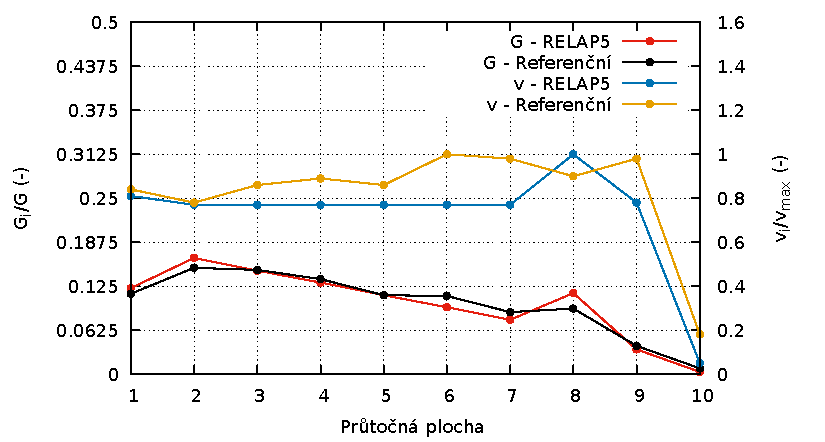
\includegraphics[width=\textwidth]{./04_TH_model_IRT/grafy/rozdeleni_v_g.pdf}
	\caption{Průtok a rychlost v jednotlivých kanálech.}
	\label{fig:rozdeleni_v_g}
\end{figure}
Na Obr. \ref{fig:rozdeleni_v_g} je vykresleno rozdělení relativních průtoků a rychlostí pro 8-trubkový palivový článek s vytěsnitelem. Model vytvořený v RELAP5 dává větší rozdíly v průtocích, rozdělení rychlostí dává naopak rovnoměrnější hodnoty. Odchylky od referenčních hodnot mohou být způsobeny mnoha faktory a naprostá shoda se nedala očekávat. Tyto odchylky ovšem nemají pro další výpočty zásadní vliv a model může být považován za vhodný.

\section{Zjednodušený hydraulický model}
\label{sec:zjednoduseny_hydraulicky_model_irt}
V aktivní zóně reaktoru VR-1 je okolo 16 palivových článků, což dává okolo 160 průtočných kanálů (při uvažování 8-trubkových PČ S vytěsnitelem) pro celý model reaktoru. Pro lepší použitelnost modelu při výpočtech obsahujících externí 3D kinetiku je vhodnější vytvořit zjednodušený model palivového článku se sjednoceným kanálem (viz Obr. \ref{fig:irt_hydraulic_simple_relap}). Při sjednocení kanálů je třeba zachovat celkovou průtočnou plochu a získat adekvátní hydraulický průměr, který zaručí stejný průtok. Prvním odhad hydraulického průměru vychází z rovnice:
\begin{equation}
	d_h = \frac{4S}{o},
	\label{eq:dh}
\end{equation}
kde $S$, resp. $o$ je celková průtočná plocha, resp. celkový omočený obvod palivového článku. Následně byl průměr iterován pro získání průtoku z komplexního modelu viz Obr. \ref{fig:iterated_dh}. Zjednodušený hydraulický model PČ uvedený na Obr. \ref{fig:irt_hydraulic_simple_relap} je v následujících kapitolách využit k vytvoření termohydraulického \uv{jednotkového} modelu (viz sekce \ref{sec:termohydraulicky_model}), který představuje PČ v modelu reaktoru VR-1.

\begin{figure}
	\centering
	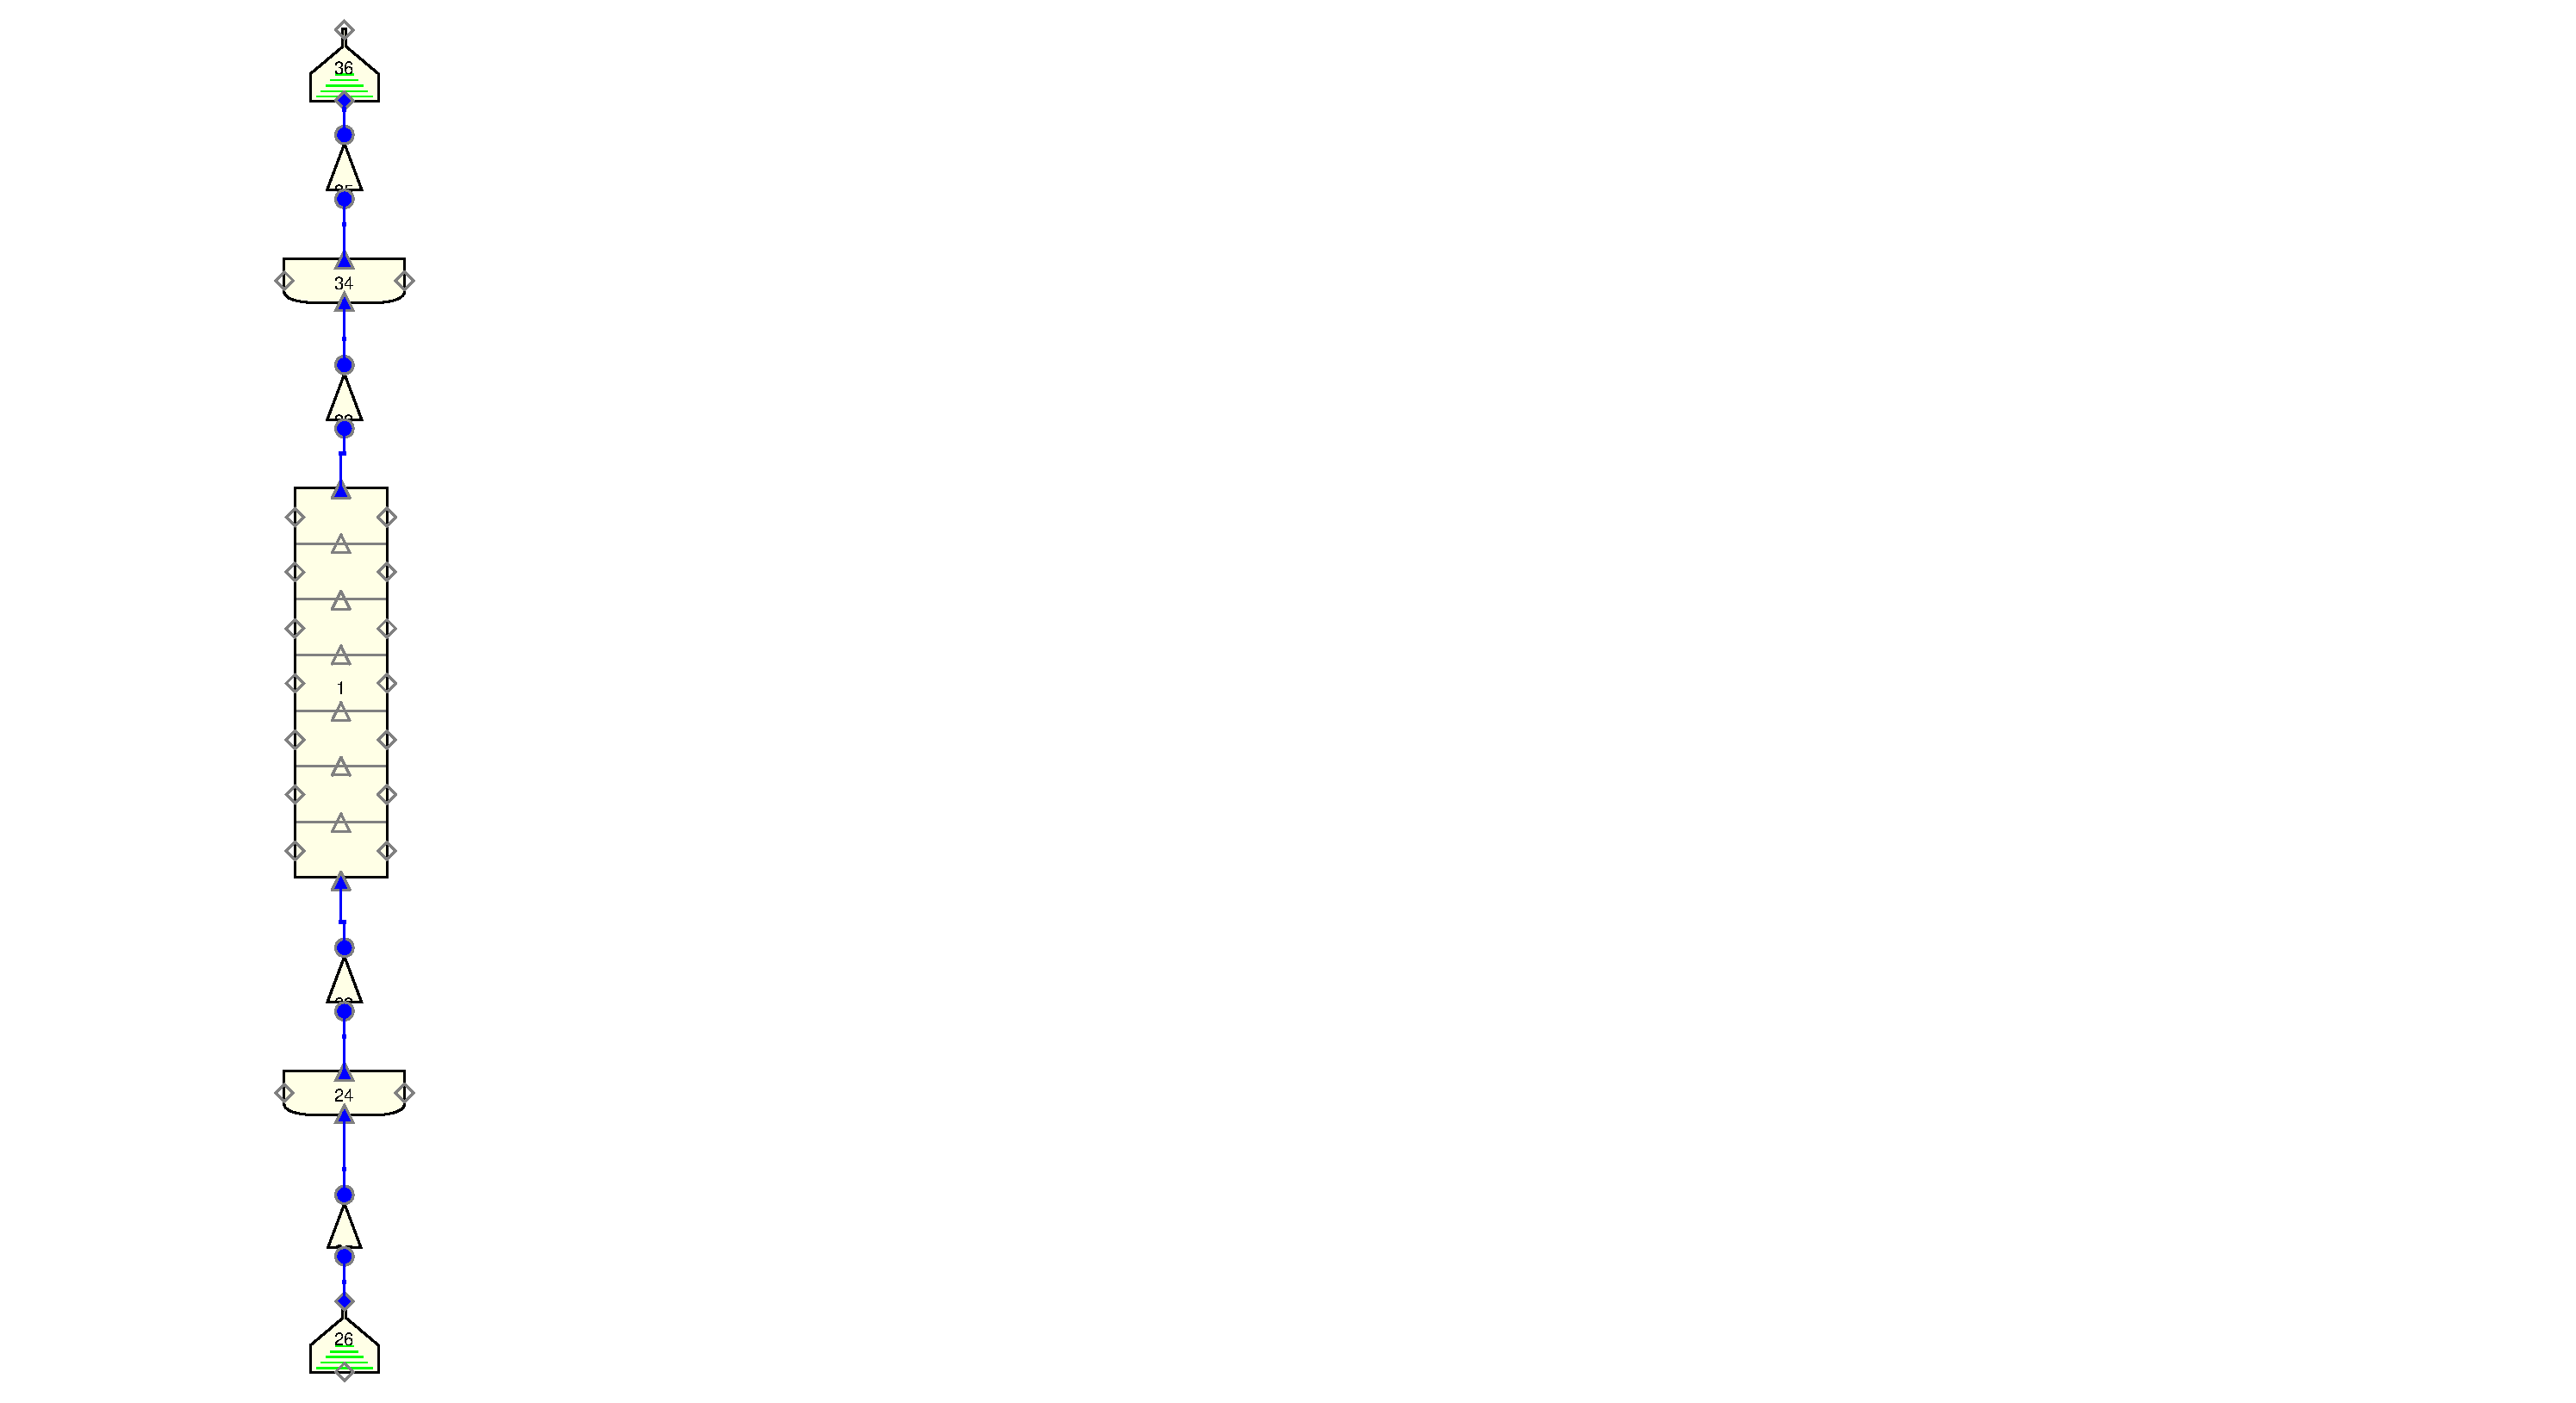
\includegraphics[width=0.6\textwidth, trim={0cm 0cm 39cm 0cm},clip]{./04_TH_model_IRT/obrazky/hydraulic_irt_simple_relap.pdf}
	\caption{Zjednodušený hydraulický model palivového článku IRT-4M.}
	\label{fig:irt_hydraulic_simple_relap}
\end{figure}
\subsection{Ověření správnosti modelu}
Závislost průtoku na hydraulickém průměru zjednodušeného modelu je vykreslena na Obr. \ref{fig:iterated_dh}. Rozdíl tlaku $\Delta p$ odpovídá 4 metrům vodního sloupce.
\begin{figure}[H]
	\centering
	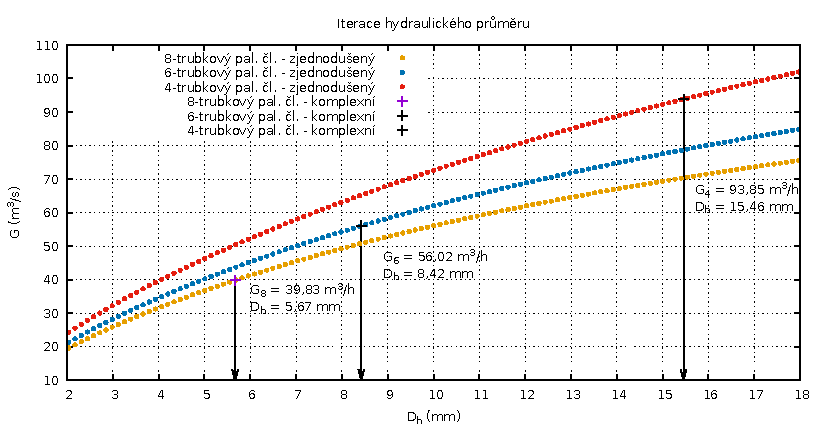
\includegraphics[width=\textwidth]{./04_TH_model_IRT/grafy/extrapolace_dh.pdf}
	\caption{Závislost průtoku skrz PČ (bez vytěsnitele) na hydraulickém průměru.}
	\label{fig:iterated_dh}
\end{figure}
V Tab. \ref{tab:prutoky_it_srovnani} jsou uvedeny získané hydraulické průměry s odpovídajícím průtokem.
\begin{table}[H]
	\centering
	\caption{Průtok v komplexním a zjednodušeném modelu PČ (bez vytěsnitele) pro různé hydraulické průměry. }
	\label{tab:prutoky_it_srovnani}
	\begin{tabular}{cccc}
		\hline
		& \textbf{G} (m$^3$/h) - komplex. & \textbf{G} (m$^3$/h) - rovnice \ref{eq:dh} & $d_h$ (mm) - rovnice \ref{eq:dh} \\
		\hline \hline
		4-trubkový PČ & 93,85  & 65,70 & 8,52 \\
		6-trubkový PČ & 56,02  & 43,73 & 5,68 \\
		8-trubkový PČ & 39,83  & 34,68 & 4,59 \\
		\hline
		&&&\\
		&&&\\
		\hline 
		& \textbf{G} (m$^3$/h) - komplex.& \textbf{G} (m$^3$/h) - iterace & $d_h$ (mm) - iterace  \\
		\hline \hline
		4-trubkový PČ & 93,85  & 93,85 & 15,46 \\
		6-trubkový PČ & 56,02  & 56,02 & 8,42 \\
		8-trubkový PČ & 39,83  & 39,84 & 5,67 \\
		\hline 

	\end{tabular}

\end{table}	
Cílem sekce \ref{sec:hydraulicky_model_irt} a \ref{sec:zjednoduseny_hydraulicky_model_irt} bylo vytvoření hydraulického modelu, který je použitelný pro model reaktoru VR-1. Nejzásadnějším krokem popsaným v těchto kapitolách je sjednocení průtočných kanálů, které by mělo zajistit vhodnou strukturu pro následující výpočty. Iterací hydraulického průměru bylo dosaženo identického průtoku a je možné považovat zjednodušený hydraulický model za dostatečný.
\newpage

\section{Termohydraulický model PČ IRT-4M}
\label{sec:termohydraulicky_model}
V předchozí sekci byl prezentován model PČ, ve kterém docházelo k nucenému proudění určeného rozdílem v tlaku na okrajích rozhraní. Tyto okrajové podmínky byly zajištěny párem TDV. Problém je, že školní reaktor VR-1 je charakteristický odvodem tepla za pomocí přirozeného proudění a je nutné vytvořit model, který tuto skutečnost bude respektovat a co nejlépe popisovat. Z \cite{fejt} vyplývá, že kromě vhodně zvolených komponent je třeba také zvolit sledované fyzikální veličiny pro co nejvíce přesnou interpretaci a srovnání výsledků.

Při srovnání Obr. \ref{fig:irt_hydraulic_relap} a \ref{fig:irt_nat_conv_komplex} lze vidět, že pár TDV byl zaměněn za smyčku složenou z trubek a spojovacích komponent, která představuje obtok okolo PČ. Výška vertikálního kruhové trubky obtoku byla nastavena na 3,555 m a její průměr na 2,3 m, což zhruba odpovídá geometrii reaktorové nádoby. Dále byl ke komponentě 53 připojena TDV simulující otevřenou vodní hladinu při atmosférickém tlaku (p = 101,325 kPa, T = 293 K). V případě komplexního, resp. zjednodušeného modelu byla pro samotný PČ převzata již vytvořená geometrie viz \ref{fig:irt_hydraulic_relap}, resp. \ref{fig:irt_hydraulic_simple_relap}, přičemž konstrukce obtoku zůstává pro obě dvě varianty modelu stejná.

Hlavním problémem při zadávání zdrojů tepla bylo vystihnutí správné geometrie. Jelikož průřez trubkou PČ IRT-4M odpovídá čtverci s kulatými rohy (viz Obr. \ref{fig:rad_irt_serpent}) a geometrie zdrojů tepla (HS) v RELAP5 je značně omezená, musely být jednotlivé trubky napodobeny válcovou geometrií s vnějším a vnitřním průměrem. Tyto parametry byly získány z podmínek na identický objem, teplosměnnou plochu a tloušťku trubek viz \cite{fejt}. Rozměry jednotlivých HS komponent jsou uvedeny v tabulce \ref{tab:equivalent_hs}. Při přechodu z komplexního na zjednodušený model je třeba ověřit zachování fyzikálních veličin \cite{fejt}: 
\begin{itemize}
	\item velikost průtoku skrze PČ vlivem přirozené konvekce,
	\item výstupních teplot,
	\item výskyt varu.
\end{itemize}
Pro ohřev vody v PČ můžeme předpokládat následující zjednodušený vztah:
\begin{equation}
	\Delta T_{cool} = \frac{Q}{\rho \text{ G } c_p } = \frac{Q}{\rho \text{ w } A \,c_p },
\end{equation}
kde Q (W) je tepelný výkon, $\rho$ (kg/m$^3$) je hustota, $c_p$ (J/kg$\cdot$K) měrná tepelná kapacita a A (m$^2$) je průtočná plocha. Pro termohydraulický model bude uvažováno rovnoměrné rozložení výkonu  a rozložení výkonu vycházející z programu Serpent2. Jelikož je celkový výkon pro obě rozdělení totožný, je očekávatelné, že i celkový průtok bude velice podobný. Největší rozdíly se dají očekávat v rozdělení teplot a tudíž i možném výskytu varu.

\begin{table}[H]
	\centering
	\caption{Rozměry ekvivalentních HS pro PČ IRT-4M a jejich napojení na jednotlivé trubky (viz Obr. \ref{fig:irt_nat_conv_komplex} a \ref{fig:irt_nat_conv_jedno}). }
	\label{tab:equivalent_hs}
	\begin{tabular}{ccccccc}
		\hline
		HS &  &  & \multicolumn{2}{c}{Komplexní model} & \multicolumn{2}{c}{Zjednodušený model} \\
		 & $ r_i $ (mm)& $ r_o $ (mm) & $V_i$ & $V_o$ & $V_i$ & $V_o$ \\
		 \hline
		 \hline
		
		1 & 40,17 & 41,77 & 22 & 21 & 11 & 11 \\
		2 & 35,99 & 37,59 & 23 & 22 & 11 & 11 \\
		3 & 31,82 & 33,42 & 24 & 23 & 11 & 11 \\
		4 & 27,65 & 29,25 & 25 & 24 & 11 & 11 \\
		5 & 23,47 & 25,07 & 26 & 25 & 11 & 11 \\
		6 & 19,30 & 20,90 & 27 & 26 & 11 & 11 \\
		7 & 15,12 & 16,72 & 28 & 27 & 11 & 11 \\
		8 & 9,05  & 10,65 & 29 & 28 & 11 & 11  \\
		
		\hline
	\end{tabular}
\end{table}

\begin{figure}[H]
	\centering
	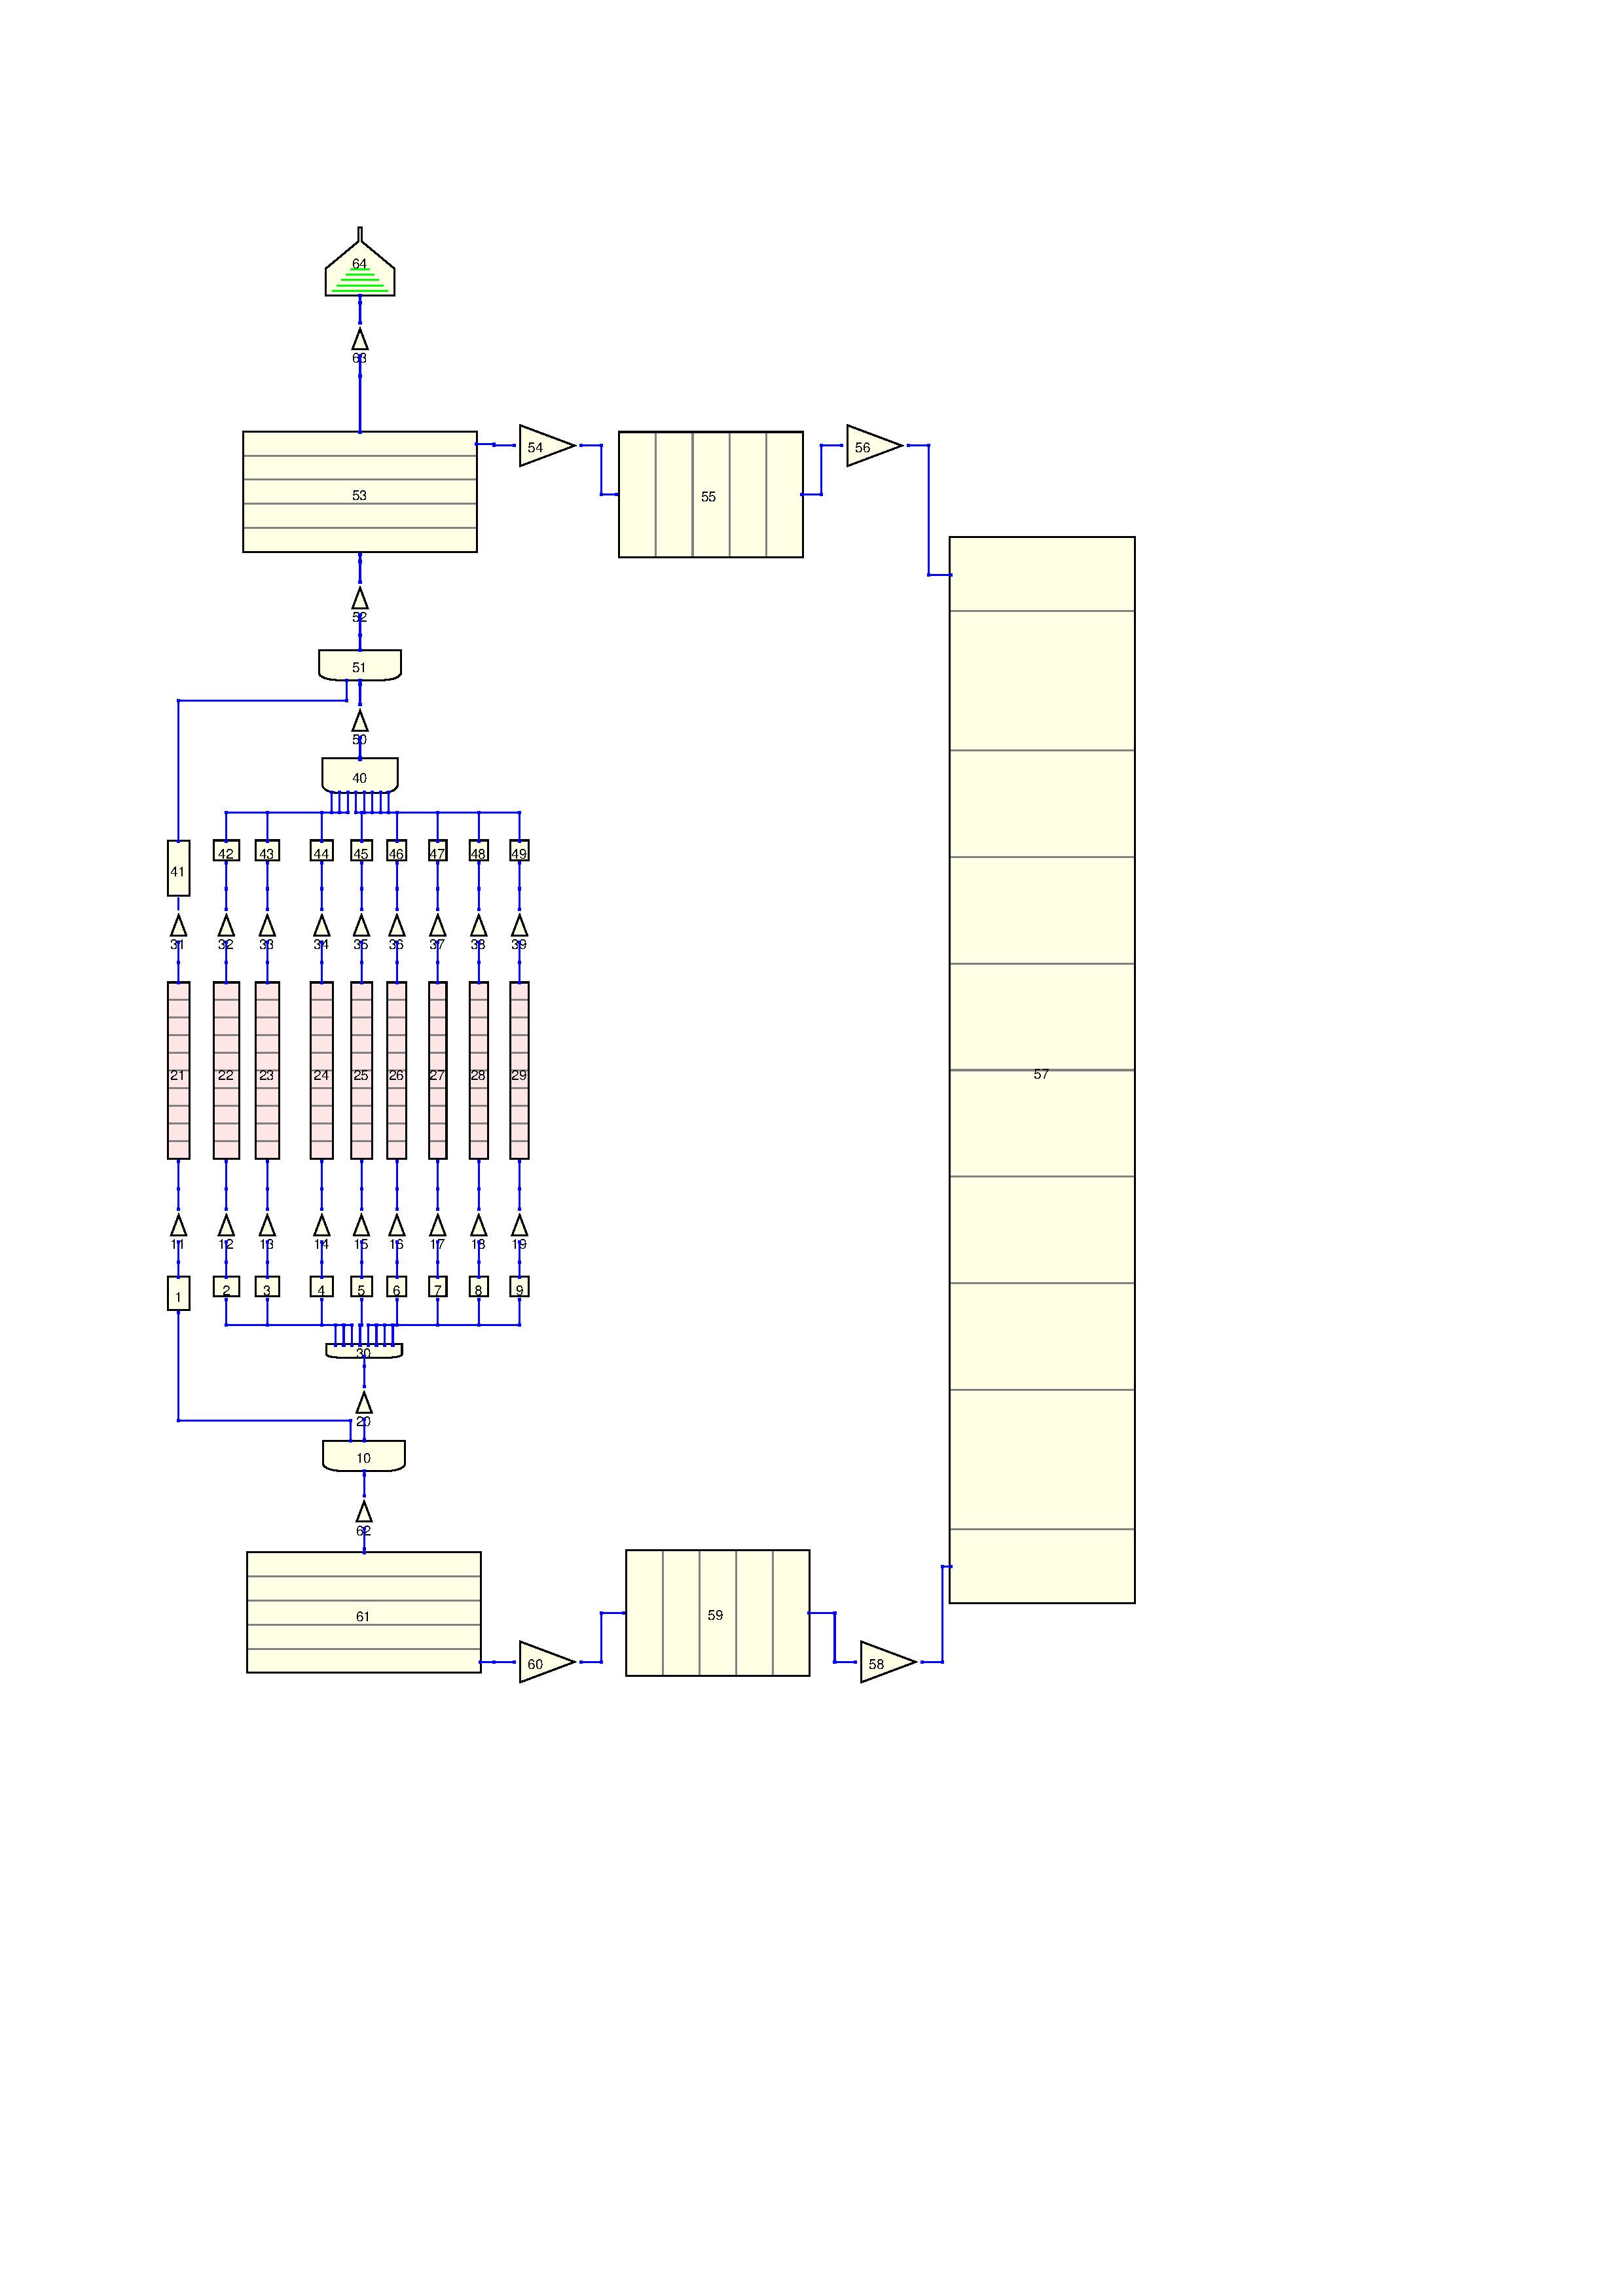
\includegraphics[width=\textwidth, trim={4cm 15cm 12cm 6cm}, clip]{./07_prilohy/prehled_modelu/t8bk.pdf}
	\caption{Termohydraulický komplexní model 8-trubkového PČ IRT-4M bez vytěsnitele (Pro lepší vizualizaci byly měřítka komponent 53 až 62 změněna).}
	\label{fig:irt_nat_conv_komplex}
\end{figure} 
\begin{figure}[H]
	\centering
	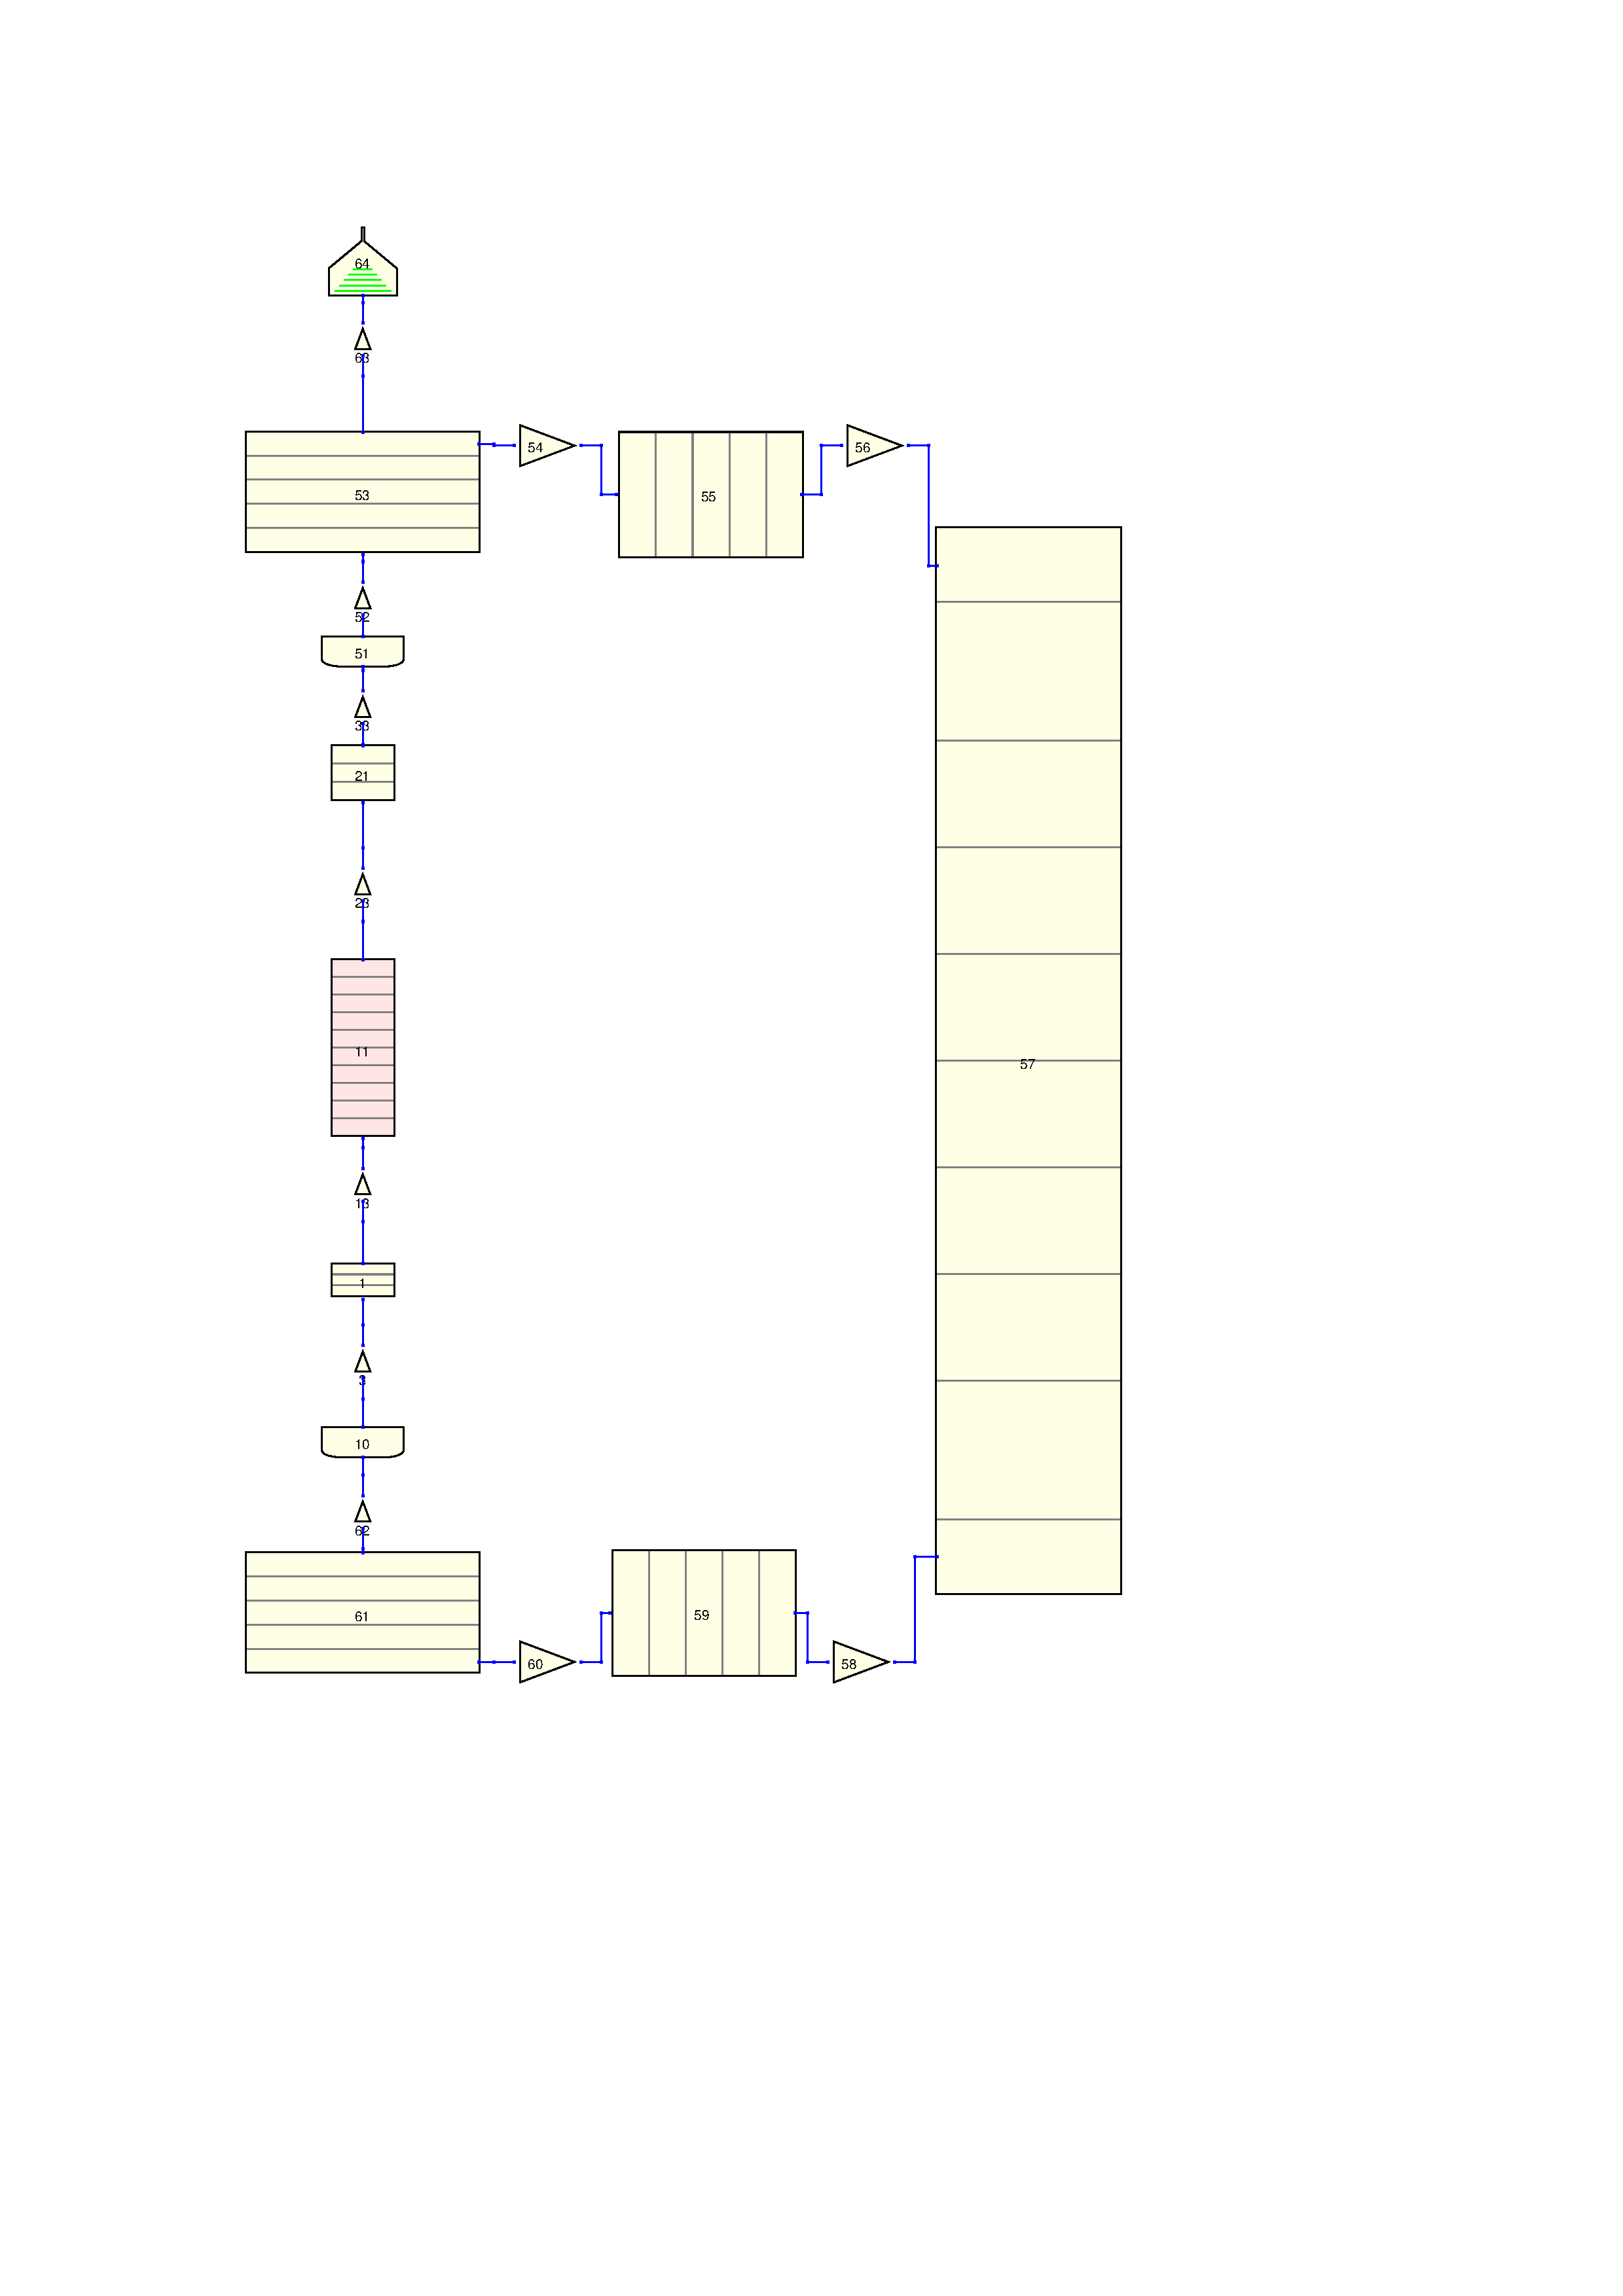
\includegraphics[width=\textwidth, trim={4cm 15cm 12cm 6cm}, clip]{./07_prilohy/prehled_modelu/t8bj.pdf}
	\caption{Termohydraulický zjednodušený model 8-trubkového PČ IRT-4M bez vytěsnitele (Pro lepší vizualizaci byly měřítka komponent 53-62 změněna).}
	\label{fig:irt_nat_conv_jedno}
\end{figure}

Pro vytvoření zdroje tepla v PČ byla uvažována dvě rozložení výkonu, a to rovnoměrné rozdělení a distribuce výkonu dle výpočetního programu Serpent2. V obou případech byl studován průtok, ohřev a výskyt povrchového bublinkového varu při přechodu z komplexního na zjednodušený model. Celkový výkon byl nastaven na 1,5$ \cdot 10^5$ W, přičemž pro rovnoměrné rozdělení se předpokládal zlomek výkonu v každém nódu 0.0125 (8 trubek, v každé 10 nódů), tedy každý nód produkuje 1875 W. Rozložení výkonu z programu Serpent2 je uvedeno v tab. \ref{tab:rozlozeni_vykonu_irt_serpent} a na Obr. \ref{fig:rozlozeni_vykonu_irt_serpent}.
\begin{table}[H]
	\centering
	\caption{Rozložení výkonu v 8-trubkovém PČ IRT-4M dle programu Serpent.}
	\label{tab:rozlozeni_vykonu_irt_serpent}
	\begin{tabular}{cc|cc}
		\hline
		Nód (-) & $P_{\text{rel}}^{\text{ax}}$ (-) & Palivová trubka & $P_{\text{rel}}^{\text{trubka}}$ (-) \\
		\hline \hline
		10 & 0,053 &  1& 0,22 \\
		9  & 0,081  & 2& 0,18 \\
		8  & 0,108  & 3& 0,15 \\
		7  & 0,126  & 4& 0,13 \\
		6  & 0,135  & 5& 0,11 \\
		5  & 0,135  & 6& 0,09 \\
		4  & 0,125  & 7& 0,08 \\
		3  & 0,106  & 8& 0,05 \\
		2  & 0,080  & &  \\
		1  & 0,052  & & \\
		\hline 
		
		
		
		
		
		
		
		
		
	\end{tabular} 
\end{table} 
\begin{figure}[H]
	\centering
	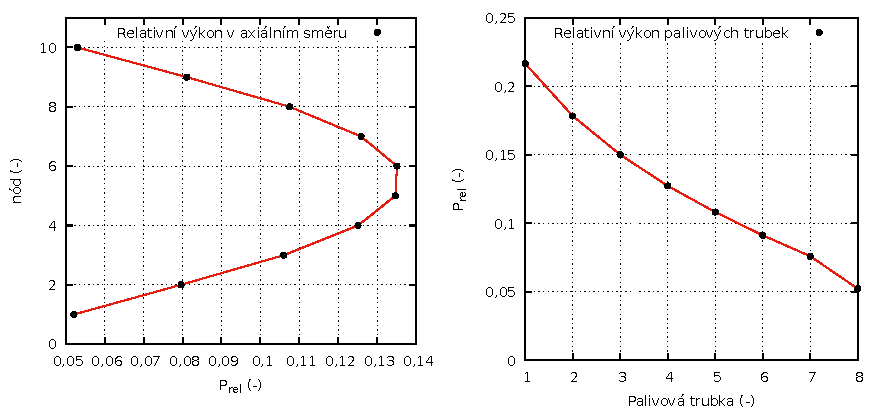
\includegraphics[width=0.8\textwidth]{./04_TH_model_IRT/grafy/average_power_distribution.pdf}
	\caption{Axiální a radiální rozložení výkonu v 8-trubkovém PČ IRT-4M - Serpent2.}
	\label{fig:rozlozeni_vykonu_irt_serpent}
\end{figure}
Axiální nodalizace palivových trubek v programu Serpent byla uvažována ve shodě s nodalizací trubek 21-29  viz Obr. \ref{fig:irt_nat_conv_komplex}, resp. trubky 11 viz Obr. \ref{fig:irt_nat_conv_jedno}. 

%V axiálním směru byla každá HS rozdělena na 10 nódů, přičemž zlomek celkového výkonu každé palivové trubky byl odlišný.  

\section{Sjednocení průtočných kanálů}
\label{sec:termohydraulicky_model_IRT}
Cílem následujícího textu je popsat problematiku sjednocení průtočných kanálů, porovnat výsledky komplexního a zjednodušeného modelu (viz Obr. \ref{fig:irt_nat_conv_komplex} a \ref{fig:irt_nat_conv_jedno}) pro dvě různé rozdělení výkonu a ověřit správnost zjednodušeného modelu. Sledovanými veličinami jsou celkový průtok skrz PČ (viz sekce \ref{subsec:nat_conv_prutok}), ohřev vody na výstupu z jednotlivých kanálů (viz sekce \ref{subsec:nat_conv_ohrev}) a možný výskyt povrchového bublinkového varu (viz sekce \ref{subsec:nat_conv_var}). 
\subsection{Celkový průtok skrz PČ}
\label{subsec:nat_conv_prutok}
Jak bylo výše odhadováno, tak při konjukci kanálů nedochází k zásadní změně v celkovém průtoku viz tab. \ref{tab:prutok_irt_nat_conv}. Vliv rozložení výkonu na průtok je možné považovat za bezvýznamný. 
\begin{table}[H]
	\centering
	\caption{Celkový průtok skrz PČ pro komplexní a zjednodušený model při rovnoměrném rozdělením výkonu a rozdělením dle programu Serpent2.}
	\label{tab:prutok_irt_nat_conv}
	\begin{tabular}{ll}
		\hline
		Rozložení výkonu \& Model & G (m$^3$/h) \\ \hline
		Rovnoměrný výkon - komplexní model      & 2,246 \\
		Serpent2 - komplexní model       & 2,247 \\
		Rovnoměrný výkon - zjednodušený model & 2,262 \\
		Serpent2 - zjednodušený model & 2,261 \\ \hline
	\end{tabular}
\end{table}
Z hlediska zachování celkového průtoku nevykazuje sjednocení kanálů výrazné rozdíly.

\subsection{Ohřev chladiva na výstupu z jednotlivých kanálů (trubek) PČ}
\label{subsec:nat_conv_ohrev}
Z Obr. \ref{fig:ohrev_kanal} a tab. \ref{tab:ohrev_irt_nat_conv} je vidět, že ohřev chladiva při rozdělení dle programu Serpent je značně rovnoměrnější, což jistě ovlivní i možný výskyt povrchového varu. Na Obr. \ref{fig:ohrev_kanal} je pro porovnání s komplexním modelem uveden ohřev na výstupu ze zjednodušeného modelu (jeden kanál). Maximální kanál v případě rovnoměrného rozdělení odpovídá trubce 27 (průtočná plocha 7 viz obr. \ref{fig:rad_irt_serpent}), což je stejný výsledek jako v \cite{fejt}. V případě rozdělení dle programu Serpent je maximální ohřev v trubce 22 (průtočná plocha 2 viz obr. \ref{fig:rad_irt_serpent}). Celkově ovšem výsledky korespondují s \cite{fejt}.

Z tab. \ref{tab:ohrev_irt_nat_conv} a Obr. \ref{fig:ohrev_vykon_rovn} a \ref{fig:ohrev_vykon_serpent} lze soudit, že nejtíživějším problémem při sjednocení trubek do zjednodušeného kanálu je právě ztráta informace o maximální teplotě ohřevu. Proti této ztrátě hraje fakt, že podíl rozdílu teplot v maximálním kanálu a zjednodušeném modelu zůstává pro naprostou většinu výkonů velice stálý. V obou případech rozložení výkonu se tento faktor pohybuje okolo hodnoty 1,13.  Vliv zjednodušení je více komentován v sekci \ref{subsec:nat_conv_zaver}.
\begin{figure}[H]
	\centering
	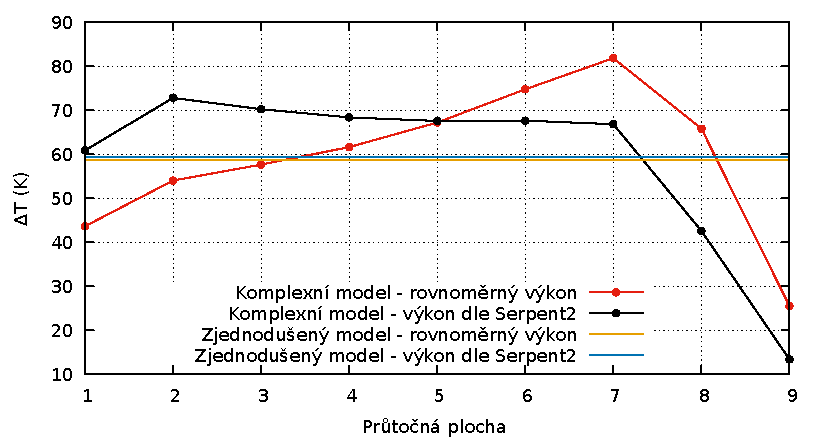
\includegraphics[width=\textwidth]{./04_TH_model_IRT/grafy/deltaT_irt4m_8_trubka.pdf}
	\caption{Ohřev na výstupu z jednotlivých kanálů pro jednotlivé modely.}
	\label{fig:ohrev_kanal}
\end{figure}
\begin{table}[H]
	\centering
	\caption{Ohřev chladiva na výstupu z PČ pro jednotlivé kanály (RV - rovnoměrný výkon, S - výkon dle Serpent2, KM \& JM - komplexní a zjednodušený model).}
	\label{tab:ohrev_irt_nat_conv}
	\begin{tabular}{llllllllll}
		\hline
		& \multicolumn{9}{c}{Trubka} \\ \hline
			$\Delta T_{out}$ (K) & 21 & 22 & 23 & 24 & 25 & 26 & 27 & 28 & 29          \\ \hline
		RV - KM   & 43,6     & 54,0    & 57,7    & 61,6    & 67,2    & 74,8    & 81,9    & 65,8    & 25,5    \\
		 S - KM     & 60,9    & 72,8    & 70,3    & 68,4    & 67,6    & 67,6    & 66,9    & 42,6    & 13,3     \\
		 RV - JM   & 58,7    &          &          &          &          &          &          &          &                         \\
		 S - JM & 59,3    &          &          &          &          &          &          &          &          \\         \hline      
	\end{tabular}
\end{table}

\begin{figure}[H]
	\centering
	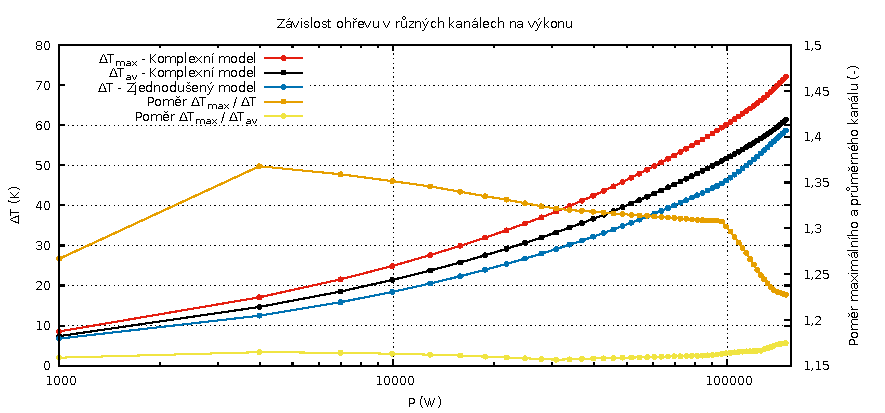
\includegraphics[width=\textwidth]{./04_TH_model_IRT/grafy/ohrev_rovn.pdf}
	\caption{Závislost ohřevu pro komplexní a zjednodušený model - rovnoměrný výkon (poměr teplot je poměr rozídlu teploty na výstupu z kanálu zjednodušeného modelu a komplexního modelu).}
	\label{fig:ohrev_vykon_rovn}
\end{figure}
\begin{figure}[H]
	\centering
	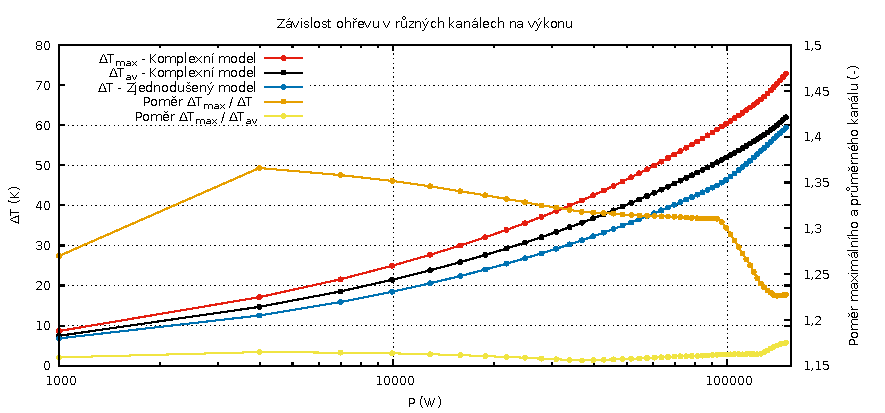
\includegraphics[width=\textwidth]{./04_TH_model_IRT/grafy/ohrev_serpent.pdf}
	\caption{Závislost ohřevu pro komplexní a zjednodušený model - výkon dle Serpent2 (poměr teplot je poměr rozídlu teploty na výstupu z kanálu zjednodušeného modelu a komplexního modelu).}
	\label{fig:ohrev_vykon_serpent}
\end{figure}

\subsection{Výskyt povrchového varu}
\label{subsec:nat_conv_var}
Možný výskyt varu v této sekci představuje stav, kdy teplota HS je vyšší než teplota sytosti kapaliny. Výkon jedné HS představující trubku PČ je \SI{1,875e4}{\watt}, tedy celkový výkon PČ je \SI{1,5e5}{\watt}.
Jak již bylo avizováno, tak při rozdělení výkonu dle programu Serpent je rozdělení teplot daleko rovnoměrnější, cž vede i k rovnoměrnějšímu výskytu možného povrchového bublinkového varu. Zároveň lze ale pozorovat, že konjukce trubek nemá na možný výskyt povrchového varu vliv.
\begin{figure}[H]
	\centering
	\begin{minipage}{.5\textwidth}
		\centering
		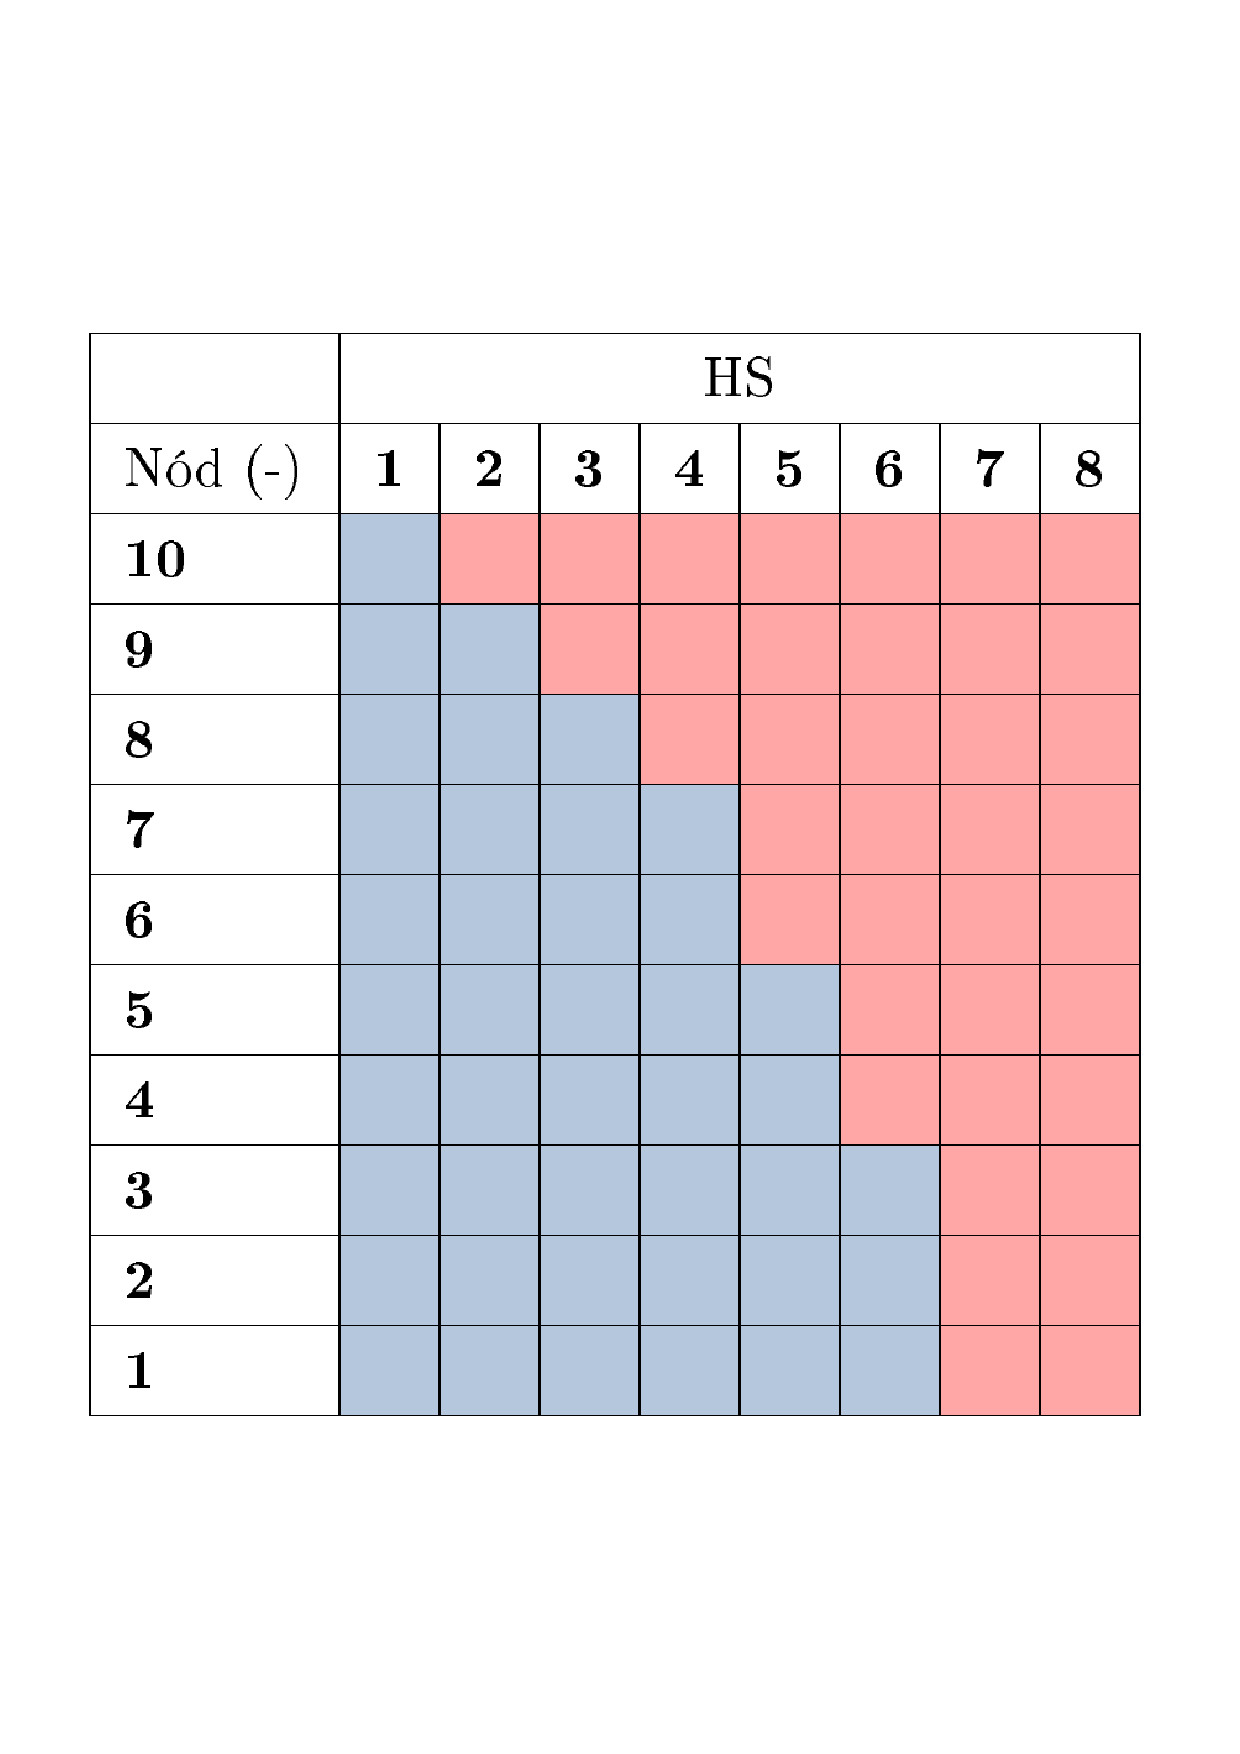
\includegraphics[width=0.98\textwidth, trim={1cm 5.5cm 0.5cm 5.5cm}, clip]{./04_TH_model_IRT/grafy/var_rovn_komplex.pdf}
		\caption{Komplexní model}
		\label{fig:var_komplex_rovn}
	\end{minipage}%
	\begin{minipage}{.5\textwidth}
		\centering
		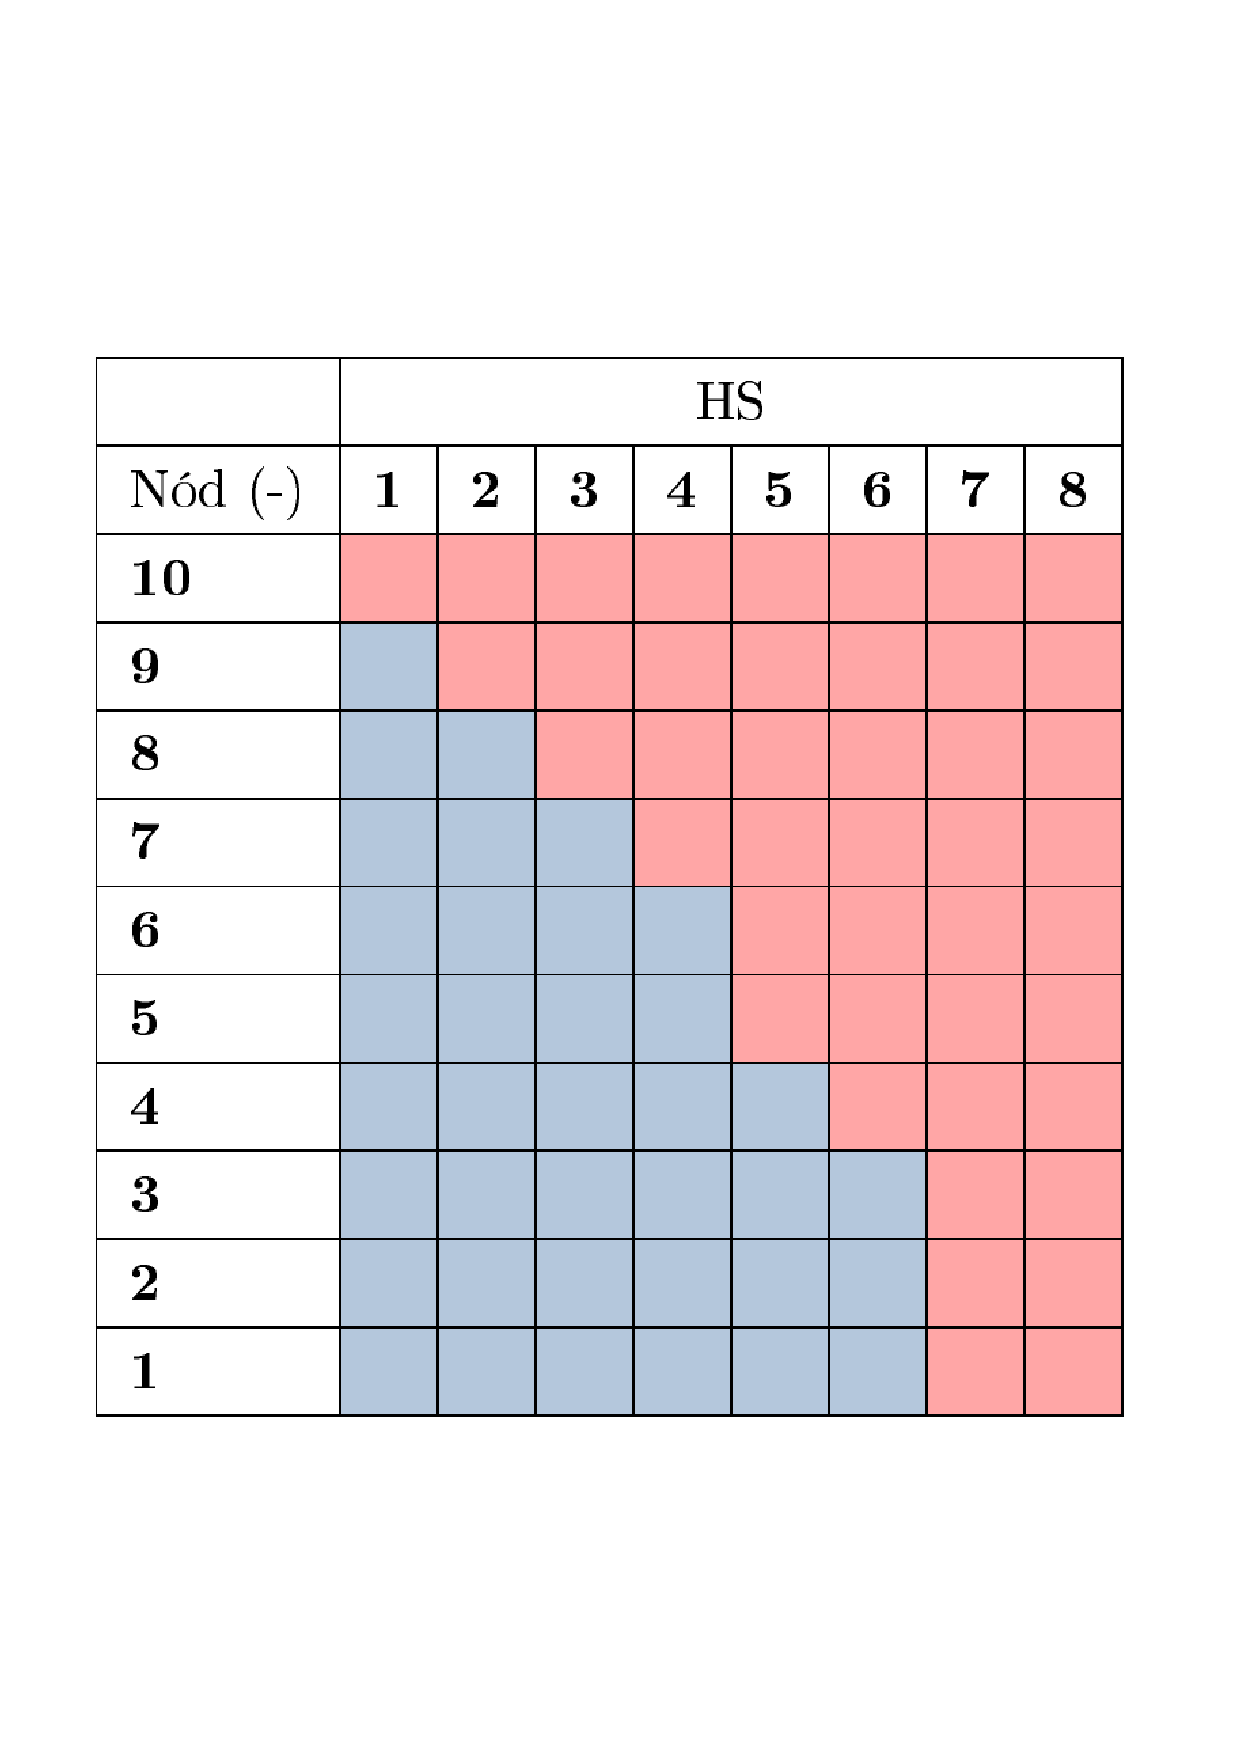
\includegraphics[width=\textwidth, trim={1cm 5.5cm 0.5cm 6cm}, clip]{./04_TH_model_IRT/grafy/var_rovn_jedno.pdf}
		\caption{Zjednodušený model}
		\label{fig:var_jedno_rovn}
	\end{minipage}
\caption{Možný výskyt povrchového bublinkového varu - rovnoměrné rozdělení výkonu (červeně nódy označují možný výskyt varu, modré přirozenou konvekci bez změny fáze).}
\label{fig:var_rovn}
\end{figure}
\begin{figure}[H]
	\centering
	\begin{minipage}{.5\textwidth}
		\centering
		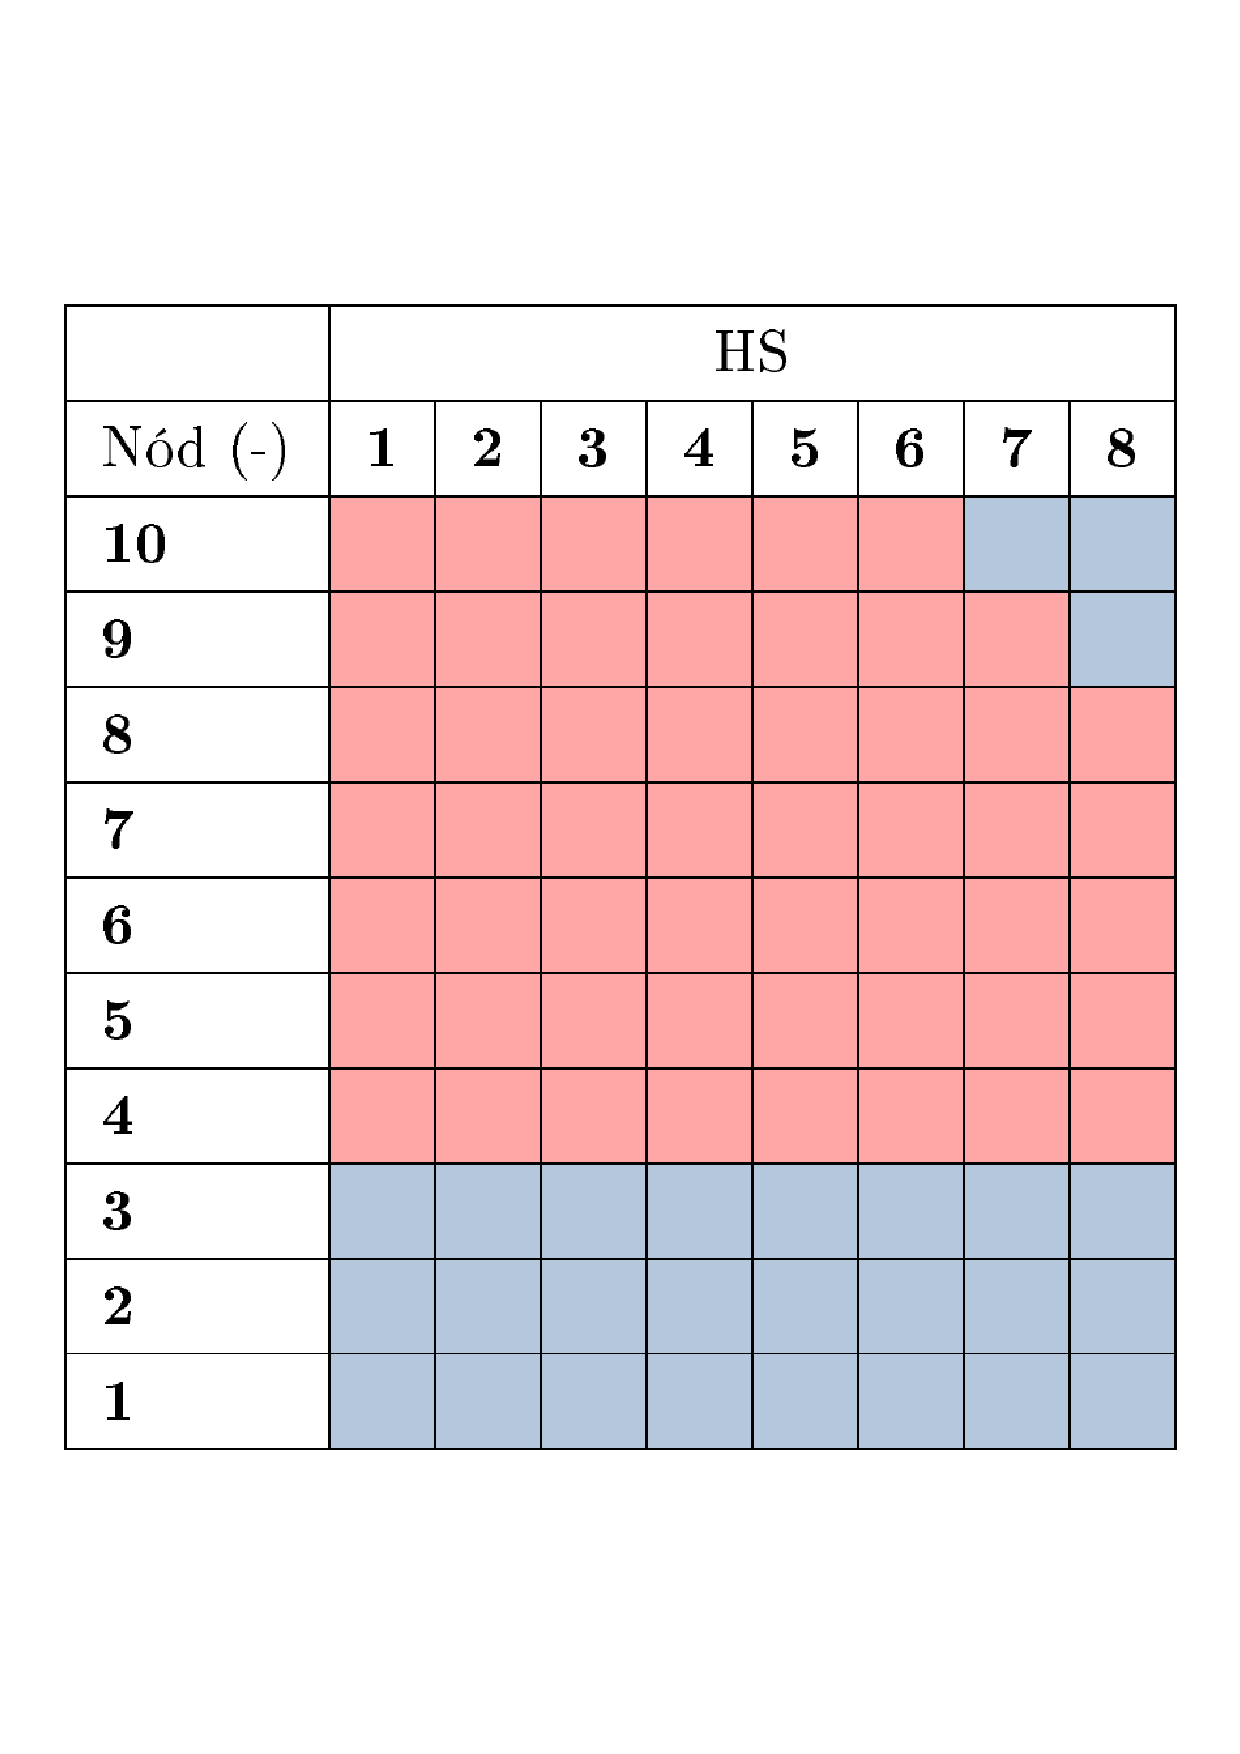
\includegraphics[width=0.98\textwidth, trim={0.5cm 4cm 0cm 5cm}, clip]{./04_TH_model_IRT/grafy/var_serpent_komplex.pdf}
		\caption{Komplexní model}
		\label{fig:var_komplex_serpent}
	\end{minipage}%
	\begin{minipage}{.5\textwidth}
		\centering
		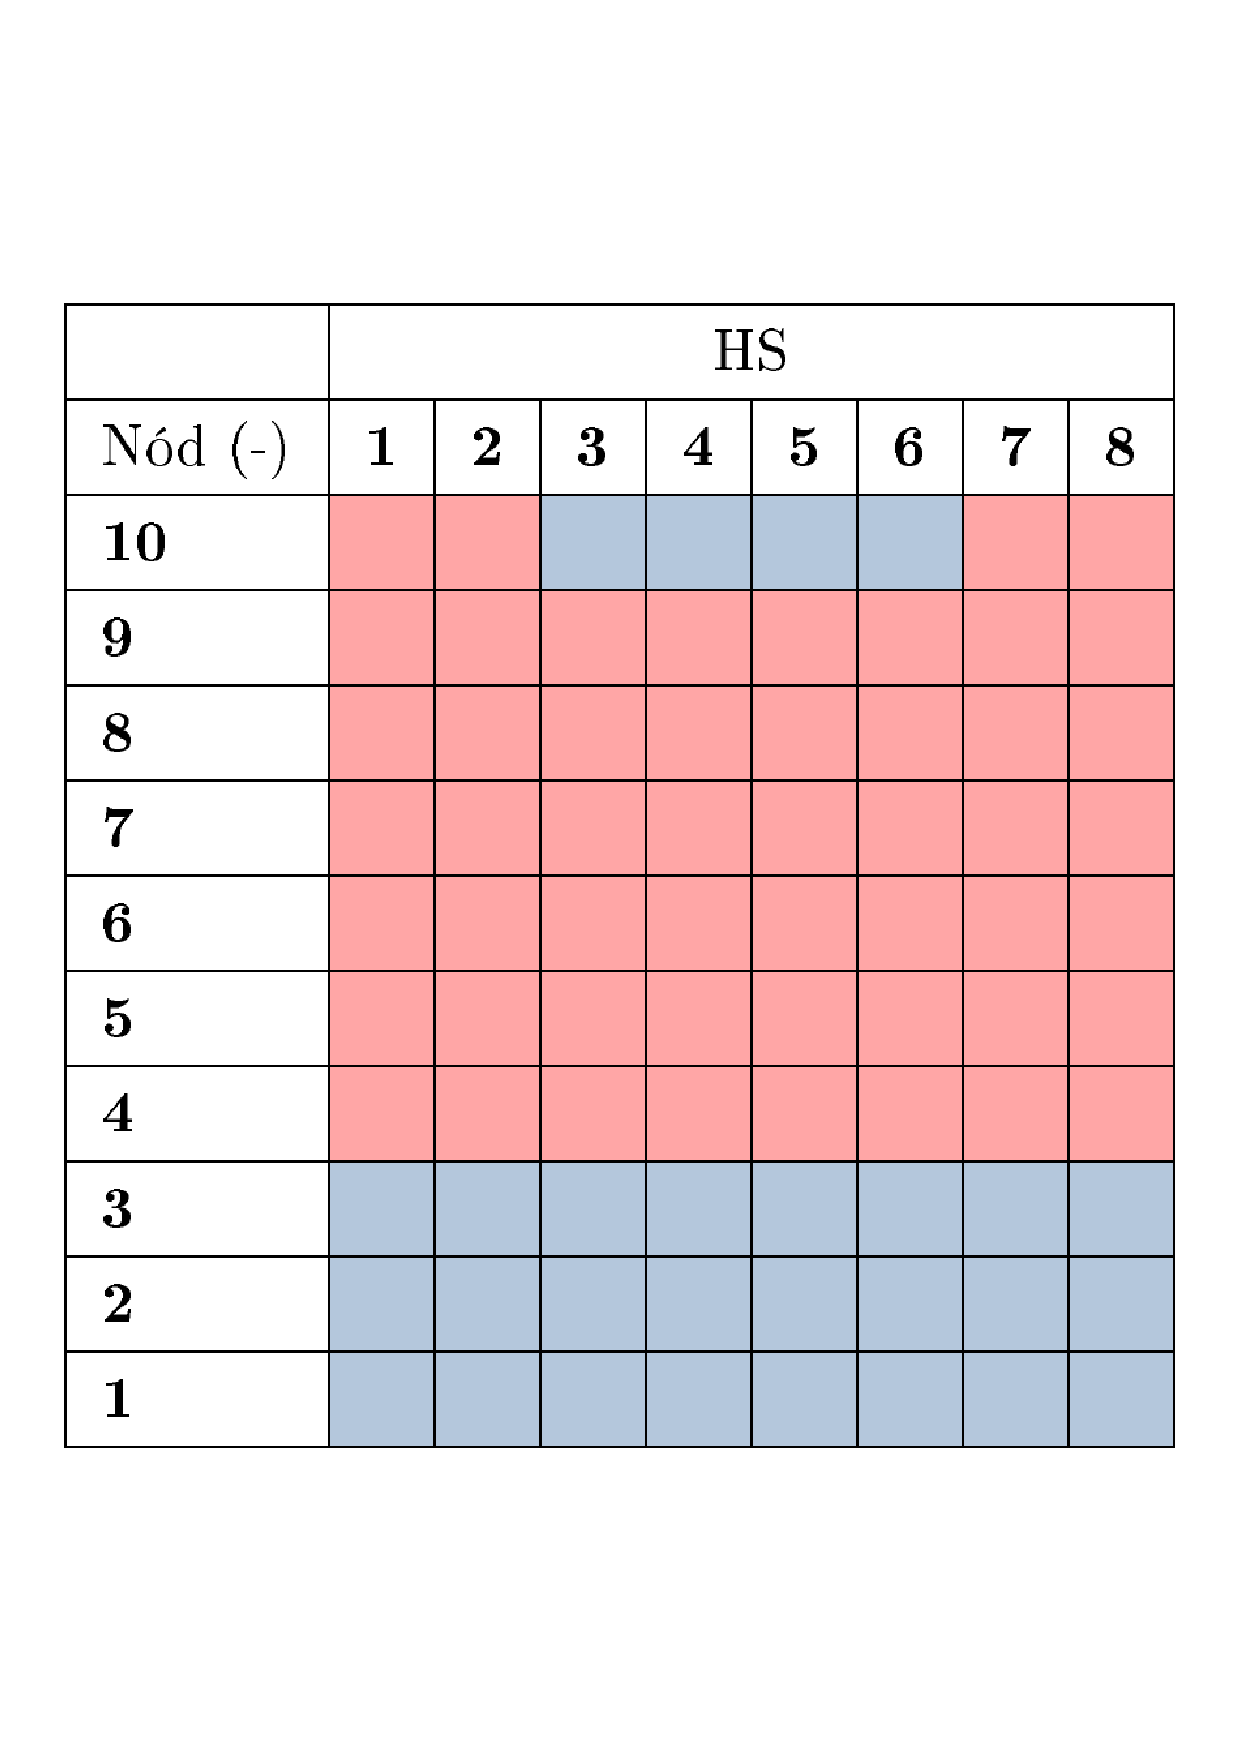
\includegraphics[width=0.98\textwidth, trim={0.5cm 4cm 0cm 5cm}, clip]{./04_TH_model_IRT/grafy/var_serpent_jedno.pdf}
		\caption{Zjednodušený model}
		\label{fig:var_jedno_serpent}
	\end{minipage}
	\caption{Možný výskyt povrchového bublinkového varu - rozdělení výkonu dle Serpent2 (červeně nódy označují možný výskyt varu, modré přirozenou konvekci bez změny fáze).}
	\label{fig:var_serpent}
\end{figure}
\subsection{Zhodnocení sjednocení průtočných kanálů}
\label{subsec:nat_conv_zaver}
Sjednocení průtočných kanálů nenaznačují žádný velký problém pro další použití. Největším problémem je právě ztráta informace o maximálním ohřevu, což může být do jisté kompenzováno již zmiňovaným \uv{faktorem ohřevu}. Ukazuje se, že tento faktor zůstává konstantní pro široké rozmezí výkonů a je možné tedy provést odhad maximální teploty na výstupu z PČ. Dále se ukazuje, že rozložení výkonu způsobuje rovnoměrnější ohřev a možný výskyt povrchového bublinkového varu. Sjednocení na možný povrchový var nemá velký vliv. Největším problémem pro bezpečnostní analýzy by v tomto případě byla situace, kdy by v maximálním kanálu docházelo k objemovému varu. Vznik objemového varu ovšem není součástí základních projektových podmínek ani rozšířených projektových podmínek \cite{fejt, rataj_bezpecnosti_zprava_VR_1}.



\section{Sjednocení topných komponent} \label{sec:sjednoceni_topnych_komponent}
Pro analýzu přirozeného proudění skrz PČ IRT-4M dává smysl využít počet HS odpovídající počtu palivových trubek, tedy 8 topných jednotek. Pro analýzu celé aktivní zóny reaktoru VR-1 by bylo třeba vložit okolo 8$\times$16 HS, což by mohlo být problematické. Proto dává smysl vytvořit zjednodušený model se sjednocenými topnými komponentami. Při přechodu na jednu zjednodušenou HS je třeba zachovat stejnou teplosměnnou plochu a hydraulický průměr. V tab. \ref{tab:jednotkovy_model} geometrie této HS uvedena. Vnější průměr sjednocené HS v tomto případě převyšuje vnější rozměr palivové trubky 1 viz tab. \ref{tab:prilohy_irt_geometrie}, což je konstruktem požadavku na zachování teplosměnné plochy a hydraulického průměru. Tato HS chováním reprezentuje komplexní sadu 8 HS a je dále využitá jakožto zdroj tepla pro PČ v termohydraulickém modelu VR-1. Zjednodušený model PČ s sjednocenou HS bude dále označován jako \uv{jednotkový model}. Rozdíl zjednodušeného a jednotkového modelu je pouze v HS, geometrie trubek a obtoku zůstává stejná. Axiální rozložení výkonu odpovídá tab. \ref{tab:rozlozeni_vykonu_irt_serpent} uvedené v předchozí sekci.
\begin{table}[H]
	\centering
	\caption{Geometrie sjednocené HS.}
	\label{tab:jednotkovy_model}
	\begin{tabular}{cc}
		\hline
		$ r_o $ (mm) & 210,11  \\
		$ r_i $ (mm) & 207,82  \\
		$ h $ (mm) 	 & 588 \\
		
		\hline
	\end{tabular}
\end{table}
\subsection{Výpočet a zhodnocení sjednocení HS}
Analogicky k předchozí části jsou v tab. \ref{tab:sjednoceni_hs} uvedeny parametry pro zjednodušený model (1 průtočná trubka a 8 HS) a jednotkový model (1 průtočná trubka a 1 sjednocená HS). Namísto možného výskytu povrchového varu je v tabulce uvedena maximální teplota HS.
\begin{table}[H]
	\centering
	\caption{Celkový průtok, ohřev a maximální teplota HS pro zjednodušený a jednotkový model.}
	\label{tab:sjednoceni_hs}
	\begin{tabular}{cccc}
		\hline
		& \multicolumn{2}{l}{TH model}          &                    \\
		& zjednodušený (serpent) & jednotkový   & rel. odch. (\%)    \\
		\hline \hline

		$G$ (m$^3$/h) & 2,261 & 2,258 & 0,11\\
		$\Delta T$ (K)                & 59,31                  & 59,38        & 0,12 \\
		$T_{\text{HS},\text{max}}$ (K)             & 384,85                 & 383,54       & 0,34\\
		\hline
	\end{tabular}
\end{table}
 Změna v průtoku chladiva skrz PČ a změna ohřevu je zanedbatelná, maximální teplota HS se liší o méně než 0,5 \%. Z uvedených výsledků vyplývá, že je možné považovat jednotkový model za způsobilý dalším výpočtům. Oproti zjednodušenému modelu je výhodou redukovaný počet HS, který by při složitějších výpočtech AZ mohl být komplikovaný.
\chapter{Termohydraulický model reaktoru VR-1}

\label{chap:th_model_vr_1}
%\section{Motivace}
%\label{sec:the_model_vr_1_motivace}
Studium přirozené konvekce na školním reaktoru VR-1 je klíčové pro zajištění bezpečného provozu tohoto zařízení. Při studiu nucené konvekce je průtok sledovaným objemem určen jako vstupní parametr, resp. jako okrajová podmínka. Pro přirozenou konvekci není průtok vstupním parametrem, ale je odvozen z teplotního gradientu a je dáno modelem samotného reaktoru. U výzkumných reaktorů bazénového typu (např. VR-1, TRIGA Mark II) musí být model reaktoru rozšířen o reaktorovou nádobu, aby bylo možné odhadnout celkový průtok skrze zónu \cite{TRIGA_CFD}. Cílem této kapitoly je popis termohydraulického modelu školního reaktoru VR-1 a studium vlivu nodalizace obtoku na přirozené proudění.

Na obr. \ref{fig:cfd_triga_reynolds} je pomocí CFD kódu uvedena Reynoldsova mapa, resp. rychlostní pole v případě přirozeného proudění skrze AZ reaktoru TRIGA Mark II (geometrie reaktoru TRIGA je zobrazena v příloze na obr. \ref{fig:triga_geometrie}). Reaktor TRIGA Mark II a školní reaktor VR-1 mají obdobnou konstrukci a oba jsou bazénového typu (viz obrázek \ref{fig:vr_1_geometrie} v příloze). Z obrázků \ref{fig:cfd_triga_reynolds} a \ref{fig:cfd_triga_velocities} vyplývá, že nejvíce turbulentní proudění nastává v prostoru nad aktivní zónou, tedy i v horní části vertikálního obtoku skrz reaktorovou nádobu. Obrázek \ref{fig:cfd_triga_velocities} naznačuje, že změna teplotního gradientu nad aktivní zónou vede k vzniku inverze proudění a tvorbě smyček. Z tohoto důvodu se tato kapitola soustředí především na studium této oblasti (viz obrázek \ref{fig:nod_00}). Dále je oblast volného objemu nad aktivní zónou označena jako "horizontální obtok" a komponenta 44 jako "vertikální obtok".



\begin{figure}[H]
	\centering
	\begin{subfigure}{0.5\textwidth}
		\centering
		\vspace{0cm}
		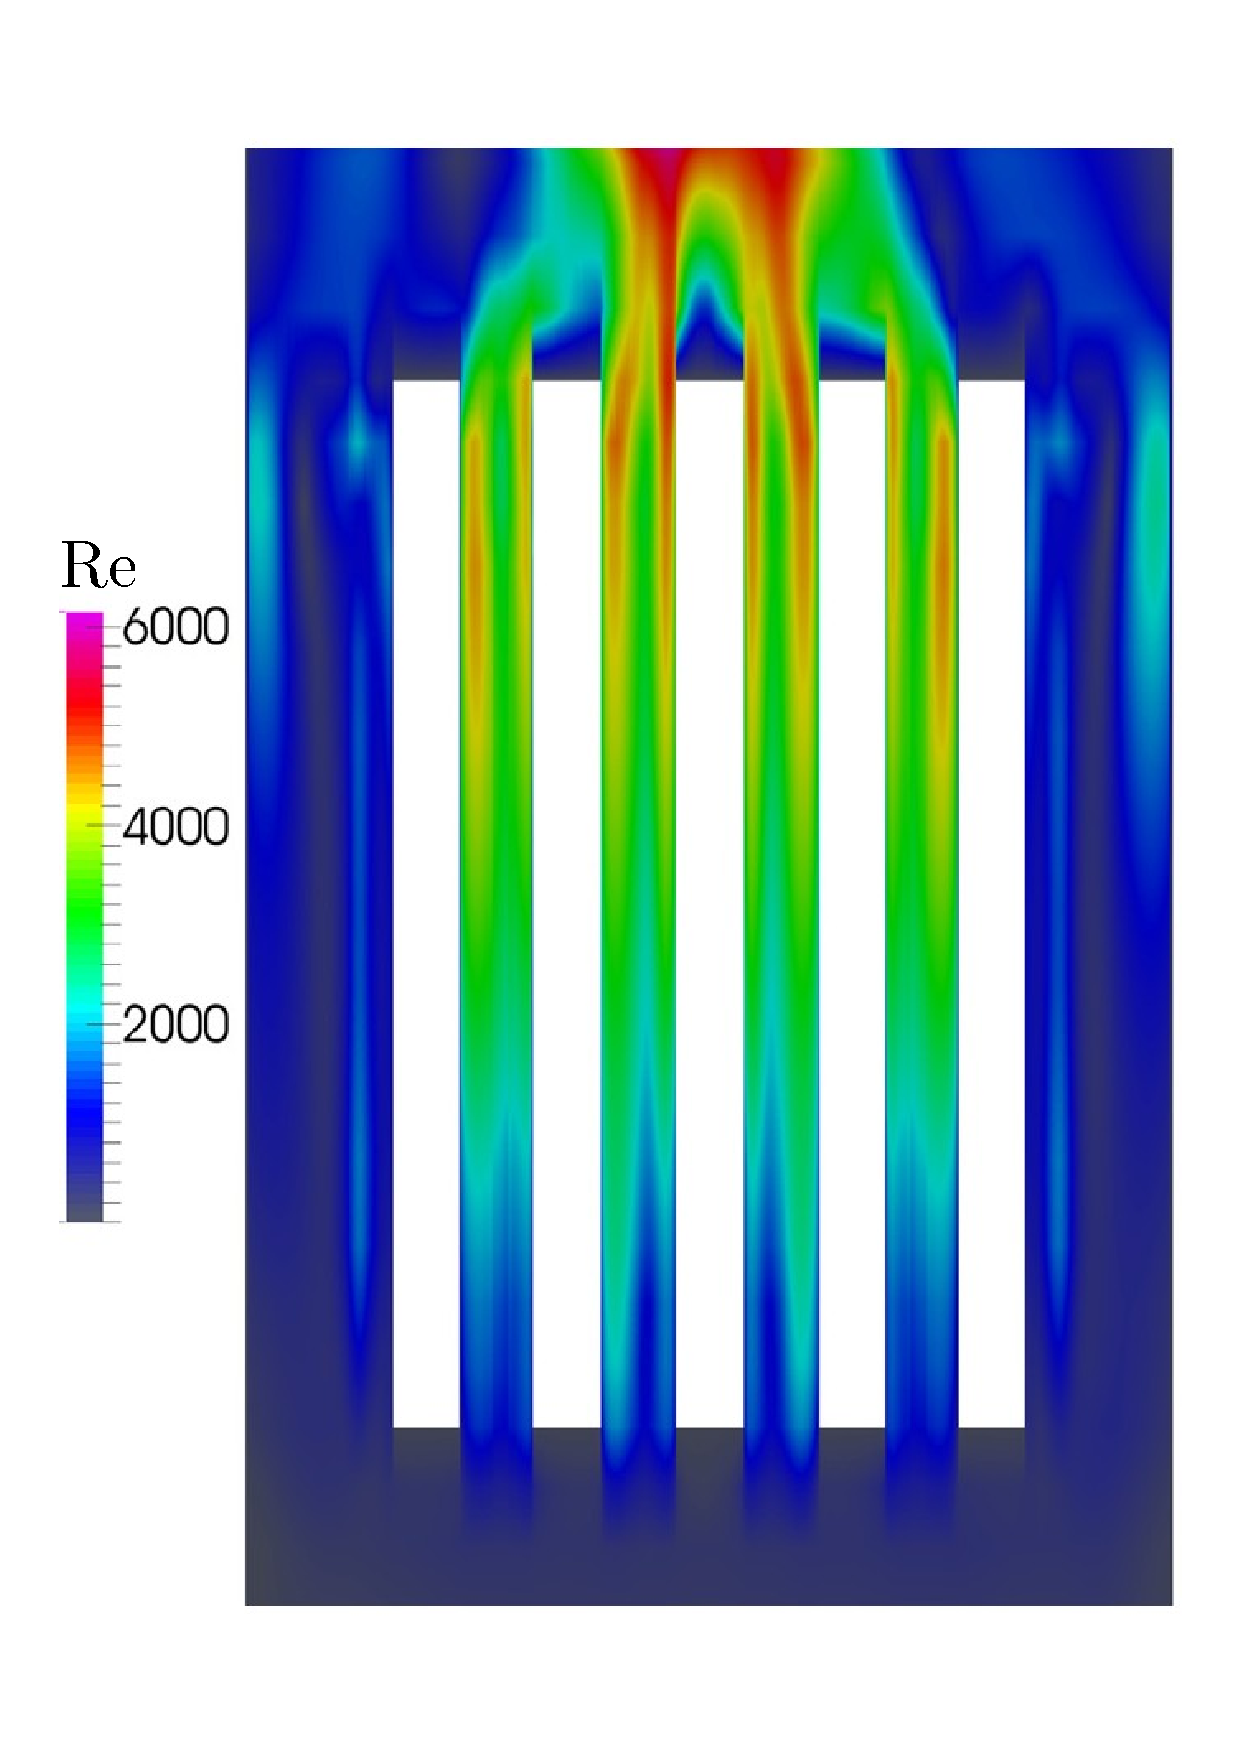
\includegraphics[width=0.6\textwidth, trim={1cm 2cm 1cm 2cm}, clip]{./05_TH_model_VR_1/obrazky/cfd_triga_reynolds_number.pdf}
		\vspace{0pt}
			\caption{Reynoldsova mapa}
			\label{fig:cfd_triga_reynolds}
	\end{subfigure}%
	\hfill
	\begin{subfigure}{0.5\textwidth}
		\centering
		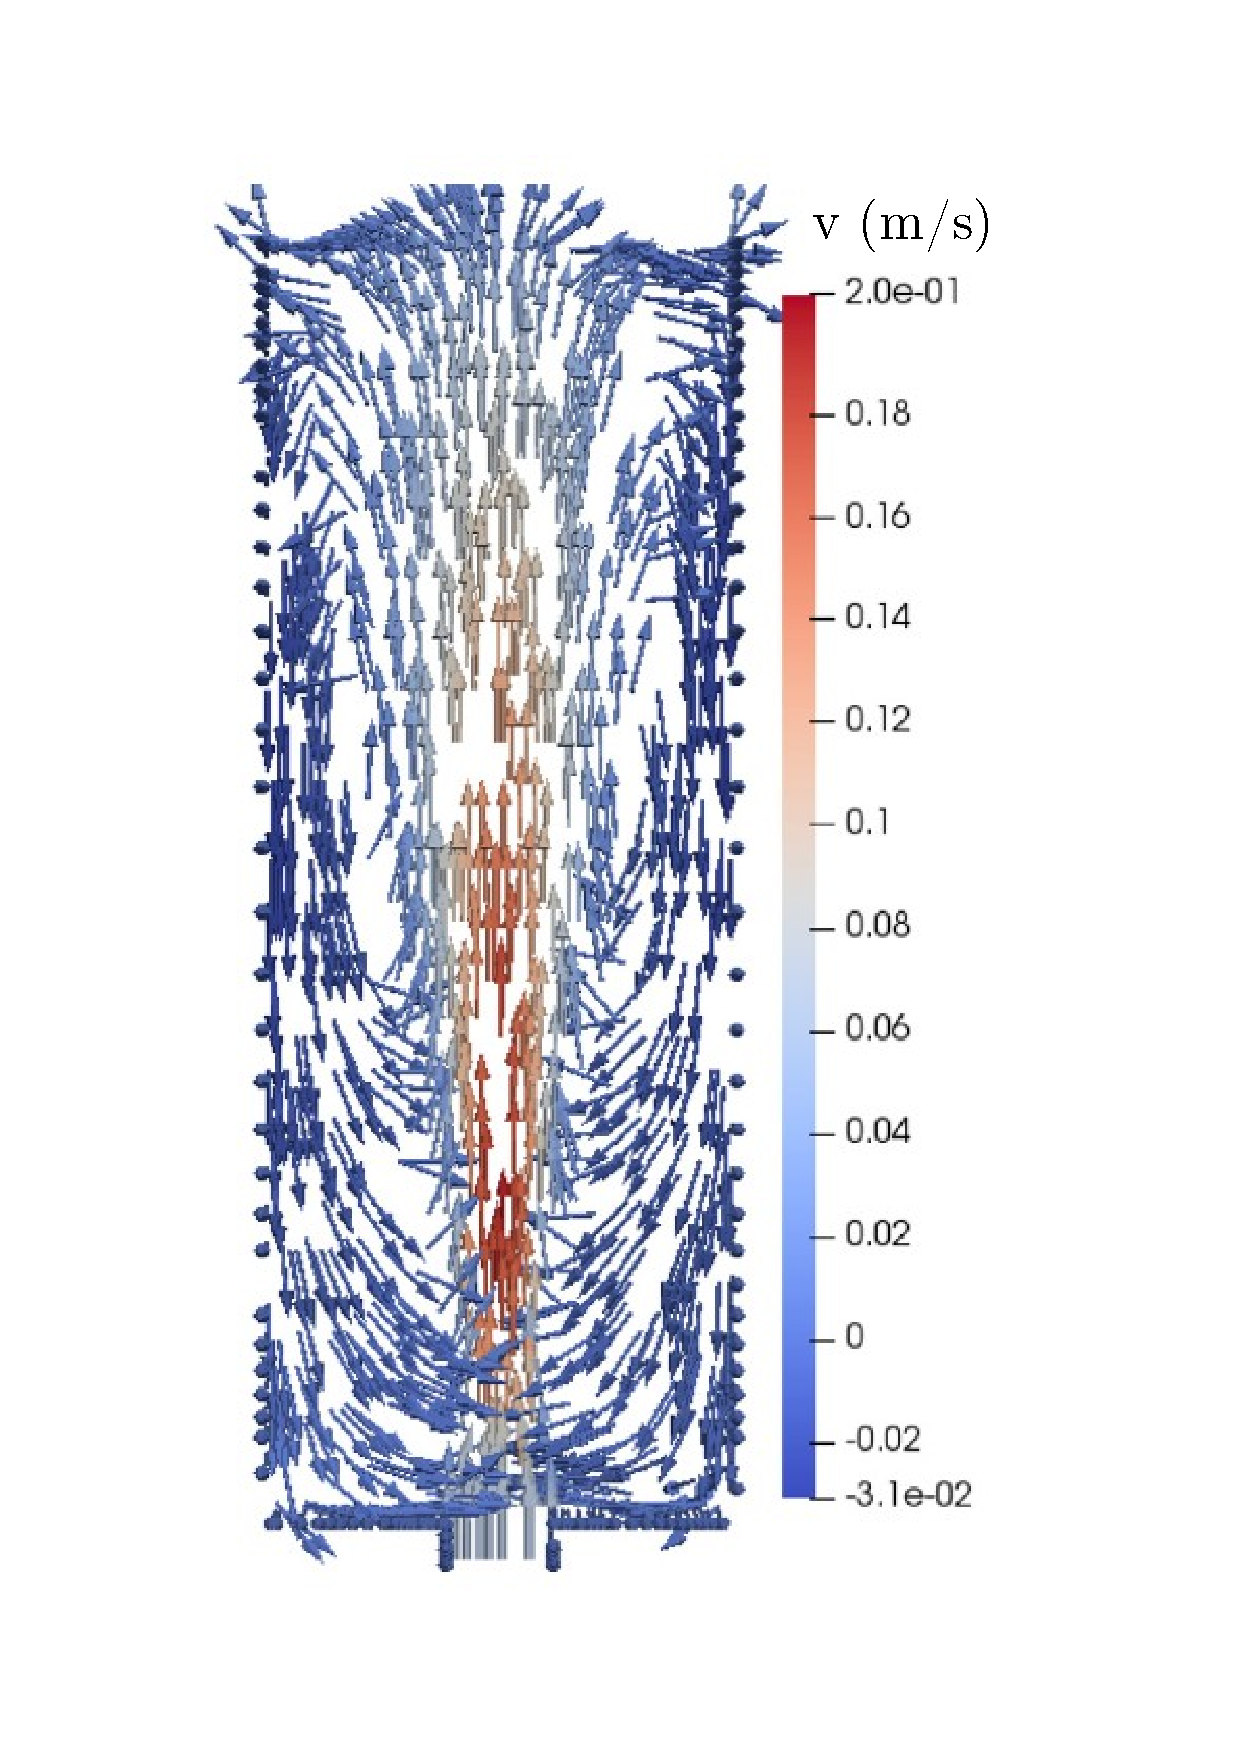
\includegraphics[width=0.6\textwidth, trim={2cm, 3cm, 2cm, 3cm}, clip]{./05_TH_model_VR_1/obrazky/triga_cfd_velocities.pdf}
		\caption{Rychlostní pole}
		\label{fig:cfd_triga_velocities}
	\end{subfigure}
	\caption{CFD výpočet přirozeného proudění skrze reaktor TRIGA MARK II \cite{TRIGA_CFD}.}
\end{figure}


\section{Referenční model}
\label{sec:referencni_model}
V této práci \cite{fejt} byl při tvorbě modelu školního reaktoru VR-1 opuštěn koncept dvoukanálového uspořádání, který využíval "průměrný" a "maximální" kanál pro reprezentaci aktivní zóny reaktoru. Místo toho byla aktivní zóna sestavena z 16 palivových článků (PČ), z nichž každý byl reprezentován jednotkovým modelem (viz sekce \ref{sec:sjednoceni_topnych_komponent}). Kvůli omezenému počtu připojitelných komponent k jednotce BRANCH (komponenta 100 a 102) byla aktivní zóna reprezentována dvěma skupinami po osmi PČ, které byly propojeny spojovací jednotkou. Všechny jednotkové modely vychází z modelu 8-trubkového PČ bez vytěsnitele, přičemž axiální rozložení výkonu jednotlivých PČ odpovídá tabulce \ref{tab:rozlozeni_vykonu_irt_serpent}. Geometrie trubek horizontálního a vertikálního obtoku je stejná jako v modelu, který je popsán na obrázcích \ref{fig:irt_nat_conv_komplex} a \ref{fig:irt_nat_conv_jedno}. Zapojení komponent 40-48 vychází z práce \cite{fejt}. Model na obrázku \ref{fig:nod_00} je označen jako "referenční", resp. jako model NOD00. Nodalizace reaktoru bude podrobněji rozebrána v následujících kapitolách.

V případě referenčního modelu je horizontální obtok napojen až v posledním nódu trubky 40. Voda je vytlačena z AZ až na úroveň hladiny, kde se odpojuje do horizontálního obtoku. V tomto uspořádání je teplotní gradient mezi výstupem z AZ reaktoru a TDV 50 představující volnou hladinu největší (tlak \SI{1,5e5}{\pascal} Pa a teplota vody 297 K). Nikde v trubce 40 nedochází k ochlazení bočním vtokem. U referenčního modelu je proto očekáván nejvyšší průtok.

Výkon školního reaktoru VR-1 je pro studium přirozeného proudění příliš nízký (\SI{1e2}{\watt}, nárazově \SI{5e2}{\watt}). Proto je v následujícím textu uvažován výkon jednoho PČ \SI{1e4}{W} (celkový výkon AZ \SI{1,6e5}{\watt}), při kterém je studium přirozené konvekce názornější. Stále se jedná o jednofázové proudění podchlazené kapaliny. Průběh výkonu jednotkového modelu PČ je uveden v příloze v Tab. \ref{tab:vykon_model} (více o jednotkovém modelu v sekci \ref{sec:sjednoceni_topnych_komponent}). Aktivní zóna je tvořena 16 PČ, každý článek má výkon \SI{10e4}{\watt}. Celkový výkon reaktoru dosahuje v čase 20 s \SI{1,6e5}{\watt}. Na obr. \ref{fig:temp_fuel_nod00} je uvedeno rozdělení teplot chladiva v PČ v čase 10 s, 20 s, 30 s a 40 s po dosažení výkonu \SI{10e4}{\watt}. Celkový průtok PČ je uveden na obr. \ref{fig:nod_00_mass_flow_rate}.
\subsection{Výsledky}

 
\begin{figure}
	\centering
	\includegraphics[width=\textwidth, trim={1cm 218cm 148cm 5cm}, clip]{./06_hodnoceni_TH_modelu/obrazky/nod_00_recirculation.pdf}
	\caption{Termohydraulický model reaktoru VR-1.}
	\label{fig:nod_00}
\end{figure}


\begin{figure}[H]
	\centering
	\begin{subfigure}{0.5\textwidth}
		\centering
		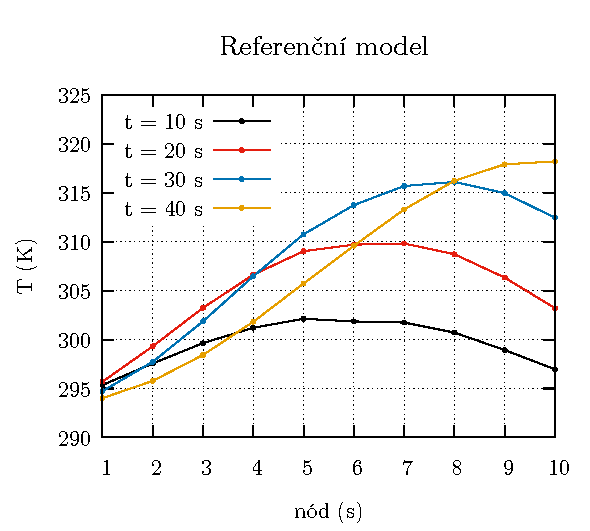
\includegraphics[width=\textwidth, trim={0cm 0cm 0cm 0cm}, clip]{./05_TH_model_VR_1/grafy/nod_00_temp_distribution_fuel.pdf}
		\caption{Axiální rozložení teplot vody v PČ.}
		\label{fig:temp_fuel_nod00}
	\end{subfigure}%
	\hfill
	\begin{subfigure}{0.5\textwidth}
		\centering
		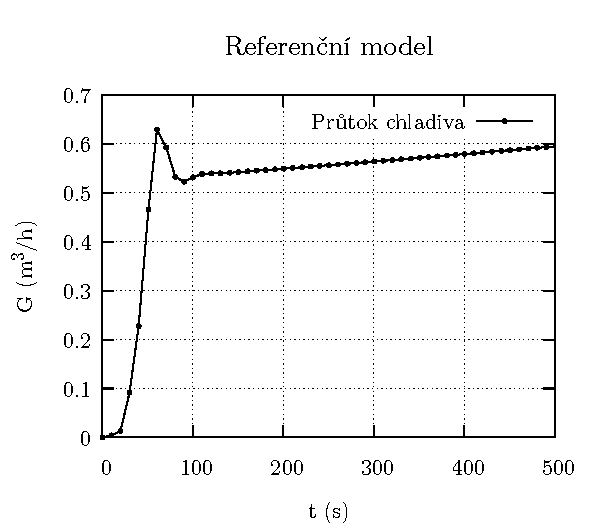
\includegraphics[width=\textwidth, trim={0cm 0cm 0cm 0cm}, clip]{./05_TH_model_VR_1/grafy/nod_00_mass_flow_rate_fuel.pdf}
		\caption{Celkový průtok skrze PČ.}
		\label{fig:nod_00_mass_flow_rate}
	\end{subfigure}
	\caption{Popis přirozeného proudění skrze palivový článek pro referenční model.}
\end{figure}
Na obr. \ref{fig:temp_fuel_nod00} a \ref{fig:nod_00_mass_flow_rate} lze pozorovat vznik přirozeného proudění chladiva v palivovém článku (PČ) v závislosti na čase a výkonu. Po dosažení výkonu $10^4$ W v čase 10 s je rozložení teplot symetrické, což odpovídá symetrii výkonu po axiální ose. V dalších časových krocích se teplotní maximum posouvá zhruba o 1 nód za 10 s v důsledku vzniku přirozené konvekce. Proudění ohřívaného objemu vede ke snížení teploty v dolní části palivového článku vlivem promíchávání se vstupujícím chladivem.

Na stejném obrázku je také vykreslen časový průběh průtoku chladiva skrze PČ. Vliv časového zpoždění je zde také pozorovatelný. V čase 0-60 s dochází k nárůstu průtoku v důsledku ohřevu chladiva v AZ reaktoru. Vyšší průtok v tomto případě způsobuje lepší přestup tepla a tedy i nižší teplotní gradient mezi AZ a vstupem do horizontálního obtoku, což vede ke snížení průtoku až do času 90 s. Následně se průtok ustálí okolo 100 s a hodnota průtoku lineárně roste. Důvodem je absence teplotních ztrát v modelu.

Na obrázku \ref{fig:nod_00_temp_pipe_40} jsou zobrazeny teploty v trubce 40 pro jednotlivé nódy. Teplota v nódu 1 se po 800 s ustálí, přičemž dochází k postupnému ohřevu výše položených nódů. Jelikož model neuvažuje tepelné ztráty, tak není jisté jak by vypadalo rozložení teplot době delší než 1200 s. Fyzikální význam by byl diskutabilní. Podrobnější rozložení teplot je popsáno v příloze na obrázcích \ref{fig:temp_dist_srovnani_prilohy_100s} až \ref{fig:temp_dist_srovnani_prilohy_600s}.




 
 \begin{figure}[H]
 	\centering
 	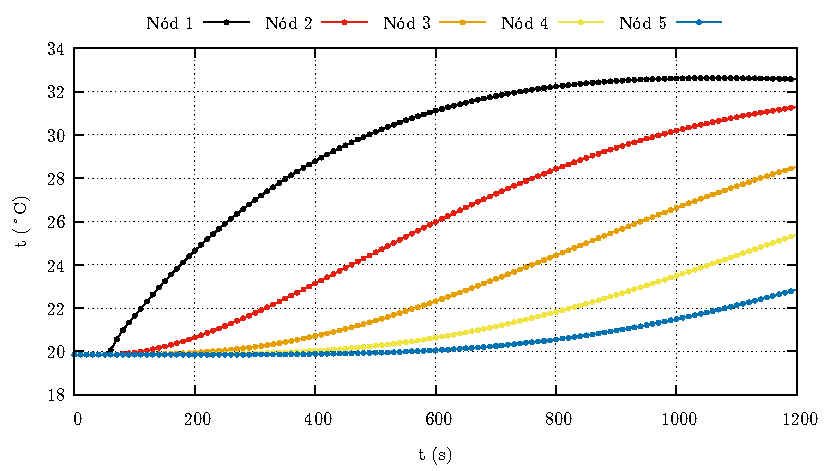
\includegraphics[width=0.8\textwidth]{./05_TH_model_VR_1/grafy/t_nod_00.pdf}
 	\caption{Časový vývoj teplot v jednotlivých nódech trubky 40.}
 	\label{fig:nod_00_temp_pipe_40}
 \end{figure}
 \section{Model NOD01}
 \label{sec:nod_01}
V referenčním modelu reaktoru VR-1 v programu RELAP5 je při simulaci přirozeného proudění předpokládána absence recirkulace ve volném objemu nad AZ, neboť je v tomto případě ohřátá voda nucena proudit až na úroveň vodní hladiny, kde se dochází k vstupu do horizontálního obtoku z posledního nódu trubky 40. Ve skutečnosti však může při přirozeném proudění docházet k odpojení vody v libovolné výšce objemu vytyčeného nad aktivní zónou. Z tohoto důvodu je trubka 42 nahrazena pěti horizontálními trubkami (trubka 170-174) viz obr. \ref{fig:nod_01}, přičemž celkový objem těchto trubek je zachován. Kompletní model je prezentován na obr. \ref{fig:nod_01_prilohy} v příloze.

  
 \begin{figure}[H]
 	\centering
 	\includegraphics[width=0.8\textwidth,  trim={7.5cm 243cm 155cm 5cm}, clip]{./07_prilohy/recirkulace/nod_01_recirculation.pdf}
 	\caption{Nodalizace horizontálního obtoku - model NOD01}
 	\label{fig:nod_01}
 \end{figure}
\subsection{Výsledky}
Z předchozího textu vyplývá, že hlavními sledovanými parametry pro srovnání referenčního a renodalizovaného modelu jsou celkový průtok skrze aktivní zónu, průtok skrze jednotlivé trubky horizontálního obtoku a rozložení teplot chladiva v trubce 40.

Renodalizovaný model NOD01 prokazuje identické chování jako referenční model v intervalu 0-200 s. Po ustálení průtoku je hodnota G(t) pro model NOD01 v čase konstantní, zatímco v referenčním modelu roste s konstantní rychlostí. Při pozorování horizontálního obtoku se ukazuje, že na rozdíl od referenčního modelu dochází k inverzi proudění v trubkách 170 a 171. Ohřáté chladivo teče vzhůru a v horizontálním kladném směru proudí trubkou 172, 173 a 174 do trubky 175, kde dochází k promíchávání. Část chladiva se následně vrací trubkou 170 a 171, kde v trubce 40 ochlazuje chladivo vystupující z AZ. Situace je ilustrována na Obr. \ref{fig:nod_01}.

Toto promíchání chladiva s ochlazenou kapalinou vstupující z trubek 170 a 171 má vliv na rozložení teplot v objemu trubky 40 viz příloha obr. \ref{fig:temp_dist_srovnani_prilohy_100s} až \ref{fig:temp_dist_srovnani_prilohy_600s}. Renodalizovaný model NOD01 tak více odpovídá reálné situaci. Je třeba zmínit, že model NOD01 neobsahuje tepelné ztráty, což má za následek konstantní nárůst teploty. Otázkou zůstává, do jaké míry je možné tento ohřev považovat za reprezentativní. 




 \begin{figure}[H]
 	\centering
 	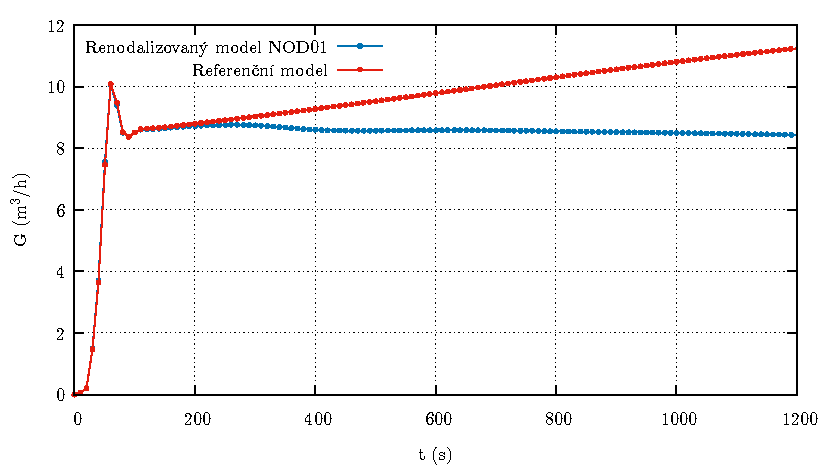
\includegraphics[width=0.8\textwidth]{./05_TH_model_VR_1/grafy/nod_01_mass_flow_rate_vertical.pdf}
 	\caption{Průtok skrze AZ reaktoru VR-1 - referenční a renodalizovaný model NOD01. }
 	\label{fig:nod_01_mass_flow_rate_vertical}
 \end{figure}
\begin{figure}[H]
	\centering
	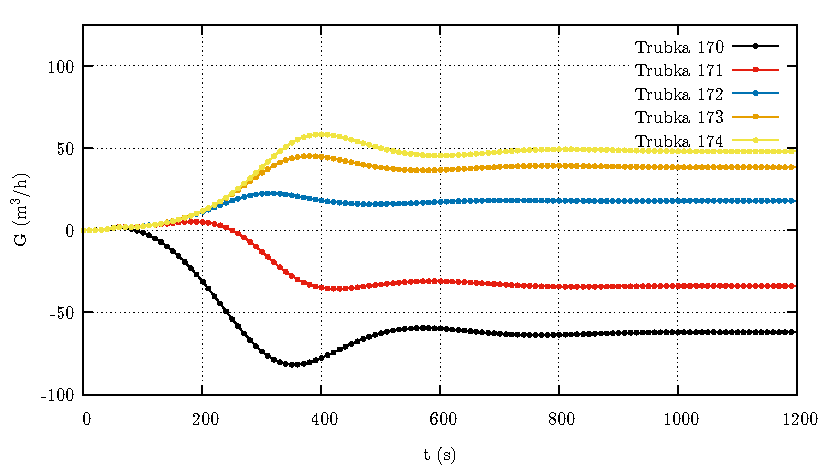
\includegraphics[width=0.8\textwidth]{./05_TH_model_VR_1/grafy/nod_01_mass_flow_rate_horizontal.pdf}
	\caption{Průtok skrze trubky 170 - 174 (viz obr. \ref{fig:nod_01}) - renodalizovaný model NOD01.}
	\label{fig:nod_01_mass_flow_rate_horizontal}
\end{figure}
\begin{figure}[H]
	\centering
	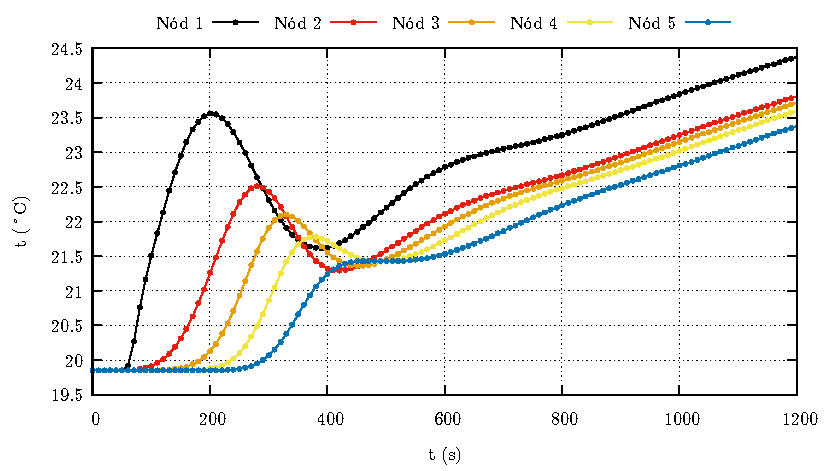
\includegraphics[width=0.8\textwidth]{./05_TH_model_VR_1/grafy/t_nod_01.pdf}
	\caption{Teplotní vývoj v trubce 40 - model NOD01.}
	\label{fig:nod_01_temp_pipe_40}
\end{figure}
%\begin{figure}[H]
%	\centering
%	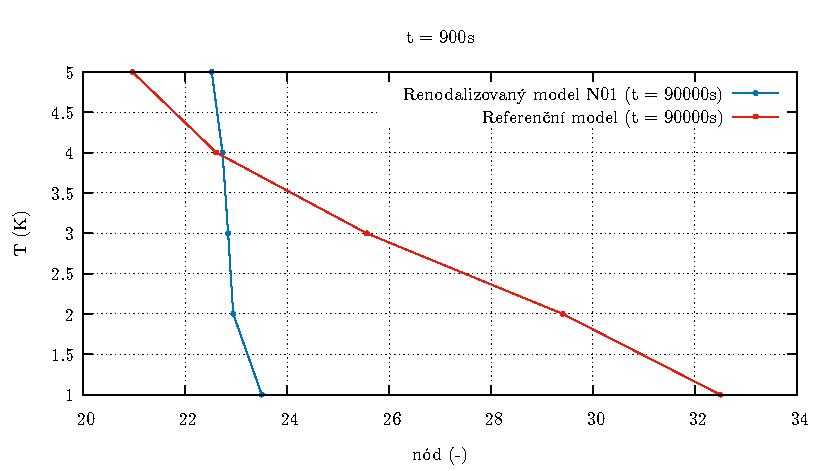
\includegraphics[width=0.8\textwidth]{./05_TH_model_VR_1/grafy/nod_01_900.pdf}
%	\caption{Distribuce teplot v trubce 40 v čase 900 s.}
%	\label{fig:nod_01_temp_distribution}
%\end{figure}
 \section{Model NOD02}
 \label{sec:nod_02}
 Druhý renodalizovaný model s označením NOD02 je konstruován za účelem studia vlivu nodalizace vertikálního obtoku. Konstrukce vertikálního obtoku i s výslednými směry proudění je ilustrována na obrázku \ref{fig:nod_02} a kompletní schéma modelu je uvedeno na obr. \ref{fig:nod_02_prilohy} v příloze. Vertikální obtok je sestaven symetricky, přičemž celkový objem trubek a kontrolních objemů je zachován. Trubka 44 v referenčním modelu je nahrazena párem propojených trubek s označením 169 a 171, které umožňují vzniku příčného proudění a redistribuci průtoku ve vertikálním směru v obou trubkách.
 \begin{figure}[h]
 	\centering
 	\includegraphics[width=0.6\textwidth,  trim={18cm 225cm 152cm 10cm}, clip]{./07_prilohy/recirkulace/nod_02_recirculation.pdf}
 	\caption{Nodalizace vertikálního obtoku - model NOD02}
 	\label{fig:nod_02}
 \end{figure}
\subsection{Výsledky}
Průtok skrze aktivní zónu reaktoru je v případě modelu NOD02 totožný s referenčním viz obr. \ref{fig:nod_02_mass_flow_rate_vertical}. Teplota v kontrolním objemu 167 je 293 K (teplota okrajové podmínky stanovené TDV 50 viz příloha obr. \ref{fig:nod_02_prilohy}). Je možné dále očekávat rozdílný průtok v obou směrech skrze SJ 178 až 185, a to z důvodu asymetrickému propojení s horizontálním obtokem. Průtok ve vertikálním obtoku je ilustrován na obrázcích \ref{fig:nod_02_mass_flow_rate_horizontal} a \ref{fig:nod_02_mass_flow_rate_vertical}. Průtok jednotlivými SJ mezi trubkou 169 a 171 se po ustálení drží konstantní hodnoty. V čase okolo \SI{1e3}{s} ovšem dochází k náhlé redistribuci průtoku. Obrázek \ref{fig:nod_02_mass_flow_rate_horizontal} naznačuje, že změnu v proudění v čase okolo 1000 s by mohlo způsobit ohřáté chladivo proudící z AZ do vrchní části vertikálního obtoku. Ani model NOD02 neobsahuje tepelné ztráty, což může způsobit nestabilní chování. 
\begin{figure}[H]
	\centering
	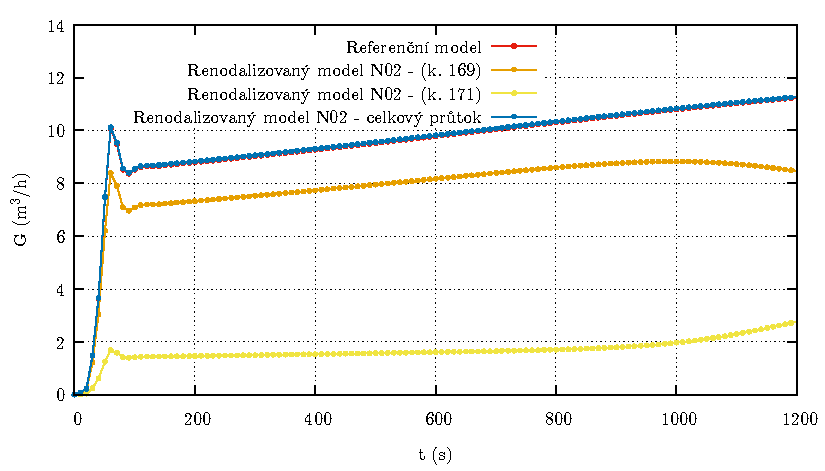
\includegraphics[width=.8\textwidth]{./05_TH_model_VR_1/grafy/nod_02_mass_flow_rate_vertical}
	\caption{Průtok skrze AZ reaktoru VR-1 - referenční a renodalizovaný model NOD02.}
	\label{fig:nod_02_mass_flow_rate_vertical}
\end{figure}
\begin{figure}[H]
	\centering
	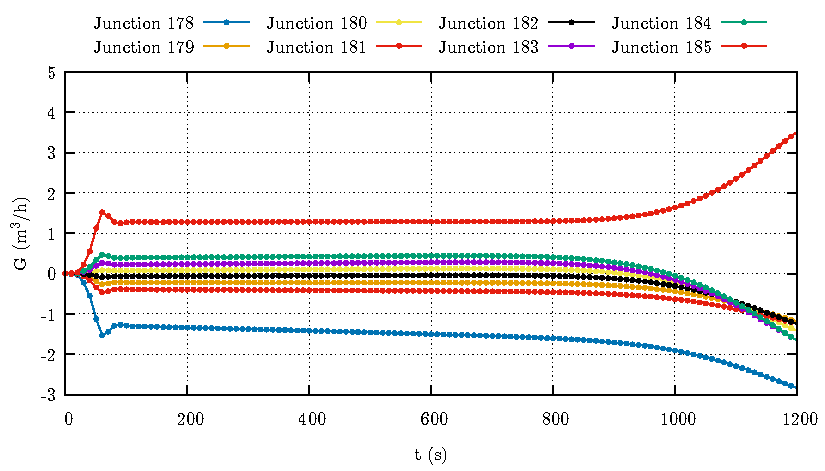
\includegraphics[width=0.8\textwidth]{./05_TH_model_VR_1/grafy/nod_02_mass_flow_rate_horizontal.pdf}
	\caption{Průtok spojovacími jednotkami (SJ) ve vertikálním obtoku - model NOD02.}
	\label{fig:nod_02_mass_flow_rate_horizontal}
\end{figure}
%\begin{figure}[H]
%	\centering
%	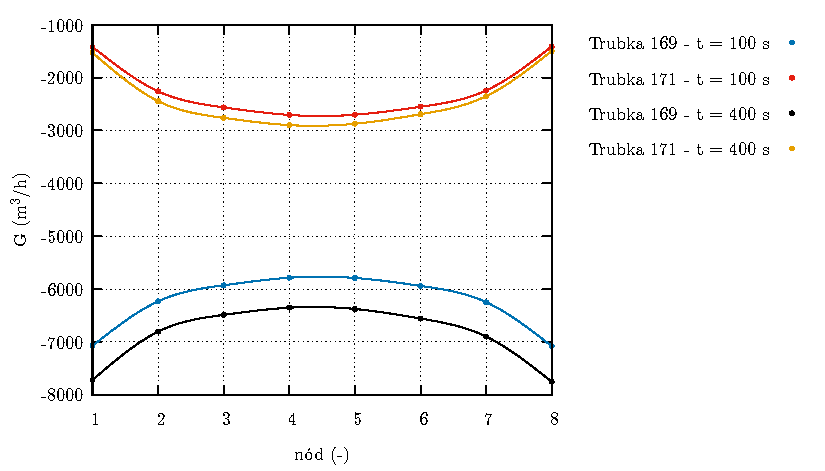
\includegraphics[width=0.8\textwidth]{./05_TH_model_VR_1/grafy/nod_02_vertikal_obtok.pdf}
%	\caption{Průtok v jednotlivých nódech trubek 169 a 171.}
%	\label{fig:nod_02_vertikal_obtok}
%\end{figure}
\begin{figure}[H]
	\centering
	\includegraphics[width=0.8\textwidth]{./05_TH_model_VR_1/grafy/t_nod_02.pdf}
	\caption{Teplotní vývoj v trubce 40 - model NOD02.}
	\label{fig:nod_02_temp_pipe_40}
\end{figure}
\section{Model NOD03}
\label{sec:nod_03}
Model reaktoru NOD03 rozvíjí možnost vzniku recirkulace ve volném objemu vody nad aktivní zónou reaktoru. Horizontálně orientované trubky jsou nahrazeny vertikálními, které jsou propojeny pomocí spojovacích jednotek. Díky tomu může voda proudit v každé trubce po celé výšce vodního sloupce nad aktivní zónou reaktoru. Model je uveden v příloze na obr. \ref{fig:nod_03_prilohy}. Objem horizontálního obtoku (součet všech kontrolních objemů) je zachován. Konstrukce a směry proudění jsou ilustrovány na obr. \ref{fig:nod_03}. Spoje jsou rozděleny do skupin S1 až S8 pro lepší orientaci.

Je otázkou, zda jsou následující výsledky reprezentativní a mají fyzikální význam. Hlavním problémem je stabilita výpočtu, která není zaručena a při takto komplexním proudění může dojít k nesprávným řešením viz následující sekce.
  \begin{figure}[H]
 	\centering
 	\includegraphics[width=\textwidth,  trim={7.5cm 243cm 155cm 5cm}, clip]{./07_prilohy/recirkulace/nod_03_recirculation.pdf}
 	\caption{Nodalizace horizontálního obtoku - model NOD03}
 	\label{fig:nod_03}
 \end{figure}
 \subsection{Výsledky}
V souladu s předchozími případy je na obrázku \ref{fig:nod_03_mass_flow_rate_vertical} prezentováno srovnání průtoku skrze AZ s referenčním modelem. V porovnání s modelem NOD01 lze pozorovat podobné chování, přičemž kolem 200 s dochází k ustálení toku na kvazistacionární hodnotu (viz obrázek \ref{fig:nod_01_mass_flow_rate_vertical}). Průtok v jednotlivých skupinách SJ je problematický a chaotický, přičemž k ustálení průtoku nedochází viz obr. \ref{fig:nod_03_mass_flow_rate_horizontal_s3} a \ref{fig:nod_03_mass_flow_rate_horizontal_s4}. Grafy pro všechny skupiny jsou uvedeny v příloze viz obr. \ref{fig:g_time_nod_03_0_prilohy} až \ref{fig:g_time_nod_03_5_prilohy}.
\begin{figure}[H]
	\centering
	\begin{subfigure}{0.5\textwidth}
		\centering
		\includegraphics[width=\textwidth, trim={0cm 0cm 0cm 0cm}, clip]{./05_TH_model_VR_1/grafy/G_time_nod_03_2.pdf}
		\caption{S3}
		\label{fig:nod_03_mass_flow_rate_horizontal_s3}
	\end{subfigure}%
	\hfill
	\begin{subfigure}{0.5\textwidth}
		\centering
		\includegraphics[width=\textwidth, trim={0cm 0cm 0cm 0cm}, clip]{./05_TH_model_VR_1/grafy/G_time_nod_03_3.pdf}
		\caption{S4}
		\label{fig:nod_03_mass_flow_rate_horizontal_s4}
	\end{subfigure}%
	\caption{Průtok skrze jednotlivé SJ (S3 a S4) - model NOD03.}
\end{figure}
V obrázku \ref{fig:nod_03_temp_pipe_40} jsou vykresleny teploty chladiva v jednotlivých nódech trubky 40. Na rozdíl od celkového průtoku je časový vývoj teplot analogický spíše referenčnímu modelu. 
  \begin{figure}[H]
 	\centering
 	\includegraphics[width=0.8\textwidth]{./05_TH_model_VR_1/grafy/nod_03_mass_flow_rate_vertical.pdf}
 	\caption{Průtok skrze AZ reaktoru VR-1 - referenční a renodalizovaný model NOD03. }
 	\label{fig:nod_03_mass_flow_rate_vertical}
 \end{figure}
% \begin{figure}[H]
% 	\centering
% 	\includegraphics[width=0.8\textwidth]{./05_TH_model_VR_1/grafy/G_time_.pdf}
% 	\caption{Průtok skrze trubky 170 - 174 (viz obr. \ref{fig:nod_01}) - renodalizovaný model NOD01.}
% 	\label{fig:nod_03_mass_flow_rate_horizontal}
% \end{figure}
 \begin{figure}[H]
 	\centering
 	\includegraphics[width=0.8\textwidth]{./05_TH_model_VR_1/grafy/t_nod_03.pdf}
 	\caption{Teplotní vývoj v trubce 40 - model NOD03.}
 	\label{fig:nod_03_temp_pipe_40}
 \end{figure}
% \begin{figure}[H]
% 	\centering
% 	\includegraphics[width=0.8\textwidth]{./05_TH_model_VR_1/grafy/nod_01_900.pdf}
% 	\caption{Distribuce teplot v trubce 40 v čase 900 s.}
% 	\label{fig:nod_01_temp_distribution}
% \end{figure}
% 
 \section{Model NOD04}
 \label{sec:nod_04}
Poslední a nejkomplexnější varianta termohydraulického modelu VR-1 je modifikace modelu NOD03, která částečně vychází z práce \cite{CAPABILITY2017RELAP}. Výsledky získané pro model NOD03 naznačují, že nedochází k ustálení průtoku chladiva skrze jednotlivé skupiny spojovacích jednotek S1 až S6 (více na Obr. \ref{fig:g_time_nod_03_0_prilohy} až \ref{fig:g_time_nod_03_5_prilohy} v příloze). Důvodem fyzikálně neodpovídajících výsledků je nedostatečně propojená vodní hladina s trubkami horizontálního obtoku. Například kapalina v nódu 5 trubky 231 by musela projít minimálně dalšími 11 komponentami než by dorazila do TDV 50 viz obr. \ref{fig:nod_03}. Proto byla do modelu přidána vícenásobná spojovací jednotka (BRANCH) 233 a kontrolní objem 232, které propojují vodní hladinu se všemi skupinami S1 až S6. 
  \begin{figure}[H]
	\centering
\includegraphics[width=0.8\textwidth, trim={7.5cm 243cm 155cm 0cm}, clip]{./07_prilohy/recirkulace/nod_04_recirculation.pdf}
	\caption{Nodalizace horizontálního obtoku - model NOD04}
	\label{fig:nod_04}
\end{figure}
 \subsection{Výsledky}
Na obrázku \ref{fig:nod_04_mass_flow_rate_vertical} je zobrazen celkový průtok chladiva skrze AZ pro referenční model a modely NOD01, NOD03 a NOD04. V případě modelu NOD04 je celkový průtok téměř shodný s modelem NOD03. Dochází však k drastické změně směru proudění ve všech skupinách spojovacích jednotek (SJ), jak je vidět na obrázcích \ref{fig:nod_03} a \ref{fig:nod_04}. Díky odlišné konstrukci vodní hladiny dochází k relativnímu ustálení průtoku v čase okolo 800 s, jak je patrné z obr. \ref{fig:nod_04_mass_flow_rate_horizontal_s3} a \ref{fig:nod_04_mass_flow_rate_horizontal_s4}. Průtok skrze ostatní skupiny je uveden v příloze na obr. \ref{fig:g_time_nod_04_0_prilohy} až \ref{fig:g_time_nod_04_5_prilohy}.
\begin{figure}[H]
	\centering
	\includegraphics[width=0.8\textwidth]{./05_TH_model_VR_1/grafy/nod_04_mass_flow_rate_vertical.pdf}
	\caption{Průtok skrze AZ reaktoru VR-1 - Referenční model a renodalizovaný model NOD01, NOD03 a NOD04.}
	\label{fig:nod_04_mass_flow_rate_vertical}
\end{figure}
\begin{figure}[H]
	\centering
	\begin{subfigure}{0.5\textwidth}
		\centering
		\includegraphics[width=\textwidth, trim={0cm 0cm 0cm 0cm}, clip]{./05_TH_model_VR_1/grafy/G_time_nod_04_2.pdf}
		\caption{S3}
		\label{fig:nod_04_mass_flow_rate_horizontal_s3}
	\end{subfigure}%
	\hfill
	\begin{subfigure}{0.5\textwidth}
		\centering
		\includegraphics[width=\textwidth, trim={0cm 0cm 0cm 0cm}, clip]{./05_TH_model_VR_1/grafy/G_time_nod_04_3.pdf}
		\caption{S4}
		\label{fig:nod_04_mass_flow_rate_horizontal_s4}
	\end{subfigure}%
	\caption{Průtok skrze jednotlivé SJ (S3 a S4) - model NOD04.}
\end{figure}
 \begin{figure}[H]
 	\centering
 	\includegraphics[width=0.8\textwidth]{./05_TH_model_VR_1/grafy/tempf_nod_04_1.pdf}
 	\caption{Teplotní vývoj v trubce 40 - model NOD04.}
 \end{figure}
 
 
 
 
 
\chapter{Hodnocení termohydraulických modelů}
V této studii bylo zkoumáno 5 různých nodalizací termohydraulického modelu reaktoru VR-1 v programu RELAP5. V této kapitole jsou všechny modely srovnány mezi sebou, porovnány s daty z reaktoru Triga Mark II a okomentovány v souvislosti s bezpečnostními analýzami.

Z analýzy vyplynulo, že referenční model (NOD00) a renodalizovaný model NOD02 mají odlišné chování v porovnání s modely NOD01 a NOD04. Tyto modely neumožňují vzniku recirkulace ve volném objemu na AZ v horizontálním obtoku a dochází k nadhodnocení celkového průtoku (komentář k této problematice je uveden v kapitole \ref{chap:th_model_vr_1}). Toto nadhodnocení vede díky lepšímu odvodu tepla k celkově nižší výstupní teplotě chladiva. Pro kontext  jsou na obr. \ref{fig:cfd_triga_temperatures_velocities} uvedeny grafy využité k validaci termohydraulického CFD modelu reaktoru TRIGA Mark I \cite{TRIGA_CFD}. V \cite{TRIGA_CFD} je předpokládán přechodový jev (exkurze výkonu na konstantní hodnotu) za vzniku ustáleného přirozeného proudění, detailní průběh výkonu ale není doložen. Chování průměrných teplot a rychlostí v AZ reaktoru TRIGA lze vztáhnout k výsledkům uvedeným na obr. \ref{fig:G_stationary_100} a \ref{fig:T_out_stationary_100}.


\begin{figure}[H]
	\centering
	\begin{minipage}{.5\textwidth}
		\centering
		\includegraphics[width=\textwidth, trim={1cm 7cm 1cm 7cm}, clip]{./06_hodnoceni_TH_modelu/obrazky/cfd_triga_temperatures.pdf}
%		\caption{teploty}
%		\label{fig:cfd_triga_temperatures}
	\end{minipage}%
	\begin{minipage}{.5\textwidth}
		\centering
		\includegraphics[width=\linewidth, trim={1cm 7cm 1cm 7cm}, clip]{./06_hodnoceni_TH_modelu/obrazky/cfd_triga_mass_flow_rate.pdf}
%		\caption{Průměrné rychlosti}
%		\label{fig:cfd_triga_mass_flow_rate}
	\end{minipage}
	\caption{Průměrné teploty a rychlosti v jednotlivých částech AZ reaktoru TRIGA Mark II (CFD výpočet) \cite{TRIGA_CFD}.}
	\label{fig:cfd_triga_temperatures_velocities}
\end{figure}
\begin{figure}[H]
	\centering
	\begin{minipage}{.5\textwidth}
		\centering
		\includegraphics[width=\textwidth]{./06_hodnoceni_TH_modelu/grafy/G_stationary_100_trans.pdf}
%		\caption{Přechodový stav.}
%		\label{fig:G_stationary_100_trans}
	\end{minipage}%
	\begin{minipage}{.5\textwidth}
		\centering
		\includegraphics[width=\linewidth]{./06_hodnoceni_TH_modelu/grafy/G_stationary_100.pdf}
%		\caption{Kvazistacionární stav.}
		
	\end{minipage}
	\caption{Průtok skrz AZ reaktoru VR-1 pro jednotlivé modely (RELAP5).}
	\label{fig:G_stationary_100}
\end{figure}

Z porovnání obr. \ref{fig:G_stationary_100} lze soudit, že průtok v referenčním modelu a modelu NOD02 neodpovídá chování CFD výpočtu uvedenému na obr. \ref{fig:cfd_triga_temperatures_velocities}. Vzhledem k vyššímu průtoku a tedy lepšímu odvodu tepla se modely NOD00 a NOD02 jeví jako méně konzervativní. Proto by pro výpočet přechodových jevů v rámci bezpečnostních analýz bylo vhodnější využít modely NOD01 a NOD04, které mají nižší a konstantní průtok a tedy se zdají být konzervativnější a stabilnější. Z důvodu nestability popsané v sekci \ref{sec:nod_03} (špatné konstrukce vodní hladiny) není vhodné používat model NOD03 pro další analýzy.

Teplota na výstupu z AZ je nejvyšší v případě modelu NOD01, tedy model se pro analýzu přechodových jevů zdá být v rámci zkoumaných modelů nejvíce konzervativní.
\begin{figure}[H]
	\centering
	\begin{minipage}{.5\textwidth}
		\centering
		\includegraphics[width=\textwidth]{./06_hodnoceni_TH_modelu/grafy/T_out_stationary_100_trans.pdf}
		%		\caption{Přechodový stav.}
		%		\label{fig:T_out_stationary_100_trans}
	\end{minipage}%
	\begin{minipage}{.5\textwidth}
		\centering
		\includegraphics[width=\linewidth]{./06_hodnoceni_TH_modelu/grafy/T_out_stationary_100.pdf}
		%		\caption{Kvazistacionární stav.}
		
	\end{minipage}
	\caption{Teploty chladiva na výstupu z AZ reaktoru VR-1 pro jednotlivé modely (RELAP5).}
	\label{fig:T_out_stationary_100}
\end{figure}




\begin{figure}[H]
	\centering
	\begin{minipage}{.5\textwidth}
		\centering
		\includegraphics[width=\textwidth]{./06_hodnoceni_TH_modelu/grafy/T_in_stationary_102_long.pdf}
		\caption{Vstupní teplota chladiva pro jednotlivé modely (RELAP5)}
		\label{fig:T_in_stationary_102_long}
	\end{minipage}%
	\begin{minipage}{.5\textwidth}
		\centering
		\includegraphics[width=\linewidth]{./06_hodnoceni_TH_modelu/grafy/T_out_stationary_100_long.pdf}
		\caption{Výstupní teplota chladiva pro jednotlivé modely (RELAP5).}
		\label{fig:T_out_stationary_100_long}
	\end{minipage}
	
\end{figure}

Dále platí, že doba, než dojde k úplné recirkulaci a tedy k nárůstu teploty na vstupu do AZ, je nejnižší u modelů NOD03 a NOD04. Tato skutečnost vyplývá z obr. \ref{fig:T_in_stationary_102_long}. Po dobu kolem 4000 s je vstupní teplota chladiva konstantní. Následně dochází ke schodovitému nárůstu, u kterého lze spekulovat o fyzikálním odůvodnění. Čas 4000 s ovšem odpovídá rychlosti proudění a konstrukci reaktoru, tedy jako původ tohoto nárůstu lze považovat vstup ohřáté kapaliny do AZ. Model NOD02 není uveden, neboť má identické chování jako referenční model.

\begin{figure}[H]
 	\centering
 	\begin{minipage}{.5\textwidth}
 		\centering
 		\includegraphics[width=\textwidth]{./06_hodnoceni_TH_modelu/grafy/G_stationary_100_long.pdf}
 		
 	\end{minipage}%
 	
 	\caption{Průtok skrz AZ reaktoru VR-1 pro jednotlivé modely (RELAP5).}
 	\label{fig:G_stationary_100_long}
\end{figure}

Ohřev celkového objemu v reaktorové nádobě vede u všech modelů k poklesu teplotního gradientu a tedy i ke klesajícímu průtoku viz obr. \ref{fig:G_stationary_100_long}. 



Pro úplnost jsou v tab. \ref{tab:teploty_hs} uvedeny průměrné a maximální teploty HS pro jednotlivé modely. Opět se jako nejkonzervativnější jeví model NOD01, kdy je průměrná a maximální teplota HS nejvyšší. V rámci výpočtů lze ovšem rozdíly mezi jednotlivými modely považovat za zanedbatelné.
\begin{table}[H]
	\centering
	\caption{Maximální a průměerné teploty HS pro jednotlivé modely.}
	\label{tab:teploty_hs}
	\begin{tabular}{ccc}
		\hline
		Model	&	$ T_{\text{av}} $ (K)	& $ T_{\text{max}} $ (K)	\\
		\hline
		\hline
		NOD00	&	308,7	&	 313,6	 \\
		NOD01	&	309,5	&	 314,9	 \\
		NOD02	&	308,7	&	 313,6	 \\
		NOD03	& 	309,2	&	 314,4	 \\
		NOD04	&	309,2	&	 314,3	 \\
		\hline
	\end{tabular}
\end{table} 





Celkově z uvedených výsledků vyplývá, že jako vhodné pro analýzu přechodových se jeví renodalizované termohydraulické modely NOD01 a NOD04. V obou případech je charakteristika přirozeného proudění stabilní a chováním odpovídá \cite{TRIGA_CFD}. Pro bezpečnostní analýzy se může zdát vhodnější model NOD01, který je v porovnání s ostatními modely nejkonzervativnější.




%\begin{figure}[H]
%	\centering
%	\begin{minipage}{.5\textwidth}
%		\centering
%		\includegraphics[width=\textwidth]{./06_hodnoceni_TH_modelu/obrazky/cfd_triga_temperatures_az_odd.png}
%		\caption{Lichá sada termočlánků.}
%		\label{fig:cfd_triga_temperatures_az_odd}
%	\end{minipage}%
%	\begin{minipage}{.5\textwidth}
%		\centering
%		\includegraphics[width=\linewidth]{./06_hodnoceni_TH_modelu/obrazky/cfd_triga_temperatures_az_even.png}
%		\caption{Sudá sada termočlánků.}
%		\label{fig:cfd_triga_temperatures_az_even}
%	\end{minipage}
%	\caption{Teploty v jednotlivých částech AZ reaktoru TRIGA Mark II - (Experiment a CFD výpočet) \cite{TRIGA_CFD}.}
%\end{figure}





%\input{vnitrek_kapitola1.tex} % text vkládán ze souboru. Pokud je v souboru uveden i příkaz \chapter{...}, tak ho o 4 řádky výše vymažte.


\chapter*{Závěr} % SEM NESAHEJTE!
\addcontentsline{toc}{chapter}{Závěr} % SEM NESAHEJTE!
%\input{./06_zaver/zaver.tex}


%%%%%%%%%%%% SEZNAM POUŽITÝCH ZDROJŮ (LITERATURA) %%%%%%%%%%%%
%\clearpage  % SEM NESAHEJTE!
%\addcontentsline{toc}{chapter}{Literatura} % SEM NESAHEJTE!



\bibliographystyle{plain}
\bibliography{ref} 
%\begin{thebibliography}{99}   
%	% formát: ČSN ISO 690. Můžete si to vygenerovat na http://www.citacepro.com (přihlaste se přes odkaz "ČVUT"), umí to vygenerovat TeX
%	% řazení: abecedně podle autora (resp. prvního slova, není-li znám autor)
%	\bibitem{odkaz} Autor. \ti{Název knihy}. Město. Nakladatelství. Rok.  
%\end{thebibliography}


%%%%%%%%%%%% PŘÍLOHY PRÁCE %%%%%%%%%%%%
\newpage % SEM NESAHEJTE!
\addcontentsline{toc}{chapter}{Přílohy} % SEM NESAHEJTE!
\appendix % SEM NESAHEJTE!


%%%%%%%%%%%% Příloha A (tj. 1. kapitola v rámci příloh) %%%%%%%%%%%%
\chapter{Přehled modelů}
\begin{table}[H]
	\centering
	
	\caption{Přehled použitých modelů PČ IRT-4M (Modely označené hvězdičkou byly vytvořeny i pro 6-trubkovou a 4-trubkovou konfiguraci).}
	\begin{tabular}{ccc}
		\hline
		Hydraulické modely & Název modelu & Popsán v sekci: \\
		\hline \hline
							& Komplexní model PČ bez vytěsnitele & \ref{sec:hydraulicky_model_irt}  \\
							& Komplexní model PČ s vytěsnitelem & \ref{sec:hydraulicky_model_irt} \\
							& Zjednodušený model PČ bez vytěsnitele & \ref{sec:zjednoduseny_hydraulicky_model_irt}\\
							& Zjednodušený model PČ s vytěsnitelem & \ref{sec:zjednoduseny_hydraulicky_model_irt} \\
		\hline
		Termohydraulické modely &  Název modelu & Popsán v sekci: \\
			\hline \hline
							& Komplexní model PČ bez vytěsnitele & \ref{sec:termohydraulicky_model_IRT}  \\
							& Zjednodušený model PČ bez vytěsnitele & \ref{sec:termohydraulicky_model_IRT}\\
							& Jednotkový model PČ & \ref{sec:sjednoceni_topnych_komponent} \\
			\hline				
	\end{tabular}
\end{table}

\begin{table}[H]
	\centering
	
	\caption{Přehled nodalizací modelu školního reaktoru VR-1.}
	\begin{tabular}{ccc}
		\hline
		
		Termohydraulické modely &  Název modelu & Popsán v sekci: \\
		\hline \hline
		& Referenční model / Model NOD00  &  \ref{sec:referencni_model}\\
		& Model N0D01 & \ref{sec:nod_01}\\
		& Model N0D02 & \ref{sec:nod_02}\\
		& Model N0D03 & \ref{sec:nod_03}\\
		& Model NOD04 & \ref{sec:nod_04}\\
		\hline				
	\end{tabular}
\end{table}
\chapter{Tabulky}
%

\begin{table}[H]
	\centering
	\caption{Geometrie 8-trubkového palivového článku IRT-4M \cite{sedlbauer2019}}
	\label{tab:prilohy_irt_geometrie}
	\begin{tabular}{ccccccccc}
		\hline
		Číslo trubky & 1 & 2 & 3 & 4 & 5 & 6 & 7 & 8 \\
		\hline \hline
		Vnější rozměr trubky (mm) & 69,6  & 62,7  & 55,8  & 48,9  & 42,0  & 35,1  & 28,2  & $\oslash$ 21,3 \\
		Vnitřní rozměr trubky (mm)  &   66,4 & 59,5 & 52,6 & 45,7 & 38,8 & 31,9 & 25  & $\oslash$ 18,1 \\
		\hline
		Vnější rozměr palivové vrstvy &  68,7 & 61,8 & 54,9 & 48,0 & 41,1 & 34,2 & 27,3 & $\oslash$ 20,4 \\
		Vnitřní rozměr palivové vrstvy &  67,3 & 60,4 & 53,5 & 46,6 & 39,7 & 32,8 & 25,9 & $\oslash$ 19,0 \\
		\hline
		Vnější poloměr zakřivení & 9,3 & 8,5 & 7,7 & 6,9 & 6,1 & 5,3 & 4,5 & - \\
		Vnitřní poloměr zakřivení & 7,7 & 6,9 & 6,1 & 5,3 & 4,5 & 3,7 & 2,9 & - \\
		\hline
		\hline
		
		Vnější průměr vytěsnitele (mm) & 14 & & & & & & & \\
		Vnitřní průměr vytěsnitele (mm) & 12 & & & & & & & \\
		Průměr vstupního otvoru vytěsnitele (mm) & 3 & & & & & & & \\
		\hline 
		 
	\end{tabular}
\end{table}

\begin{table}[H]
	\centering
	\caption{Průběh výkonu jednoho PČ.}
	\label{tab:vykon_model}
	\begin{tabular}{cc}
		\hline
		t (s) & P (W) \\
		\hline
		
		0  & 0  \\
		10 & 100 \\
		15 & 1000 \\
		20 & $ 10^4 $ \\
		30 & $ 10^4$ \\
		\multicolumn{2}{c}{\textellipsis} \\
		1200 & $ 10^4 $ \\
		\hline
	\end{tabular}
	
	
\end{table}


%\begin{table}[H]
%	\centering
%	\caption{Geometrie horizontálního obtoku - referenční model}
%	\label{tab:geometrie_ref_hor}
%	\begin{tabular}{ccc}
%		\hline
%		& Trubka 40 & Trubka 42 \\
%		\hline
%		Průměr (m) & 2,3000 & 1,2365 \\ 
%		Průtočná plocha (m$^2$) & 4,1548 & 1,2008 \\
%		Délka (m) & 1,2365 & 1,2500 \\
%		\hline
%	\end{tabular}
%\end{table}
%\begin{table}[H]
%	\centering
%	\caption{Geometrie vertikálního obtoku - referenční model}
%	\label{tab:geometrie_ref_ver}
%	\begin{tabular}{cc}
%		\hline 
%		& Trubka 44 \\
%		\hline
%		Průměr (m): & 2,3 \\
%		Průtočná plocha (m$^2$) & 4,1548 \\
%		Délka (m) & 3,955 \\
%		\hline
%	\end{tabular}
%\end{table}
\chapter{Obrázky}
\begin{figure}
	\centering
	\includegraphics[width=\textwidth, trim={1cm 5cm 1cm 4cm}, clip]{./07_prilohy/obrazky/vr_1_geometrie.pdf}
	\caption{Konstrukce reaktoru VR-1 \cite{BILY201997}.}
	\label{fig:vr_1_geometrie}
\end{figure}
\begin{figure}
	\centering
	\includegraphics[width=\textwidth, trim={0cm 0cm 0cm 0cm}, clip]{./07_prilohy/obrazky/triga_geometrie.pdf}
	\caption{Konstrukce reaktoru TRIGA Mark I \cite{TRIGA_CFD}.}
	\label{fig:triga_geometrie}
\end{figure}

\begin{figure}
	\centering
	\includegraphics[width=\textwidth, trim={0cm 218cm 148cm 5cm}, clip]{./07_prilohy/prehled_modelu/nod00.pdf}
	\caption{Termohydraulický model reaktoru VR-1 - Referenční model (NOD00).}
	\label{fig:nod_00_prilohy}
\end{figure}
\begin{figure}
	\centering
	\includegraphics[width=\textwidth, trim={0cm 218cm 148cm 5cm}, clip]{./07_prilohy/prehled_modelu/nod01.pdf}
	\caption{Termohydraulický model reaktoru VR-1 - model NOD01.}
	\label{fig:nod_01_prilohy}
\end{figure}
\begin{figure}
	\centering
	\includegraphics[width=\textwidth, trim={0cm 218cm 148cm 5cm}, clip]{./07_prilohy/prehled_modelu/nod02.pdf}
	\caption{Termohydraulický model reaktoru VR-1 - model NOD02.}
	\label{fig:nod_02_prilohy}
\end{figure}
\begin{figure}
	\centering
	\includegraphics[width=\textwidth, trim={0cm 218cm 148cm 5cm}, clip]{./07_prilohy/prehled_modelu/nod03.pdf}
	\caption{Termohydraulický model reaktoru VR-1 - model NOD03.}
	\label{fig:nod_03_prilohy}
\end{figure}
\begin{figure}
	\centering
	\includegraphics[width=\textwidth, trim={0cm 214cm 148cm 0cm}, clip]{./07_prilohy/prehled_modelu/nod04.pdf}
	\caption{Termohydraulický model reaktoru VR-1 - Model NOD04}
\end{figure}
\begin{figure}
	\centering
	\begin{subfigure}{0.5\textwidth}
		\centering
		\includegraphics[width=\textwidth, trim={0cm 0cm 0cm 0cm}, clip]{./05_TH_model_VR_1/grafy/temp_rozl/t_rozl_100.pdf}
		\caption{t = 100 s}
		\label{fig:temp_dist_srovnani_prilohy_100s}
	\end{subfigure}%
	\hfill
	\begin{subfigure}{0.5\textwidth}
		\centering
		\includegraphics[width=\textwidth, trim={0cm 0cm 0cm 0cm}, clip]{./05_TH_model_VR_1/grafy/temp_rozl/t_rozl_200.pdf}
		\caption{t = 200}
		\label{fig:temp_dist_srovnani_prilohy_200s}
	\end{subfigure}
	\caption{Rozložení teplot v trubce 40}
\end{figure}
\begin{figure}
	\centering
	\begin{subfigure}{0.5\textwidth}
		\centering
		\includegraphics[width=\textwidth, trim={0cm 0cm 0cm 0cm}, clip]{./05_TH_model_VR_1/grafy/temp_rozl/t_rozl_300.pdf}
		\caption{t = 300 s}
		\label{fig:temp_dist_srovnani_prilohy_300s}
	\end{subfigure}%
	\hfill
	\begin{subfigure}{0.5\textwidth}
		\centering
		\includegraphics[width=\textwidth, trim={0cm 0cm 0cm 0cm}, clip]{./05_TH_model_VR_1/grafy/temp_rozl/t_rozl_400.pdf}
				\caption{t = 400 s}
		\label{fig:temp_dist_srovnani_prilohy_400s}
	\end{subfigure}
	\caption{Rozložení teplot v trubce 40.}
\end{figure}
\begin{figure}
	\centering
	\begin{subfigure}{0.5\textwidth}
		\centering
		\includegraphics[width=\textwidth, trim={0cm 0cm 0cm 0cm}, clip]{./05_TH_model_VR_1/grafy/temp_rozl/t_rozl_500.pdf}
				\caption{t = 500 s}
		\label{fig:temp_dist_srovnani_prilohy_500s}
	\end{subfigure}%
	\hfill
	\begin{subfigure}{0.5\textwidth}
		\centering
		\includegraphics[width=\textwidth, trim={0cm 0cm 0cm 0cm}, clip]{./05_TH_model_VR_1/grafy/temp_rozl/t_rozl_600.pdf}
				\caption{t = 600 s}
		\label{fig:temp_dist_srovnani_prilohy_600s}
	\end{subfigure}
	\caption{Rozložení teplot v trubce 40.}
\end{figure}


\begin{figure}
	\centering
	\begin{subfigure}{0.5\textwidth}
		\centering
		\includegraphics[width=\textwidth, trim={0cm 0cm 0cm 0cm}, clip]{./05_TH_model_VR_1/grafy/G_time_nod_03_0.pdf}
				\caption{S1}
		\label{fig:g_time_nod_03_0_prilohy}
	\end{subfigure}%
	\hfill
	\begin{subfigure}{0.5\textwidth}
	\centering
	\includegraphics[width=\textwidth, trim={0cm 0cm 0cm 0cm}, clip]{./05_TH_model_VR_1/grafy/G_time_nod_03_1.pdf}
			\caption{S2}
	\label{fig:g_time_nod_03_1_prilohy}
\end{subfigure}%
	\caption{Průtok skupinou S1 a S2 - model NOD03.}
\end{figure}
\begin{figure}
	\centering
	\begin{subfigure}{0.5\textwidth}
		\centering
		\includegraphics[width=\textwidth, trim={0cm 0cm 0cm 0cm}, clip]{./05_TH_model_VR_1/grafy/G_time_nod_03_2.pdf}
				\caption{S3}
		\label{fig:g_time_nod_03_2_prilohy}
	\end{subfigure}%
	\hfill
	\begin{subfigure}{0.5\textwidth}
		\centering
		\includegraphics[width=\textwidth, trim={0cm 0cm 0cm 0cm}, clip]{./05_TH_model_VR_1/grafy/G_time_nod_03_3.pdf}
				\caption{S4}
		\label{fig:g_time_nod_03_3_prilohy}
	\end{subfigure}%
	\caption{Průtok skupinou S3 a S4 - model NOD03.}
\end{figure}
\begin{figure}
	\centering
	\begin{subfigure}{0.5\textwidth}
		\centering
		\includegraphics[width=\textwidth, trim={0cm 0cm 0cm 0cm}, clip]{./05_TH_model_VR_1/grafy/G_time_nod_03_4.pdf}
		\caption{S5}
		\label{fig:g_time_nod_03_4_prilohy}
	\end{subfigure}%
	\hfill
	\begin{subfigure}{0.5\textwidth}
		\centering
		\includegraphics[width=\textwidth, trim={0cm 0cm 0cm 0cm}, clip]{./05_TH_model_VR_1/grafy/G_time_nod_03_5.pdf}
				\caption{S6}
		\label{fig:g_time_nod_03_5_prilohy}
	\end{subfigure}%
	\caption{Průtok skupinou S5 a S6 - model NOD03.}
\end{figure}

\begin{figure}
	\centering
	\begin{subfigure}{0.5\textwidth}
		\centering
		\includegraphics[width=\textwidth, trim={0cm 0cm 0cm 0cm}, clip]{./05_TH_model_VR_1/grafy/G_time_nod_04_0.pdf}
		\caption{S1}
		\label{fig:g_time_nod_04_0_prilohy}
	\end{subfigure}%
	\hfill
	\begin{subfigure}{0.5\textwidth}
		\centering
		\includegraphics[width=\textwidth, trim={0cm 0cm 0cm 0cm}, clip]{./05_TH_model_VR_1/grafy/G_time_nod_04_1.pdf}
		\caption{S2}
		\label{fig:g_time_nod_04_1_prilohy}
	\end{subfigure}%
	\caption{Průtok skupinou S1 a S2 - model NOD04.}
\end{figure}
\begin{figure}
	\centering
	\begin{subfigure}{0.5\textwidth}
		\centering
		\includegraphics[width=\textwidth, trim={0cm 0cm 0cm 0cm}, clip]{./05_TH_model_VR_1/grafy/G_time_nod_04_2.pdf}
		\caption{S3}
		\label{fig:g_time_nod_04_2_prilohy}
	\end{subfigure}%
	\hfill
	\begin{subfigure}{0.5\textwidth}
		\centering
		\includegraphics[width=\textwidth, trim={0cm 0cm 0cm 0cm}, clip]{./05_TH_model_VR_1/grafy/G_time_nod_04_3.pdf}
		\caption{S4}
		\label{fig:g_time_nod_04_3_prilohy}
	\end{subfigure}%
	\caption{Průtok skupinou S3 a S4 - model NOD04.}
\end{figure}
\begin{figure}
	\centering
	\begin{subfigure}{0.5\textwidth}
		\centering
		\includegraphics[width=\textwidth, trim={0cm 0cm 0cm 0cm}, clip]{./05_TH_model_VR_1/grafy/G_time_nod_04_4.pdf}
		\caption{S5}
		\label{fig:g_time_nod_04_4_prilohy}
	\end{subfigure}%
	\hfill
	\begin{subfigure}{0.5\textwidth}
		\centering
		\includegraphics[width=\textwidth, trim={0cm 0cm 0cm 0cm}, clip]{./05_TH_model_VR_1/grafy/G_time_nod_04_5.pdf}
		\caption{S6}
		\label{fig:g_time_nod_04_5_prilohy}
	\end{subfigure}%
	\caption{Průtok skupinou S5 a S6 - model NOD04.}
\end{figure}
%
%\input{priloha_A.tex} % text vkládán ze souboru, kde je i příkaz \chapter{...}


\end{document} % SEM NESAHEJTE! Konec.
